%%%%%%%%%%%%%%%%%%%%%%%%%%%%%%%%%%%%%%%%%%%%%%%%%%%%%%%%%%%%%%%%%%%%%%
%%  disstemplate.tex, to be compiled with latex.                    %%
%%  08 April 2002 Version 5                                         %%
%%%%%%%%%%%%%%%%%%%%%%%%%%%%%%%%%%%%%%%%%%%%%%%%%%%%%%%%%%%%%%%%%%%%%%
%%                                                                  %%
%%  Writing a Doctoral Dissertation with LaTeX at                   %%
%%  the University of Texas at Austin                               %%
%%                                                                  %%
%%  (Modify this ``template'' for your own dissertation.)           %%
%%                                                                  %%
%%%%%%%%%%%%%%%%%%%%%%%%%%%%%%%%%%%%%%%%%%%%%%%%%%%%%%%%%%%%%%%%%%%%%%


\documentclass[12pt]{report}    % The documentclass must be ``report''.

\usepackage{utdiss2}            % Dissertation package style file.


%%%%%%%%%%%%%%%%%%%%%%%%%%%%%%%%%%%%%%%%%%%%%%%%%%%%%%%%%%%%%%%%%%%%%%
% Optional packages used for this sample dissertation. If you don't  %
% need a capability in your dissertation, feel free to comment out   %
% the package usage command.                                         %
%%%%%%%%%%%%%%%%%%%%%%%%%%%%%%%%%%%%%%%%%%%%%%%%%%%%%%%%%%%%%%%%%%%%%%

% Some packages to write mathematics.
\usepackage{amsmath,amsthm,amsfonts,amscd} 
\usepackage{eucal}      % Euler fonts
\usepackage{verbatim}   % Allows quoting source with commands.
\usepackage{makeidx}    % Package to make an index.
\usepackage{epsfig}     % Allows inclusion of eps files.
%\usepackage{citesort}  % citesort is ancient and deprecated
\usepackage{cite}   % 
\usepackage{listings}
\usepackage{url}		% Allows nice typesetting of web URLs.
%\usepackage{draftcopy} % Uncomment this line to have the
                        % word, "DRAFT," as a background
                        % "watermark" on all of the pages of
                        % of your draft versions. When ready
                        % to generate your final copy, re-comment
                        % it out with a percent sign to remove
                        % the word draft before you re-run
                        % Makediss for the last time.
% Needed for making certian figures
\usepackage{color}
\usepackage{tikz}
\usepackage{verbatim}
\usetikzlibrary{shapes,arrows}

\author{Anthony Michael Scopatz}    % Required

\address{scopatz@gmail.com}  % Required

\title{Essential Physics for Fuel Cycle Modeling \& Analysis}    % Required


%%%%%%%%%%%%%%%%%%%%%%%%%%%%%%%%%%%%%%%%%%%%%%%%%%%%%%%%%%%%%%%%%%%%%%
% NOTICE: The total number of supervisors and other members %%%%%%%%%%
%%%%%%%%%%%%%%% MUST be seven (7) or less! If you put in more, %%%%%%%
%%%%%%%%%%%%%%% they are put on the page after the Committee %%%%%%%%%
%%%%%%%%%%%%%%% Certification of Approved Version page. %%%%%%%%%%%%%%
%%%%%%%%%%%%%%%%%%%%%%%%%%%%%%%%%%%%%%%%%%%%%%%%%%%%%%%%%%%%%%%%%%%%%%

%%%%%%%%%%%%%%%%%%%%%%%%%%%%%%%%%%%%%%%%%%%%%%%%%%%%%%%%%%%%%%%%%%%%%%
%
% Enter names of the supervisor and co-supervisor(s), if any,
% of your dissertation committee. Put one name per line with
% the name in square brackets. The name on the last line, however,
% must be in curly braces.
%
% If you have only one supervisor, the entry below will read:
%
%	\supervisor
%		{Supervisor's Name}
%
% NOTE: Maximum three supervisors. Minimum one supervisor.
% NOTE: The Office of Graduate Studies will accept only two supervisors!
% 
%
\supervisor
    {Erich Schneider}

%%%%%%%%%%%%%%%%%%%%%%%%%%%%%%%%%%%%%%%%%%%%%%%%%%%%%%%%%%%%%%%%%%%%%%
%
% Enter names of the other (non-supervisor) members(s) of your
% dissertation committee. Put one name per line with the name
% in square brackets. The name on the last line, however, must
% be in curly braces.
%
% NOTE: Maximum six other members. Minimum zero other members.
% NOTE: The Office of Graduate Studies may restrict you to a total
%	of six committee members.
%
%
\committeemembers
    [Steven Biegalski]
    [Sheldon Landsberger]
	[Mark Deinert]
	{Man-Sung Yim}

%%%%%%%%%%%%%%%%%%%%%%%%%%%%%%%%%%%%%%%%%%%%%%%%%%%%%%%%%%%%%%%%%%%%%%

\previousdegrees{B.S., M.S.E.}
     % The abbreviated form of your previous degree(s).
     % E.g., \previousdegrees{B.S., MBA}.
     %
     % The default value is `B.S., M.S.'

\graduationmonth{December}
     % Graduation month, either May, August, or December, in the form
     % as `\graduationmonth{May}'. Do not abbreviate.
     %
     % The default value (either May, August, or December) is guessed
     % according to the time of running LaTeX.

\graduationyear{2011}
     % Graduation year, in the form as `\graduationyear{2001}'.
     % Use a 4 digit (not a 2 digit) number.
     %
     % The default value is guessed according to the time of 
     % running LaTeX.

\typist{the author}
     % The name(s) of typist(s), put `the author' if you do it yourself.
     % E.g., `\typist{Maryann Hersey and the author}'.
     %
     % The default value is `the author'.


%%%%%%%%%%%%%%%%%%%%%%%%%%%%%%%%%%%%%%%%%%%%%%%%%%%%%%%%%%%%%%%%%%%%%%
% Commands for master's theses and reports.			     %
%%%%%%%%%%%%%%%%%%%%%%%%%%%%%%%%%%%%%%%%%%%%%%%%%%%%%%%%%%%%%%%%%%%%%%
%
% If the degree you're seeking is NOT Doctor of Philosophy, uncomment
% (remove the % in front of) the following two command lines (the ones
% that have the \ as their second character).
%
%\degree{MASTER OF ARTS}
%\degreeabbr{M.A.}

% Uncomment the line below that corresponds to the type of master's
% document you are writing.
%
%\masterreport
%\masterthesis


%%%%%%%%%%%%%%%%%%%%%%%%%%%%%%%%%%%%%%%%%%%%%%%%%%%%%%%%%%%%%%%%%%%%%%
% Some optional commands to change the document's defaults.	     %
%%%%%%%%%%%%%%%%%%%%%%%%%%%%%%%%%%%%%%%%%%%%%%%%%%%%%%%%%%%%%%%%%%%%%%
%
%\singlespacing
%\oneandonehalfspacing

%\singlespacequote
\oneandonehalfspacequote

\topmargin 0.125in  % Adjust this value if the PostScript file output
                    % of your dissertation has incorrect top and 
                    % bottom margins. Print a copy of at least one
                    % full page of your dissertation (not the first
                    % page of a chapter) and measure the top and
                    % bottom margins with a ruler. You must have
                    % a top margin of 1.5" and a bottom margin of
                    % at least 1.25". The page numbers must be at
                    % least 1.00" from the bottom of the page.
                    % If the margins are not correct, adjust this
                    % value accordingly and re-compile and print again.
                    %
                    % The default value is 0.125"

                    % If you want to adjust other margins, they are in the
                    % utdiss2-nn.sty file near the top. If you are using
                    % the shell script Makediss on a Unix/Linux system, make
                    % your changes in the utdiss2-nn.sty file instead of
                    % utdiss2.sty because Makediss will overwrite any changes
                    % made to utdiss2.sty.

%%%%%%%%%%%%%%%%%%%%%%%%%%%%%%%%%%%%%%%%%%%%%%%%%%%%%%%%%%%%%%%%%%%%%%
% Some optional commands to be tested.                               %
%%%%%%%%%%%%%%%%%%%%%%%%%%%%%%%%%%%%%%%%%%%%%%%%%%%%%%%%%%%%%%%%%%%%%%

% If there are 10 or more sections, 10 or more subsections for a section,
% etc., you need to make an adjustment to the Table of Contents with the
% command \longtocentry.
%
%\longtocentry 



%%%%%%%%%%%%%%%%%%%%%%%%%%%%%%%%%%%%%%%%%%%%%%%%%%%%%%%%%%%%%%%%%%%%%%
%	Some math support.                                               %
%%%%%%%%%%%%%%%%%%%%%%%%%%%%%%%%%%%%%%%%%%%%%%%%%%%%%%%%%%%%%%%%%%%%%%
%
%	Theorem environments (these need the amsthm package)
%
%% \theoremstyle{plain} %% This is the default

\newtheorem{thm}{Theorem}[section]
\newtheorem{cor}[thm]{Corollary}
\newtheorem{lem}[thm]{Lemma}
\newtheorem{prop}[thm]{Proposition}
\newtheorem{ax}{Axiom}

\theoremstyle{definition}
\newtheorem{defn}{Definition}[section]

\theoremstyle{remark}
\newtheorem{rem}{Remark}[section]
\newtheorem*{notation}{Notation}

%\numberwithin{equation}{section}


%%%%%%%%%%%%%%%%%%%%%%%%%%%%%%%%%%%%%%%%%%%%%%%%%%%%%%%%%%%%%%%%%%%%%%
%	Macros.							     %
%%%%%%%%%%%%%%%%%%%%%%%%%%%%%%%%%%%%%%%%%%%%%%%%%%%%%%%%%%%%%%%%%%%%%%
%
%	Here some macros that are needed in this document:


\newcommand{\latexe}{{\LaTeX\kern.125em2%
                      \lower.5ex\hbox{$\varepsilon$}}}

\newcommand{\amslatex}{\AmS-\LaTeX{}}

\chardef\bslash=`\\ % \bslash makes a backslash (in tt fonts)
                    %	p. 424, TeXbook

\newcommand{\cn}[1]{\texttt{\bslash #1}}

\makeatletter   % Starts section where @ is considered a letter
                % and thus may be used in commands.
\def\square{\RIfM@\bgroup\else$\bgroup\aftergroup$\fi
  \vcenter{\hrule\hbox{\vrule\@height.6em\kern.6em\vrule}%
                                              \hrule}\egroup}
\makeatother    % Ends sections where @ is considered a letter.
                % Now @ cannot be used in commands.

\makeindex      % Make the index

%
% My Macros
%
%General Short-Cut Commands
\newcommand{\superscript}[1]{\ensuremath{^{\textrm{#1}}}}
\newcommand{\subscript}[1]{\ensuremath{_{\textrm{#1}}}}
\newcommand{\nuc}[2]{\superscript{#2}{#1}}

%%%%%%%%%%%%%%%%%%%%%%%%%%%%%%%%%%%%%%%%%%%%%%%%%%%%%%%%%%%%%%%%%%%%%%
%		The document starts here.                                    %
%%%%%%%%%%%%%%%%%%%%%%%%%%%%%%%%%%%%%%%%%%%%%%%%%%%%%%%%%%%%%%%%%%%%%%

\begin{document}

\copyrightpage  % Produces the copyright page.


%
% NOTE: In a doctoral dissertation, the Committee Certification page
%		(with signatures) is BEFORE the Title page.
%	In a masters thesis or report, the Signature page
%		(with signatures) is AFTER the Title page.
%
%	If you are writing a masters thesis or report, you MUST REVERSE
%	the order of the \commcertpage and \titlepage commands below.
%
\commcertpage   % Produces the Committee Certification
                % of Approved Version page (doctoral)
                % or Signature page (masters).
                %   20 Mar 2002 cwm

\titlepage      % Produces the title page.


%%%%%%%%%%%%%%%%%%%%%%%%%%%%%%%%%%%%%%%%%%%%%%%%%%%%%%%%%%%%%%%%%%%%%%
% Dedication and/or epigraph are optional, but must occur here.      %
%%%%%%%%%%%%%%%%%%%%%%%%%%%%%%%%%%%%%%%%%%%%%%%%%%%%%%%%%%%%%%%%%%%%%%
%
\begin{dedication}
\index{Dedication@\emph{Dedication}}%
For Mary, Jana, \& Stephen Scopatz 
\[\mu\eta\delta\grave{\epsilon}\nu \hspace{0.5em} \acute{\alpha}\gamma\alpha\nu\]
\end{dedication}


\begin{acknowledgments}		% Optional
\index{Acknowledgments@\emph{Acknowledgments}}%
I would like to first evoke my unending appreciation to Dr. Erich Schneider
for guiding and advising me through out my graduate studies at the University 
of Texas.  Furthermore, I would like to thank the Nuclear \& Radiation Engineering 
program for granting me countless opportunities and support over the years.

Moreover, I am continually indebted to Dr. Jun Li and Dr. Man-Sung Yim for their 
influence, criticisms, and efforts without which much of this work would have been 
severely impoverished.

Additionally, gratitude unbound must be expressed to The Hacker Within.  
At the risk of leaving many worthy friends unacknowledged, a heart-felt 
thanks to Dr. Paul Wilson, Dr. Milad Fatenejad, and Dr. Puneet Kishor 
for challenging me to be a better scientist and engineer.  To Kathryn Huff, words fail.

For their unwavering support and understanding, the company Enthought
deserves great praise for helping me persevere through the course of my studies.
In specific, the resolutions of Dr. Travis Oliphant and Jonathan March cannot go unrecognized.
\end{acknowledgments}


% The abstract is required. Note the use of ``utabstract'' instead of
% ``abstract''! This was necessary to fix a page numbering problem.
% The abstract heading is generated automatically.
% Do NOT use \begin{abstract} ... \end{abstract}.
%
\utabstract
\index{Abstract}%
\indent
Nuclear fuel cycles (NFC) are the collection of interconnected processes which
generate electricity through nuclear power.  Due to the high degree of 
coupling between components even in the simplest cycles, the need for a dynamic 
fuel cycle simulator and analysis framework arises.  The work presented herein develops 
essential physics models of nuclear power reactors and incorporate them into a NFC 
simulation framework.  

First, a one-energy group reactor model is demonstrated.   
This essential physics model is then to simulate a sampling fuel cycles which are perturbations of
well known base-case cycles.  Because the NFC may now be simulated quickly, stochastically
modeling many fuel cycle realizations dramatically  expands the parameter space which may be analyzed. 
Finally, a multigroup reactor model which incorporates spectral changes as a function of burnup
is presented to increase the fidelity of the original one-group reactor.

These methods form a suite of modeling technologies which reach from the lowest levels
(individual components) to the highest (inter-cycle comparisons).
Prior to the development of this model suite, such broad-ranging analysis had been unrealistic to perform.
The work here thus presents a new, multi-scale approach to fuel cycle system design.


\tableofcontents   % Table of Contents will be automatically
                   % generated and placed here.

\listoftables      % List of Tables and List of Figures will be placed
\listoffigures     % here, if applicable.



%%%%%%%%%%%%%%%%%%%%%%%%%%%%%%%%%%%%%%%%%%%%%%%%%%%%%%%%%%%%%%%%%%%%%%
% Actual text starts here.					     %
%%%%%%%%%%%%%%%%%%%%%%%%%%%%%%%%%%%%%%%%%%%%%%%%%%%%%%%%%%%%%%%%%%%%%%
%
% Including external files for each chapter makes this document simpler,
% makes each chapter simpler, and allows for generating test documents
% with as few as zero chapters (by commenting out the include statements).
% This allows quicker processing by the Makediss command file in case you
% are not working on a specific, long and slow to compile chapter. You
% can even change the chapter order by merely interchanging the order
% of the include statements (something I found helpful in my own
% dissertation).
%
\chapter{Introduction}
\index{Introduction@\emph{Introduction}}
\label{diss_intro}

The nuclear fuel cycle (NFC) has important similarities and differences to other
methods of producing energy and electricity.  The most commonly known 
fuel cycle is that of carbon burning.  Carbon polymer chains
are either extracted from the Earth's crust or harvested and then chemically separated,
releasing energy.  Waste products (CO\subscript{2}, \emph{et al}) have historically been 
stored in the atmosphere.

The nuclear fuel cycle operates similarly.  Heavy metal resources (U, Th) are removed from the ground
and fissioned in a reactor, releasing energy.  Generally, this energy is converted 
into electricity while the excess process heat is released to the environment.  
After the fuel is burned, it is removed from the reactor and stored as a solid on the surface.
This is known as a the one-through fuel cycle.

While there are advantages and disadvantages to each method, an overall comparison of the two is beyond the scope
of this work.  Rather, various future options for the nuclear fuel cycle alone will be discussed.  
Pursuit of the nuclear cycle is motivated by a global, scientific consensus that the carbon cycle 
is having adverse affects on the planetary climate system \cite{climatechangewater}.  
Since the peaceful use of nuclear power 
poses none of these climatological problems, the nuclear energy industry stands poised to be utilized 
as a valid, mature alternative to present carbon-based energy resources.
Even in the absence of trying to replace carbon-based methods, 
to sustain the present proportion of the electricity market that comes from 
nuclear power new plants must be built.

There are many possible fuel cycle strategies that may be implemented in a nuclear power economy.
The ability of nuclear power to recycle its own waste stream affords it distinct advantages.  
Foremost among these is the option to limit the number of deep geologic repositories (DGR) 
that must be built to dispose of waste.   All reactors generate fission products (FP) from 
which further fissioning is not possible.  The vast majority of fuel cycles call for the FP masses 
to be buried.  DGR space is limited and precious, particularly in light of the United States Senate 2009
decision to cease work on the Yucca Mountain Project.  
By closing the fuel cycle it is possible  that only one repository need be built to satisfy 
future conceivable needs.

Repository space is not the sole consideration for NFC designers.  Economic considerations 
are also weighted very heavily.  The total cost of electricity from nuclear power must remain competitve 
with other forms of production.  As all components in the cycle contribute to the overall cost burden, 
different strategies \& technologies used may have disparate levelized electricity costs.

However, increased costs may be deemed acceptable if there is a commeasurate value added.
For instance, system designers often seek to improve the implicit resistance a fuel cycle 
has to the proliferation of weapons.  Other considerations include natrual resource 
utilization and sustainability, operating capacity, dynamic deployment effects,
embodied energy costs, and political feasilbitly.  These cycle wide metrics are all computable 
from the material balance for a given strategy. 

Because NFCs allow for recycling, material balance calculations may require a higher degree of
algorithmic sophistication than other forms of electricty production.  
Recycle scenarios in which only one or two 
elements from waste streams are re-burned may partially close the fuel cycle.  
For instance, Mixed-oxide (MOX) strategies, such as those pursued in France, 
generally recycle only the plutonium stream.  
To compare alternative recycle strategies it therefore important to simulate the nuclear fuel cycle.  
This involves the characterization 
of material flows at each stage in terms of mass, isotopics composition, and time.  This enables 
the coupling of nuclear fuel cycle component design to the design and evaluation of the system as whole.  

Perturbing a single parameter in the NFC may have global reach over the entire cycle.
For example, in the case of the once-through fuel cycle, altering the inital fresh-fuel 
\nuc{U}{235} enrichment given to a standard light-water reactor changes how much natrual 
uranium must be mined earlier in the cycle.  Furthermore, enrichment changes also affect 
how much energy may be extracted from the fuel form and how the waste may be safely disposed.

Due to the high degreee of interconectedness between components 
even in the simplest of cycles, the need for a dynamic 
fuel cycle simulator and analysis framework arises.

Hence strongly coupling design considerations requires that the fuel cycle be simulated repeatedly, each 
time perturbing some aspect of the cycle.  
Moreover, descion analysis methods often require many iterations over the design option space
to function in a statistically meaningful way.
Thus it is desirable for
NFC simulations to run quickly.  This in turn requires that component simulation is even faster. 
By capturing only the essential physics in component models, commensurate algorithmic speed 
boosts are obtained.

Essential physics models are fuel cycle component alogrithms which remain valid in the 
locality on which they are defined.  At a minimum, their inputs are \emph{perturbable} 
within an acceptable range and their outputs respond accordingly.  However, such 
models do not seek to compute extraneous parameters that are not of direct importance
to the system at hand.  For example, the neutron current in the sheilding of a reactor
is not pertinant to the discharge material composition though the flux in the fuel region is.
Essential physics models seek reasonable simplifications of more detailed computational methods.

The work presented herein demonstrates two essential physics models of nuclear power reactors.
This allows the simulation of the nuclear fuel cycle on a previously unobtainable level.
For statistical fidelity, over 100000 distinct fuel cycle realizations should be analyzed.  
However, traditional analysis techniques may no longer be sufficient due to the quantity of fuel cycle data now 
available. For example, attempting to perform parametric fits of a large multi-dimensional 
space are often computationally prohibitive and error-prone.
Alternative analysis techniques, such as those from information theory, may prove useful
if essential physics simulators prove performant.

In \S \ref{1g_paper}, a one-energy group reactor model is demonstrated.  Then \S \ref{ses_paper}
uses this essential physics model to simulate a sampling of once-through and closed fuel cycles,
which are perturbations of well known base-case cycles.  Next \S \ref{cts_paper} dramatically
expands the space analyzed by removing the dependence on base-case cycles and stochastically 
modeling the NFC as a whole.  However, the single energy group reactor restricts types of fleets
that may be modeled with adequate fidelity.  Thus \S \ref{mg_paper} presents a multigroup reactor
model which incorporates spectral changes as a function of burnup.  Finally, concluding remarks
are presented.



\chapter{One-Group Reactor Methodology}
\index{One-Group Reactor Methodology@\emph{One-Group Reactor Methodology}}
\label{1g_paper}



\section{Introduction}
\index{Introduction@\emph{Introduction}}
\label{1g_sec:intro}


\chapter{Fuel Cycle Sensitivity to Separation Efficiency}
\index{Fuel Cycle Sensitivity to Separation Efficiency@\emph{Fuel Cycle Sensitivity to Separation Efficiency}}
\label{ses_paper}



\section{Introduction}
\index{Introduction@\emph{Introduction}}
\label{ses_sec:intro}
As of 2008, the United States power reactor fleet has generated over
50,000 tonnes initial heavy metal (tIHM) of spent nuclear fuel (SNF). 
The quandary posed by this growing stockpile of SNF, combined with the
prospect of much larger inventories in the future, poses a considerable
obstacle to the development of nuclear energy.  While the technical
difficulty of storing and disposing of the SNF is considerable, it is
public trepidation that may have the strongest effect upon the future of
the industry.  A 2007 survey by the Massachusetts Institute of
Technology showed that while public support for the expansion of nuclear
power is on the rise, only 28\% of the American public agreed with the
statement, ``nuclear waste can be stored safely for long periods
of time.'' \cite{}

Partitioning and transmutation will significantly reduce the nuclear
waste disposal burden by recycling actinides from SNF in advanced
reactors and separating the most hazardous fission products for storage
in dedicated facilities or target irradiation.  Reprocessing technology
is one of the key components shared by all advanced fuel cycle concepts.
 Notably, the efficiency of the reprocessing facilities will have a
great impact on the performance of any advanced fuel cycle. 

This paper investigates how the properties of the reprocessing facility,
in particular its separation efficiency for each of the partitioned
elements, affect the system characteristics of the fuel cycle. The
element-specific separation efficiency is defined as the mass ratio of
the recovered product to its input mass to the reprocessing facility. 
The fuel cycle system performance is characterized via three metrics:
fuel cycle cost, proliferation resistance and repository impact.  To
depict repository impact, the repository capacity is modeled as being
limited by thermal output; projected dose rate, mass inventory and waste
toxicity index are also quantified.  The study considers a single-tier
nuclear fuel cycle scenario in which light water reactors (LWRs) and 0.5
transuranic (TRU) conversion ratio (CR) sodium-cooled fast reactors are
deployed in an equilibrium that results in zero net TRU production. 
Actinide management schemes ranging from recycle of plutonium to full
TRU recycle are considered.

The objective of the work is to use physics based models at all stages
to establish a technical basis for comparing the trade off between
repository footprint, system economics and proliferation resistance and
the performance characteristics of the reprocessing facilities.  This
work is significant because target separation efficiencies must be
identified at the earliest stages of reprocessing facility design.  The
models incorporate feedback between the separation efficiencies, reactor
performance and fuel cycle mass balances.  In that sense, this effort
expands upon work conducted under the auspices of the Global Nuclear
Energy Partnership () that addresses the correlation between heat load
and repository capacity.  Although there is not yet enough information
in the literature to correlate reprocessing costs to separation
efficiency, once such data is developed it can be coupled to this
framework, and the resulting tool would be an ideal platform for
selecting optimal separation efficiencies.

Section \ref{ses_sec:sys_modeling} of the paper describes the simulation and metric evaluation
methods used to study the selected fuel cycle scenarios.  In \S 3
the simulation approach is benchmarked against published results. 
Finally, Section 4 presents and discusses the results of the analyses.


\section{System Modeling Approach}
\index{System Modeling Approach@\emph{System Modeling Approach}}
\label{ses_sec:sys_modeling}
The closed fuel cycle selected for study includes uranium-fueled LWRs
as well as FR burners.  This fuel cycle was examined in great detail in 
\S \ref{1g_sec:FRFC}; a brief overview follows here.  After uranium oxide 
(UOX) fuel is discharged from the LWRs, it undergoes aqueous reprocessing 
to retrieve transuranics and fission products (FP).  A variety of UREX+-inspired
partitioning schemes are considered for this step; some or all of the
retrieved TRU elements are recycled into the FR TRU burner.  In
particular, Pu, Pu/Np, and full TRU recycle are studied.  FR spent fuel
is itself reprocessed and actinide species identified above are
recycled. Reprocessed burned uranium and depleted uranium are treated as
low level waste. Cs and Sr, as two strong heat contributors, are
reprocessed from SNF at an interim site before they decay to very low
level radioactive materials. The other FP will be sent to repository
with the residual TRU from reprocessing facility as high level waste
(HLW).  This scenario is equivalent to a case being considered by the
Global Nuclear Energy Partnership (GNEP) systems analysis group (). 
Quantitative depiction of the scenario may be found in Sections 3 and 4;
the remainder of this section discusses methodologies developed to
assess material balances and performance metrics.


\subsection{Overview of Methods}
\index{Overview of Methods@\emph{Overview of Methods}}
\label{ses_sec:method_overview}
The fuel cycle is specified by reactor material balances and material
flows between reactors and fuel cycle facilities.  Parameters related to
the LWR, for instance burnup and spent fuel isotopic composition, are
the reference values adopted in a recent OECD Nuclear Energy Agency
systems study ().  The fuel cycle material balance strategy for FR
multirecycle is identical to that used in both the OECD and the GNEP
studies: to reach the designated burnup level, the first core of the FR
is loaded with only the retrieved TRU and U from LWR SNF. The second and
subsequent cycle are loaded with TRU and U from FR SNF plus retrieved
top-up TRU from LWR SNF and depleted uranium (DU).  Cycles are continued
until the equilibrium state is reached.  It is important to dynamically
simulate the FR fuel composition at each pass, since critical system
variables such as partitioning strategy, cooling time and separation
efficiency exert a strong effect on the reactor physical characteristics
of subsequent recycle passes. 

Therefore, a dynamic fast reactor simulation tool is developed to
simulate this process and calculate the isotopic composition of the FR
fuel at each pass.  This model is composed of three components: burnup,
reactivity and decay.  The reactivity module returns the fresh fuel
composition for a specified discharge burnup given the number of batches
in the fuel management scheme, while the burnup module calculates the
isotopic composition of the burned fuel for a specified fresh fuel
composition and discharge burnup target.  The decay model applies the
Bateman equations to a mass of fuel and returns the isotopic output
after a given decay time.  The fast reactor simulation tool is described
further in Section 2.2.

After the fuel isotopic compositions at each pass are determined, the
inventory at each stage can be calculated and the system performance of
the fuel cycle evaluated.  System performance is characterized through
fuel cycle cost, proliferation resistance and repository impact. 
Repository impact is represented by both repository capacity limited by
thermal constraints and the projected dose rate from a fully loaded
repository.  The methodologies for assessing system performance are
presented in Section 2.3.



\subsection{System Performance Assessment}
\index{System Performance Assessment@\emph{System Performance Assessment}}
\label{ses_sec:spa}
A number of metrics are applied to the material balances to translate
them into decision-relevant information.  These metrics include the fuel
cycle cost, proliferation resistance, repository capacity via thermal
limits, dose release and toxicity.

The fuel cycle cost is the cost to buy the fresh fuel to be loaded into
the reactors and the cost for recycling and waste disposal.  Its
components include U ore purchase, U conversion, U enrichment, LWR fuel
fabrication, FR fuel fabrication, SNF storage, SNF reprocessing, LLW
(Low Level Waste) disposal, LLW-GTCC (Greater than Class C) disposal,
HLW (High Level Waste) disposal. The unit costs for these components are
collected from published literature as described in Section 3. 

Procedures for calculating the FCC are well-known (\emph{e.g.} ()) and the
method used in this study will be summarized only briefly.  The FCC\subscript{t}
total charge is the sum of charges for all components of the fuel cycle
cost.  It is calculated using the formulation
\begin{equation}
\label{ses_FCC}
\mbox{FCC}_t = C_u \cdot s
\end{equation}
where $C_u$ [\$/KgHM or \$/SWU] is the unit charge and $s$ [kgHM/yr or SWU/yr] 
is the service ammount. The FCC [\$/MWh] may then be obtained by dividing the 
FCC\subscript{t} total charge [\$/yr] by the annual electricity production [MWh/yr].

A fuzzy logic based barrier method is used to evaluate the
proliferation resistance of the fuel cycle system \cite{}. The proliferation
resistance is defined here as the ability of the system to intrinsically
protect itself against proliferators seeking to construct a nuclear
explosive device. The method relies upon a group of system-dependent,
measurable or quantifiable variables to define proliferation barrier
effectiveness of a system as fuzzy numbers. 
Table \ref{ses_table1} lists the important variables required for
the evaluation. Information at each stage of the fuel cycle system are
collected and processed for the proliferation resistance evaluation.
Table \ref{ses_table2} shows the stages involved in the fuel cycle system, type and
inventory of materials handled in the stage.


\begin{table}[htbp]
\begin{center}
\caption{Required Inputs for PR Evaluation}
\label{ses_table1}
\begin{tabular}{|l|l|c|l|}
\hline
\textbf{Item} & \textbf{Name} & \textbf{Unit} & \textbf{Comments} \\
\hline
1  & StageWeight     &             & Concentration of sensitive materials\\
2  & CriticalMass    & kg          & Bare sphere Critical Mass (CM)\\
3  & Enrichment      & \%          & Equivalent Enrichment (\nuc{U}{233}, \nuc{U}{235}, \nuc{Pu}{239})\\
4  & SFN             & n/s/kg      & Spontaneous neutron generation rate\\
5  & HeatRate        & W/kg        & Heat generation rate\\
6  & Radiation       & MeV/s/kg    & Gamma Radiation\\
7  & SeparationCost  & \$/kg       & Cost to extract the fissile materials\\
8  & DoseRate        & mrem/hr/kg  & Dose rate at 1-meter distance\\
9  & Concentration   & \# of CM/kg & Concentration of fissile material\\
10 & Detectability   &             & Detectability levels (Five levels)\\
11 & FacilityModTime & weeks       & Modification time needed to produce 1 CM in a year\\
12 & AccessFrequency & days/yr     & Frequency of possible access to facility\\
13 & AvailableMass   & \# of CM    & Available fissile materials\\
14 & MeasureUncert   & \# of CM/yr & Uncertainty of measurement\\
15 & Knowledge       & yr          & Time needed to apply skills to weapons programs\\
16 & Time            & yr          & Time of residence of the materials of interest\\
\hline
\end{tabular}
\end{center}
\end{table}


\begin{table}[htbp]
\begin{center}
\caption{System Material Characteristics}
\label{ses_table2}
\begin{tabular}{|l|l|l|}
\hline
\textbf{Stage \#} & \textbf{Description} & \textbf{Material Form} \\
\hline
1  & U Ore & U\subscript{3}O\subscript{8} \\
2  & U Conversion         & UF\subscript{6}\\
3  & U Enrichment         & UF\subscript{6} (Enriched)\\
4  & LWR Fuel Fabrication & UOX\\
5  & FR Fuel Fabrication  & IMF\\
6  & LWR                  & UOX\\
7  & FR                   & IMF\\
8  & Reprocessing         & TRU\\
9  & SNF Storage          & SNF (UOX \& IMF)\\
10 & LLW Disposal         & BU DU\\
11 & LLW GTCC Disposal    & CS/SR\\
12 & HLW/TRU Disposal     & FP, Residual TRU\\
\hline
\end{tabular}
\end{center}
\end{table}


The repository impact is quantified through capacity limitations imposed
by thermal constraints as well as the dose release from a fully loaded
repository. The Yucca Mountain repository with footprint 1165.8 acres is
used for this study \cite{}.	

The repository capacity is constrained by the thermal limits placed on
the rocks to ensure the successful performance of the engineering
barrier system employed in the repository. The thermal restraints
considered in this study are $200^\circ$ C on drift walls and
$96^\circ$ C midway between drifts (). The repository capacity is
estimated using both a simplified repository thermal analysis SRTA tool
and mass based prediction model.  The SRTA is a code based on analytical
solution of models of the Yucca Mountain repository (). The code
calculates the temperature of give location in the repository and this
function is used to determine the repository capacity. 

To evaluate the dose release rate for a loaded repository, a simplified
performance assessment tool is used in this study (). This model has
four main parts: source term model, unsaturated zone transport model,
saturated zone transport model, and dose analysis model. The transport
in the saturated zone was modeled based on a 2D analytic solution to the
advection dispersion equation for contaminants. Human exposure to
radionuclides was assumed to occur only through the drinking of
contaminated groundwater from a well in a single location.




\section{Benchmarking}
\index{Benchmarking@\emph{Benchmarking}}
\label{ses_sec:benchmarking}
The OECD Nuclear Energy Agency has gathered participants from several
countries to perform system evaluation of several advanced fuel cycle
designs (  NOTEREF Ref202815094 MERGEFORMAT  4 ). In this study, the advanced fuel cycles are compared
with the reference once-through thermal reactor system.


\subsection{Benchmark Cases}
\index{Benchmark Cases@\emph{Benchmark Cases}}
\label{ses_sec:benchmark_cases}
The system simulation tool developed in this study is applied to the two
scenarios defined in the NEA study for benchmark. The scenarios are
notated ``scheme 1a'' and ``scheme 3a''.  Scheme 1a is a once-through
PWR system.  Enriched uranium (4.9\% U235) is burned in a PWR to 60
GWd/MTHM.  The SNF is sent to a storage facility for 7 year decay.
Another 50 years cooling is assumed before the SNF is disposed in the
repository.  The key fuel cycle parameters describing this case are
presented in Table \ref{ses_table3}.

\begin{table}[htbp]
\begin{center}
\caption{Scheme 1a System and Reactor Design: 0.71\% Natural U is enriched 
to 4.90\% for UOX with tail enrichment 0.25\%; Designed capacity of the PWR 
is 1450 MWe. The load factor is 90\%. The burnup is 60 MWd/kgIHM.}
\label{ses_table3}
\begin{tabular}{|l|c|}
\hline
\textbf{Stage \#} & \textbf{Description} & \textbf{Material Form} \\
\hline
\multicolumn{2}{|c|}{Mass Flows for Scheme 1a (kgIHM/TWh\subscript{e})}\\
Natural U  & 20723\\
Depleted U & 18673\\
UOX        & 2050\\
\multicolumn{2}{|c|}{Element in SNF after 7 yrs decay}\\
U  & 1890\\
Pu & 26\\
Np & 1.9\\
Am & 1.6\\
Cm & 0.28\\
FP & 130\\
\hline
\end{tabular}
\end{center}
\end{table}



Scheme 3a is a closed fuel cycle design using a fast reactor burner to
consume recycled TRU from the PWR SNF.  The precise isotopic composition
of this fuel was not provided in the study; therefore ORIGEN was used to
calculate it.  The results, which act as an input to the FR burnup
calculations, are given in Table \ref{ses_table4}.  For this calculation, as stipulated
in the OECD study, the uranium was enriched to 4.2\% U-235 and burned in
the PWR to 50 MWd/kgIHM (megawatt-days per kilogram initial heavy metal). 

\begin{table}[htbp]
\begin{center}
\caption{Nuclide Composition [kg\subscript{i}/kgIHM] of LWR TRU feed to FR after 6 yr Cooling}
\label{ses_table4}
\begin{tabular}{|l|c|c|}
\hline
\textbf{Nuclide} & \textbf{PWR Fresh} & \textbf{PWR SNF} \\
\hline
\nuc{Am}{241}    &                    & 4.74E-04\\
\nuc{Am}{243}    &                    & 2.13E-04\\
\nuc{Cm}{242}    &                    & 3.80E-09\\
\nuc{Cm}{243}    &                    & 6.97E-07\\
\nuc{Cm}{244}    &                    & 7.21E-05\\
\nuc{Cm}{245}    &                    & 4.38E-06\\
\nuc{Cm}{246}    &                    & 6.91E-07\\
\nuc{Cm}{247}    &                    & 9.03E-09\\
\nuc{Cm}{248}    &                    & 6.36E-10\\
\nuc{Np}{237}    &                    & 7.62E-04\\
\nuc{Pu}{238}    &                    & 2.95E-04\\
\nuc{Pu}{239}    &                    & 5.89E-03\\
\nuc{Pu}{240}    &                    & 2.73E-03\\
\nuc{Pu}{241}    &                    & 1.31E-03\\
\nuc{Pu}{242}    &                    & 8.59E-04\\
\nuc{U}{234}     &                    & 1.64E-05\\
\nuc{U}{235}     & 4.20E-02           & 6.83E-03\\
\nuc{U}{236}     &                    & 5.65E-03\\
\nuc{U}{238}     & 9.58E-01           & 9.23E-01\\
\hline
\end{tabular}
\end{center}
\end{table}


The retrieved Pu and other MA are used for fast reactor fresh fuel. The
TRU in the 3 years decayed fast reactor spent fuel is fully reprocessed
and recycled into the fast reactor. The fission products and actinides
lost in reprocessing are sent to repository as high level waste after 50
years cooling.  The load factor is 90\% for PWRs and 85\% for FRs.  In
this benchmark scenario, the separation efficiency for all species is
99.9\%.  The top-level system parameters for Scheme 3a are presented in
Table \ref{ses_table5}.

\begin{table}[htbp]
\begin{center}
\caption{Scheme 3a System and Reactor Design:
0.71\% natural U is enriched to 4.20\% for UOX with tail enrichment
0.25\%; capacity of the PWR is 1450 MWe. The load factor is 90\%. The
burnup is 50 GWd/tIHM for PWR and the spent fuel is decayed for 6 yrs
before it is reprocessed. The retrieved TRU is mixed with depleted U for
FR fresh fuel. The burnup for FR is 140 GWd/tIHM and the FR spent fuel
is reprocessed after 3 yrs decay. Capacity of the FR is 600 MWe and the
load factor is 85\%. 36.8\% of fleet electricity comes from FR.}
\label{ses_table5}
\begin{tabular}{|l|c|}
\hline
\textbf{Stage \#} & \textbf{Description} & \textbf{Material Form} \\
\hline
\multicolumn{2}{|c|}{Mass Flows for Scheme 3a (kgIHM/TWh\subscript{e})}\\
Natural U & 12991\\
UOX       & 1513\\
FR FF     & 289\\
\multicolumn{2}{|c|}{Element in HLW after Separation} \\
U  & 1.588\\
Pu & 0.084\\
Np & 0.0027\\
Am & 0.006\\
Cm & 0.0026\\
FP & 117.5\\
\hline
\end{tabular}
\end{center}
\end{table}


The unit costs used are summarized in Table 6. The disposal costs for
HLW and SNF are calculated from the information available in an earlier
OECD NEA report ().  This report recommends 210,000 \$/m3 and 400,000
\$/m3 for the disposal charges of SNF and HLW respectively. After
conditioning, 1 tIHM SNF will result in 2 m\superscript{3} waste, i.e., 420 \$/kgIHM.
For vitrified HLW, a canister of volume 0.18 m3 is taken to contain 47.6
kg fission products and 3.55 kg actinides.  Therefore the disposal
charge for HLW becomes 1408 \$/kgIHM.

\begin{table}[htbp]
\begin{center}
\caption{Unit Costs used in Benchmark Study}
\label{ses_table6}
\begin{tabular}{|l|c|c|}
\hline
\textbf{Item}                   & \textbf{Unit} & \textbf{Value} \\
\hline
U Ore (yellow cake)             & \$/kgHM       & 50.0 \\
U Conversion                    & \$/kgHM       & 5.0 \\
U Enrichment                    & \$/SWU        & 100.0 \\
LWR Fuel Fabrication            & \$/kgHM       & 250.0 \\
FR Fuel Fabrication             & \$/kgHM       & 2600.0 \\
Reprocessing for LWR Spent Fuel & \$/kgHM       & 800.0 \\
Reprocessing for FR Spent Fuel  & \$/kgHM       & 2500.0 \\
SNF Storage                     & \$/kgHM       & 90.0 \\
LLW Near Surface Disposal       & \$/kgHM       & 3.60 \\
LLW GTCC Disposal               & \$/kgHM       & 381.0 \\
SF Disposal                     & \$/kgHM       & 420.0 \\
HLW Disposal                    & \$/kgHM       & 1408.0 \\
\hline
\end{tabular}
\end{center}
\end{table}



\subsection{Benchmark Results}
\index{Benchmark Results@\emph{Benchmark Results}}
\label{ses_sec:benchmark_results}
The composition of FR fuel at equilibrium is calculated with the
dynamic FR simulation tool described in Section 2.2\ref{} and compared to
results published in the OECD study.  The fuel cycle cost is also
benchmarked using the unit costs shown in Table 6 and methodology
depicted in Section 2.3.  The inventory and FCC comparisons are shown in
Table \ref{ses_table7} for both schemes.  As mentioned above, ORIGEN was used to
compute the PWR material balance.

The inventories of major actinides in the HLW in scheme 1a from both
studies are in close agreement with relative errors of less than 10\%,
except Cm which has a smaller absolute inventory in the system. The mean
value of FCC from OECD study is approximately 4.7 \$/MWh for scheme 1a
from the sensitivity result in the OECD report. The value of 4.27 \$/MWh
in this study results less than 10\% error.  This variation stems from
minor differences in the cost assessment methodology and back-end unit
costs. 

Scheme 1a does not benchmark the dynamic FR simulation tool; however it
does provide the TRU isotopics that serve as the starting point for the
calculations carried out by the tool.  The procedure described in
Section 2.2 was used to perform cycle iterations until the FR fuel
composition converged to equilibrium.  Good agreement on the PWR to FR
power split, charge and discharge inventories and the FCC for scheme 3a
can be observed.  Whether the difference observed for scheme 3a can be
ascribed to the FR simulation tool, or to inconsistencies in the LWR
feed arising from the absence of isotopic data in the OECD study, cannot
be established.  However in view of the great complexity of the fuel
cycle system the agreement is strong.  For instance, the design
parameters of the FR were not given in sufficient detail to perform
transport-burnup calculations, so a case-specific cross section library
could not be prepared and available data for a FR that shares many
properties of the OECD study reactor (e.g., sodium-cooled, metallic
fuel, similar pitch and fuel pin radius) were used instead.

\begin{table}[htbp]
\begin{center}
\caption{Scheme 1a Benchmark Results}
\label{ses_table7}
\begin{tabular}{|l|c|c|c|}
\hline
\textbf{Parameter} & \textbf{OECD 2006} & \textbf{Results} & \textbf{\% Differnec} \\
\hline
UOX FF [kg/TWh\subscript{e}]    & 2050  & 2050    & 0.0 \\
U Natural [kg/TWh\subscript{e}] & 20723 & 20722.8 & 0.0 \\
U in HLW [kg/TWh\subscript{e}]  & 1890  & 1896    & 0.3 \\
Pu in HLW [kg/TWh\subscript{e}] & 26    & 24      & -8.86 \\
Np in HLW [kg/TWh\subscript{e}] & 1.9   & 2.0     & 4.29 \\
Am in HLW [kg/TWh\subscript{e}] & 1.6   & 1.7     & 8.55 \\
Cm in HLW [kg/TWh\subscript{e}] & 0.28  & 0.24    & -15.17 \\
FP in HLW [kg/TWh\subscript{e}] & 130   & 127     & -2.61 \\
FCC [\$/MWh]                    & 4.7   & 4.27    & -9.15 \\
\hline
\end{tabular}
\end{center}
\end{table}


\begin{table}[htbp]
\begin{center}
\caption{Scheme 3a Benchmark Results}
\label{ses_table7_3a}
\begin{tabular}{|l|c|c|c|}
\hline
\textbf{Parameter} & \textbf{OECD 2006} & \textbf{Results} & \textbf{\% Differnec} \\
\hline
Electricity Share: PWR [\%]     & 63.2   & 66.1    & 4.59 \\
Electricity Share: FR [\% ]     & 36.8   & 33.9    & -7.88 \\
UOX FF [kg/TWh\subscript{e}]    & 1513   & 1583    & 4.63 \\
U Natural [kg/TWh\subscript{e}] & 12991  & 13593.2 & 4.64 \\
UOX FF [kg/TWh\subscript{e}]    & 289    & 266.2   & -7.88 \\
U in HLW [kg/TWh\subscript{e}]  & 1.588  & 1.6361  & 3.03 \\
Pu in HLW [kg/TWh\subscript{e}] & 0.084  & 0.0814  & -3.10 \\
Np in HLW [kg/TWh\subscript{e}] & 0.0027 & 0.0030  & 10.52 \\
Am in HLW [kg/TWh\subscript{e}] & 0.006  & 0.0073  & 21.62 \\
Cm in HLW [kg/TWh\subscript{e}] & 0.0026 & 0.0020  & -21.8 \\
FP in HLW [kg/TWh\subscript{e}] & 117.5  & 119.3   & 1.59 \\
FCC [\$/MWh]                    & 5.5    & 5.13    & -6.73 \\
\hline
\end{tabular}
\end{center}
\end{table}


The OECD group has also conducted repository performance studies for
their schemes 1a and 3c, where 3c is a FR only closed fuel cycle.
Because the HLW from both scheme 3c and 3a is mainly composed of FP, the
repository performance assessments for schemes 3a and 3c can be expected
to yield nearly equivalent results. 

The energy that has been produced by disposed waste in a fully loaded
salt-based repository is given as 6615 TWh for scheme 1a and 26930 TWh
for scheme 3c.  In other words, the waste from closed fuel cycle 3c
would have generate 4.0 times as much electricity as scheme 1a waste
placed in the same repository.  Using the repository capacity assessment
methodology described in Section 2.3 \ref{}, the energy that has been produced
by disposed waste in a tuff-based repository in this study is 28286 TWh
for scheme 1a and 186365.3 TWh for scheme 3a. Therefore, the current
work predicts that scheme 3a can, when compared to scheme 1a, generate
6.6 times as much electricity given a repository of specified thermal
capacity. This is higher than the 4.0 ratio calculated in the OECD
study, but the difference in the geologic medium -- salt versus tuff --
complicates the comparison.



\section{Case Study and Results}
\index{Case Study and Results@\emph{Case Study and Results}}
\label{ses_sec:case_study}
For the study of system sensitivity to separation efficiency and
partitioning strategy, we consider a fleet in which PWRs and CR 0.5 FRs
are in equilibrium.  This is the same concept as was put into practice
in scheme 3a of the OECD study.


\subsection{Definition of the Cases}
\index{Definition of the Cases@\emph{Definition of the Cases}}
\label{ses_sec:case_def}
The present-day industrial scale reprocessing technology, PUREX,
retrieves U and Pu from SNF. Fuel cycle strategies developed under the
DOE Advanced Fuel Cycle Initiative called for extraction of Np with Pu
to ease proliferation concerns, material accountability and tracking
procedures for the product stream. It has been convincingly established
(see for instance (  NOTEREF 
MERGEFORMAT  2 )) that separation of Am and Cm as well is necessary to
maximize the benefit of increasing the capacity of a repository that is
constrained by thermal limits.  The repository capacity can be further
expanded by removing Cs and Sr for interim storage. Therefore, in this
study, four partitioning strategies are compared:

\begin{itemize}
    \item Stra1: Separation of U and Pu to be reused in FR
    \item Stra2: Separation of U, Np and Pu to be reused in FR
    \item Stra3: Separation of U, Np, Pu, Am and Cm to be reused in FR
    \tiem Stra4: Separation of U, Np, Pu, Am and Cm to be reused in FR, and
          separation of Cs and Sr for interim storage
\end{itemize}

In a scenario involving multi-recycle of spent fuel, the cumulative
effect of reprocessing losses at each recycle can become quite
significant, so that only with high separation efficiencies can the full
benefit of the multi-recycle strategy be realized.  For example, the NEA
study indicated that for their cases 3a and 3c less than 0.01\% loss is
needed to reach a factor of 100 reduction in the high level waste heat
burden to the repository.  Therefore, to develop an understanding of the
sensitivity of the system performance metrics to separation efficiency,
four levels are studied:

\begin{itemize}
    \item Level1: 90\%
    \item Level2: 99\% 
    \item Level3: 99.9\%
    \itme Level4: 99.99\%
\end{itemize}

The separation efficiencies of all elements are assumed to be the same.
There is no \emph{a priori} reason to make this assumption as no aspect of
reprocessing facility design or operation imposes such a constraint. 
Instead, this assumption was made to simplify the analysis and prevent
an egregious proliferation of cases to be studied.  In addition, and for
similar reasons of clarity, the aqueous PWR fuel reprocessing and the
electrochemical FR metallic fuel separations share the same
efficiencies. Four partitioning strategies and four separation
efficiency levels generate the 16 cases defined in Table \ref{ses_table8}.  
Table \ref{ses_table9} shows the elemental separation efficiencies for the cases; an entry of
zero indicates that the element remains with the repository-bound waste
stream.

\begin{table}[htbp]
\begin{center}
\caption{16 Case Definitions}
\label{ses_table8}
\begin{tabular}{|l|c|c|c|c|}
\hline
                & \textbf{Stra1} & \textbf{Stra2} & \textbf{Stra3} & \textbf{Stra4} \\
\hline
\textbf{Level1} & Case01         & Case02         & Case03         & Case04 \\
\textbf{Level2} & Case1          & Case2          & Case3          & Case4 \\
\textbf{Level3} & Case11         & Case12         & Case13         & Case14 \\
\textbf{Level4} & Case21         & Case22         & Case23         & Case24 \\
\hline
\end{tabular}
\end{center}
\end{table}

\begin{table}[htbp]
\begin{center}
\caption{Separation Efficiencies by Case and Element}
\label{ses_table8}
\begin{tabular}{|l|c|c|c|c|c|c|c|}
\hline
\textbf{Case} & \textbf{U} & \textbf{Np} & \textbf{Pu} & \textbf{Am} & \textbf{Cm} & \textbf{Cs} & \textbf{Sr} \\
case01 & 0.9    & 0      & 0.9    & 0      & 0      & 0      & 0      \\
case02 & 0.9    & 0.9    & 0.9    & 0      & 0      & 0      & 0      \\
case03 & 0.9    & 0.9    & 0.9    & 0.9    & 0.9    & 0      & 0      \\
case04 & 0.9    & 0.9    & 0.9    & 0.9    & 0.9    & 0.9    & 0.9    \\
case1  & 0.99   & 0      & 0.99   & 0      & 0      & 0      & 0      \\
case2  & 0.99   & 0.99   & 0.99   & 0      & 0      & 0      & 0      \\
case3  & 0.99   & 0.99   & 0.99   & 0.99   & 0.99   & 0      & 0      \\
case4  & 0.99   & 0.99   & 0.99   & 0.99   & 0.99   &0.99    & 0.99   \\
case11 & 0.999  & 0      & 0.999  & 0      & 0      & 0      & 0      \\
case12 & 0.999  & 0.999  & 0.999  & 0      & 0      & 0      & 0      \\
case13 & 0.999  & 0.999  & 0.999  & 0.999  & 0.999  & 0      & 0      \\
case14 & 0.999  & 0.999  & 0.999  & 0.999  & 0.999  & 0.999  & 0.999  \\
case21 & 0.9999 & 0      & 0.9999 & 0      & 0      & 0      & 0      \\
case22 & 0.9999 & 0.9999 & 0.9999 & 0      & 0      & 0      & 0      \\
case23 & 0.9999 & 0.9999 & 0.9999 & 0.9999 & 0.9999 & 0      & 0      \\
case24 & 0.9999 & 0.9999 & 0.9999 & 0.9999 & 0.9999 & 0.9999 & 0.9999 \\
\hline
\end{tabular}
\end{center}
\end{table}



\subsection{Results and Discussion}
\index{Results and Discussion@\emph{Results and Discussion}}
\label{ses_sec:res_disc}
The 16 cases defined in previous chapter have each been modeled through
the transient phase to equilibrium with the FR material balance tool
described in Section 2.2.  In addition, the performance metrics defined
in Section 2.3 have been calculated.  Table \ref{ses_table_10} lists the fraction of
equilibrium reactor fleet electrical power generated by the FRs.  Note
that for neutronic purposes Stra3 is the same as Stra4 in which Cs and
Sr are partitioned.  For each strategy, higher separation efficiency
leads to higher FR share because more TRU are reused from LWR SNF and FR
SNF.  

\begin{table}[htbp]
\begin{center}
\caption{FR Share of Fleet Electricity Generation [\%]}
\label{ses_table10}
\begin{tabular}{|l|c|c|c|c|}
\hline
                & \textbf{Stra1} & \textbf{Stra2} & \textbf{Stra3} & \textbf{Stra4} \\
\hline
\textbf{Level1} & 26.0           & 26.0           & 25.6           & 25.6 \\
\textbf{Level2} & 33.0           & 33.0           & 33.0           & 33.0 \\
\textbf{Level3} & 33.8           & 33.8           & 33.9           & 33.9 \\
\textbf{Level4} & 33.9           & 33.9           & 34.0           & 34.0 \\
\hline
\end{tabular}
\end{center}
\end{table}

The system performance of the fuel cycle for the 16 cases will be
discussed separately for material balance and isotopics, FCC,
proliferation resistance and repository performance.


\subsubsection{Material Balance and Isotopics}
\index{Material Balance and Isotopics@\emph{Material Balance and Isotopics}}
\label{ses_sec:mat_balance}
Table \ref{ses_table11} displays the parameters input to the FR material balance tool.
Note that the partitioning strategies and separation efficiencies are
also vital inputs to the model.  FR operations are simulated until
equilibrium is attained.

\begin{table}[htbp]
\begin{center}
\caption{Input Parameters to FR Material Balance Model}
\label{ses_table11}
\begin{tabular}{|l|c|}
\hline
\textbf{Parameter} & \textbf{Value} \\
\hline
FR Discharge Burnup (BUd)             & 140 MWd/kg \\
Number of FR Fuel Batches	          & 3 \\
FR Non-Leakage Probability ($P_{NL}$) & 0.65\\
Cross Section Library                 & \cite{14} \\
Isotopes to Converge for Equilibrium  & \nuc{Pu}{239}, \nuc{Pu}{240}, \nuc{Pu}{242} \\
Post-discharge Cooling Time           & 3 years\\
\hline
\end{tabular}
\end{center}
\end{table}



Figure \ref{ses_fig06} shows the mass fraction [kg/kgIHM] of each of the four
input streams, DU, LWR-TRU, FR-U and FR-TRU, to FR fuel fabrication as a
function of FR recycle number.  Self recycle of FR SNF begins on pass 2.

It can be seen that the top-up drawn from the recycled LWR fuel is
predominantly LWR-TRU, but the gross mass fraction of each of the four
streams converges quickly toward an apparent equilibrium after only a
few cycles.  The criterion described in Table \ref{ses_table11} leads to equilibrium
being reached at cycle 10.

\begin{figure}[htbp]
\caption{Input Streams to FR Fuel Fabrication [kg/kgIHM]}
\label{ses_fig06}
\begin{center}
\includegraphics[scale=0.5]{se_sensitivity/figs/MassStreams.eps}
\end{center}
\end{figure}


The fast reactor output stream is a function of cycle number. 
Individual isotopes contained in the FR fuel do not necessarily converge
after only a handful of cycles.  Figure \ref{ses_fig07} shows the mass fractions at
discharge of \nuc{Np}{237}, \nuc{Pu}{239}, \nuc{Am}{241} and \nuc{Cm}{244}.  
It can be seen that the higher A number actinides have not yet converged even after 10 cycles. 
Also noteworthy is the dependence of the isotopic composition of the FR
fuel upon separation efficiency.  The higher A number species are
especially strongly affected by the efficiency, with the \nuc{Cm}{244}
inventory, for example, differing by 20\% at equilibrium for the 90\%
efficiency case versus the 99.99\% case.  Fig. 8 plots the fraction of
uranium and transuranics relative to the total actinide content of the
output stream.

\begin{figure}[htbp]
\caption{Input and Output Mass [kg/kgIHM] for Selected Actinides at Two Separation Efficiencies}
\label{ses_fig07}
\begin{center}
\includegraphics[scale=0.3]{se_sensitivity/figs/AM241InOutSepEff.eps}
\includegraphics[scale=0.3]{se_sensitivity/figs/CM244InOutSepEff.eps}
\includegraphics[scale=0.3]{se_sensitivity/figs/NP237InOutSepEff.eps}
\includegraphics[scale=0.3]{se_sensitivity/figs/PU239InOutSepEff.eps}
\end{center}
\end{figure}


\begin{figure}[htbp]
\caption{FR-U and FR-TRU Output Mass Fractions [kg/kg discharged heavy metal]}
\label{ses_fig08}
\begin{center}
\includegraphics[scale=0.5]{se_sensitivity/figs/FRfracOut.eps}
\end{center}
\end{figure}

The transuranic conversion ratio (TRU CR) is defined as presented in the previous study.  
Here, TRU\subscript{in} is set as the sum of the LWR-TRU and FR-TRU stream mass
fractions as plotted in Figure \ref{ses_fig07}.  TRU\subscript{out} is the TRU 
mass fraction in the FR SNF stream.  Figure \ref{ses_fig09} shows that the TRU 
CR equilibrates at around 0.495.  Note that the CR is not an input to the model, but rather a
derived quantity that is a consequence of the reactor configuration and
discharge burnup.  The FR power fraction is likewise a derived quantity.
Figure \ref{ses_fig10} shows as a function of cycle number for the 99.9\% separation
efficiency case, the mass of LWR SNF needed to fabricate 1 kg of FR
fresh fuel.  For cycle numbers greater than 2, actinides from LWR fuel
serve as top-up only.  

\begin{figure}[htbp]
\caption{TRU Conversion Ratio}
\label{ses_fig09}
\begin{center}
\includegraphics[scale=0.5]{se_sensitivity/figs/TruCR.eps}
\end{center}
\end{figure}

\begin{figure}[htbp]
\caption{LWR SNF Required to Top Up FR Fresh Fuel [kg LWR SNF/kg FR IHM]}
\label{ses_fig10}
\begin{center}
\includegraphics[scale=0.5]{se_sensitivity/figs/LWRsnfNeeded.eps}
\end{center}
\end{figure}


\subsubsection{Fuel Cycle Cost}
\index{Fuel Cycle Cost@\emph{Fuel Cycle Cost}}
\label{ses_sec:fcc}
Table \ref{ses_table12} shows the FCC computed according to the methods of Section 2.3
using the unit costs described in Section 3. For all strategies, higher
separation efficiencies (SE) lead to lower FCC while there is no
advantage for 99.99\% SE compared to 99.9\% SE.  Note that the
reprocessing cost is of necessity assumed to be independent of the
separation efficiency.  It is recognized that higher efficiencies will
require more separation stages and operation time, almost inevitably
leading to more costly plant operations.  However a review of literature
shows that the difficult task of correlating process costs to separation
efficiency has not yet been undertaken.

\begin{table}[htbp]
\begin{center}
\caption{FCC with Fixed Disposal Charge [\$/MWh]}
\label{ses_table12}
\hline
\begin{tabular}{|l|c|c|c|c|}
\hline
                & \textbf{Stra1} & \textbf{Stra2} & \textbf{Stra3} & \textbf{Stra4} \\
\hline
\textbf{Level1} & 5.51           & 5.51           & 5.50           & 5.50 \\
\textbf{Level2} & 5.18           & 5.18           & 5.16           & 5.16 \\
\textbf{Level3} & 5.15           & 5.14           & 5.13           & 5.12 \\
\textbf{Level4} & 5.14           & 5.14           & 5.13           & 5.12 \\
\hline
\end{tabular}
\end{center}
\end{table}



The FCC components are listed in detail in Tables \ref{ses_table13_0}-\ref{ses_table13_2}. At Level1, lower
separation efficiency results in more mass is reprocessed in the
reprocessing facility; hence the difference from the reprocessing charge
component dominates the small difference in FCC as one progresses to
more complex actinide partitioning strategies (Stra1 to Stra4).  When
the separation efficiency increases from 90\% to 99\% or 99.9\% the
annual charge for reprocessing service drops by around 10\%,
commensurate with the process mass reduction.  It is expected that the
unaccounted-for cost premium associated with achieving the higher
efficiencies would counteract this effect.  


\begin{table}[htbp]
\begin{center}
\caption{Cost Components for Cases 21-24}
\label{ses_table13_2}
\hline
\begin{tabular}{|l|c|c|c|c|}
\hline
\textbf{Components [\$/MWh]} & \textbf{case21} & \textbf{case22} & \textbf{case23} & \textbf{case24} \\
\hline
U Ore (yellow cake)          & 0.68            & 0.68            & 0.68            & 0.68 \\
U Conversion                 & 0.07            & 0.07            & 0.07            & 0.07 \\
U Enrichment                 & 0.99            & 0.99            & 0.99            & 0.99 \\
LWR Fuel Fabrication         & 0.40            & 0.40            & 0.40            & 0.40 \\
FR Fuel Fabrication          & 0.69            & 0.69            & 0.69            & 0.69 \\
Reprocessing                 & 1.93            & 1.93            & 1.93            & 1.93 \\
SNF Storage                  & 0.16            & 0.16            & 0.16            & 0.16 \\
LLW Disposal                 & 0.05            & 0.05            & 0.05            & 0.05 \\
LLW GTCC Disposal            & 0.00            & 0.00            & 0.00            & $<0.01$ \\
HLW/TRU Disposal             & 0.19            & 0.18            & 0.17            & 0.16 \\
\hline
\end{tabular}
\end{center}
\end{table}



\subsubsection{}
\index{@\emph{}}
\label{ses_sec:}
4.1.3 Proliferation Resistance

	The intrinsic proliferation resistance varies weakly between the cases
due to the separation efficiency and more strongly as a consequence of
partitioning strategy.  Table 14 lists the system proliferation
resistance value for all cases.  Recall that higher numbers imply a
greater intrinsic proliferation resistance for the system.  Recall that
higher numbers imply a greater intrinsic proliferation resistance for
the system.  As an example, when applied to the OECD benchmark case
``scheme 1a'' (PWR-OT) this model generates a proliferation resistance
value of 0.2416.

	The differences between cases arise from the reprocessing and HLW
disposal stages.  SNF storage and HLW disposal handle similar materials
and both represent pure storage sites.  Hence they share same level of
proliferation resistance. The large difference in inventory at HLW
disposal site as the partitioning strategy is varied generates
relatively large proliferation resistance differences at this stage.  FR
fuel fabrication, LWR reactor, FR reactor and reprocessing facility have
lower proliferation resistance value in the fuel cycle system due to the
large inventory of actinides Pu, Np, Am and Cm. Especially in the
reprocessing stage, the pure Pu in case01, case1 and case11 negatively
impact the proliferation resistance value.  The benefit of co-extraction
of Np, Am and Cm with Pu is shown to lead to the best proliferation
resistance value.

Table 14. System Proliferation Resistance Value

?&Stra1&Stra2&Stra3&Stra4\\

Level1&0.1850&0.1874&0.2421&0.2422\\

Level2&0.1853&0.1870&0.2418&0.2418\\

Level3&0.1852&0.1865&0.2414&0.2414\\

Level4&0.1852&0.1865&0.2413&0.2410\\



\subsubsection{}
\index{@\emph{}}
\label{ses_sec:}
4.1.4 Repository Performance

	The heat load based repository capacity is shown in Table 15.  The
benefit accrued by separating Am, Cm, Cs and Sr from the spent fuel is
considerable. At all three levels, by separating Am and Cm only, the
repository capacity doubles and further separation of Cs and Sr make the
repository capacity 3.7 times (level 1), 25.8 times (level 2), 228.5
times (level 3) and 1221.2 times (level 4) greater compared to strategy
1. 

Table 15. Repository Capacity (tIHM/Repository)

?&Stra1&Stra2&Stra3&Stra4\\

Level1&9342&9383&28766&34609\\

Level2&4849&4755&23341&124877\\

Level3&4388&4291&22555&1002783\\

Level4&4342&4244&22478&5302541\\



	The benefit of higher separation efficiency can be clearly appreciated
from the result in Table 16 where the repository capacity is represented
as the total electricity generated from the HLW that may be placed in a
fully loaded repository. Higher separation efficiency leads to greater
economy of repository usage in all cases, but it is especially
noteworthy that only for Stra4, where Cs/Sr partitioning is pursued,
does it become worthwhile to achieve 99.99\% efficiency for all species.
 This result is simply a consequence of the capacity-limiting species
for each strategy.  In strategies 1 through 3, once 99.9\% efficiency is
reached, Cs and Sr become limiting, so that there is no further benefit
to reaching 99.99\% actinide separation efficiency unless Cs and Sr are
partitioned as well.  

	Note that the dramatic increase in the heat-based capacity of the
repository is not matched by commensurate decreases in HLW volume or
dose.  Table 17 shows the mass of HLW generated by each unit of
electricity produced and Fig. 11 shows the dose density, cumulative over
100,000 years for the fully loaded repository.  Therefore, the capacity
enhancement shown in Table 15 may not be accompanied by a proportionate
decrease in disposal cost; likewise, the potential dose of materials
placed in a fully loaded repository is many times higher for Stra4 than
for the other cases.  The correlation between repository capacity and
potential dose is addressed below.  Toxicity is defined as the volume of
water required to dilute the hazard material to recommended
concentration guidelines for human consumption. Elemental chemical
toxicity information for tracked elements is retrieved from ORIGEN2.2.
The toxicity for the lumped fission product is assumed to 1 g/m3.  Fig.
12 shows the toxicity density for the 16 cases.

Table 16.  Repository Capacity (GWh/Repository)

?&Stra1&Stra2&Stra3&Stra4\\

Level1&2.96E+07&3.00E+07&9.39E+07&1.15E+08\\

Level2&3.26E+07&3.26E+07&1.71E+08&9.63E+08\\

Level3&3.30E+07&3.30E+07&1.86E+08&8.81E+09\\

Level4&3.30E+07&3.30E+07&1.88E+08&4.72E+10\\



Table 17. HLW Mass Per Unit Energy Produced (gHM/GWh)

?&Stra1&Stra2&Stra3&Stra4\\

Level1&315.5 &312.9 &306.4 &300.0 \\

Level2&148.8 &145.8 &136.9 &129.7 \\

Level3&133.2 &130.2 &121.0 &113.8 \\

Level4&131.6 &128.7 &119.5 &112.2 \\



Fig.   SEQ Figure $\backslash$* ARABIC  11 .  Accumulated Dose [rem in
Fully Loaded Repository]

Fig.   SEQ Figure $\backslash$* ARABIC  12 .  Toxicity Density [m3 in
Fully Loaded Repository]

	Fig. 13 shows the projected dose rate for a location 20 km from the
repository from a full loaded repository 100,000 years post disposal.
Case14 and case24 have very high dose rate due to their much higher dose
inventory, particularly of fission products.  In Fig. 13. Case24, Case14
and Case4 exhibit higher and earlier dose rate peaks due to the large
fission product inventory being buried. The dose rate from case01,
case02, case03 and case04 are similar at the end of the time period. The
projected dose rates of case1, case11, case21, case02, case2, case12 and
case22 similar to case01 while case03, case3, case13 and case23 similar
to case04; these are not shown in this figure.

	Table 18 lists the top 8 dose contributors and their peak dose time; it
suggests that the earlier peak of the dose rate comes from fission
products while the later dose rate peak shown at the end of investigated
period arises from Np237. 

Fig.   SEQ Figure $\backslash$* ARABIC  13 . Projected Dose Rate

Table 18. Peak Dose Time

Nuclide&Peak Dose Time (yr)\\

Np237&1.000E+05\\

I129&8.110E+04\\

Tc99&8.290E+04\\

U234&8.650E+04\\

Se79&8.560E+04\\

U238&8.650E+04\\

C14&8.020E+04\\

Cl36&8.650E+04\\



\section{}
\index{@\emph{}}
\label{ses_sec:}
Conclusions

	This paper has documented the development and benchmarking of a new
modeling framework that couples simple, physics-based models for fuel
cycle and reactor material balance generation, repository capacity, dose
and toxicity assessment, economics and proliferation resistance.  The
coupled model suite was created to investigate the sensitivity of these
important fuel cycle outcomes to changes in partitioning strategies and
elemental separation efficiency in reprocessing plants.

	The modeling framework is unique because it links burnup and reactivity
calculations in which reactor performance and fuel cycle mass balance
are coupled with a fuzzy logic based barrier method for assessing
proliferation resistance, a repository thermal analysis tool and
multi-zonal transport model to treat repository performance and an
economic module.  The linkage is significant because perturbations to
system input variables such as separation efficiencies are propagated
through all the submodels: for instance, the material balance tool
recalculates the transient and equilibrium FR cycle material balances.

''@

\asciicircum{}''@

)

8

B

G

f

g

$\mu$

?

?

?

?

6

A

B

R

d

e

$}$

?

?

?

?

?

kd?

kdt

??<

??<

??<

??<

??<

??<

??<

??<

??<

??<

???

???

???

???

???

???

???

???

???

???

???

???

???

???

???

???

???

???

???

???

???

???

???

???

???

???????????

m& 

m& 

m& 

m& 

 h?

	rademark

	rademark

	rademark

	rademark

	rademark

!	N

!	N

!	N

!	N

!	N

---

?

---

?

---

?

---

?

---

?

---

?

---

?

---

?

d Cs/Sr are partitioned.  If Cs/Sr are not partitioned, it was not seen
to be worthwhile to exceed 99.9\% efficiency.  On the other hand,
drastic increases in the low heat release fission product loading of the
repository may limit the potential repository benefit of the
transmutation scheme by increasing the dose, toxicity and mass to be
interred.

	In the short term, it is of interest to consider the separation
efficiency for individual elements.  Perhaps capacity enhancement goals
can still be met even if 99.9\% or 99.99\% efficiency is not met at each
step -- for example, if Cs/Sr efficiency is limited to 99.9\%, it
appears that achieving an equivalent TRU separation efficiency may not
be necessary; 99\% could suffice with the same repository benefit.  

	In future, as understanding of the variation of disposal cost with
these parameters as well as the response of the reprocessing cost to
efficiency improves, system optimization will emerge as an important
area of study.  This self-contained, physics-based tool executes and
incorporates feedbacks between is components.  As such, a stochastic
system optimization wrapper that invokes the new tool could efficiently
search the parameter space.

	Finally, only a single LWR/FR strategy has been considered thus far. 
Other fuel cycle strategies, for instance multi-tier approaches that
include partial transmutation in thermal systems, will also be
addressed.  Due to the presence of additional reprocessing steps, it is
expected that such strategies will respond even more sensitively to
variations in process efficiency.

References:

  PAGE  61 /  NUMPAGES  64 

 ``MIT Survey: Americans Warming to Nuclear Power,'' MIT TechTalk, 52,
1, September 12 (2007).

 R. WIEGLAND, ``Criteria Derived for Geologic Disposal Concepts,'' Proc.
OECD/NEA 9th Information Exchange Meeting on Actinide and Fission
Production Partitioning and Transmutation (IEMPT-9), Nimes, France,
September (2006).

 S. J. PIET et al., ``Fuel Cycle Scenario Definition, Evolution and
Trade-offs,'' INL/EXT-06-11683, Idaho National Laboratory (2007).

 OECD Nuclear Energy Agency, ``Advanced Nuclear Fuel Cycles and
Radioactive Waste Management,'' NEA-5990, OECD Paris, 2006.

 SCHNEIDER, E. A. and A. M. SCOPATZ, ``A Parameterization of the
Neutronic Characteristics of Recyclable Uranium,'' Proc. Intl. Conf. on
the Physics of Reactors, PHYSOR 2008, Interlaken, Switzerland, September
(2008).

 A. G. CROFF, ``A User's Manual for the ORIGEN2 Computer Code,''
Technical Report ORNL-TM/7175, Oak Ridge National Laboratory (1980).

 MILLER, K. and K. WILLIAMS, ``User's Manual for G4 ECONS Version 2.0,''
Generation-IV Program Economic Modeling Working Group Technical Report,
(2008).

 LI, J., YIM, M.S. and D. McNELIS, ``Assessing Proliferation Resistance
of Nuclear Fuel Cycle Systems Using Fuzzy Logic-Based Barrier Method'',
Nuclear Technology, 162, 293-307, June (2008).

 Mohanty, S., T. J. McCartin, and D. W. Esh, ``Total-System Performance
Assessment (TPA) Version 4.0 Code: Module Descriptions and User's
Guide'', Center for Nuclear Waste Regulatory Analyses, San Antonio,
Texas, Jan. 2002.

 TRW Environmental Safety Systems Inc., "Civilian Radioactive Waste
Management System Management \& Operating Contractor: License
Application Design Selection Report", B00000000-01717-4600-00123 REV 01
ICN 01, August (1999).

 LI. J, NICHOLSON, M., PROCTOR, W. C., YIM, M.-S. and D. N. McNELIS,
``Examining Repository Loading Options to Expand Yucca Mountain
Repository Capacity,'' Proc. Advanced Nuclear Fuel Cycles and Systems,
GLOBAL 2007, Boise, ID, September (2007). 

 LI, J., YIM, M.-S. and D. McNELIS, ``Risk-Based Performance Index for
Nuclear Waste Transmutation System Optimization,'' Trans. Am. Nuc. Soc.,
90, 239-240, (2004).

 OECD Nuclear Energy Agency, ``Accelerator Driven Systems (ADS) and Fast
Reactors (FR) in Advanced Nuclear Fuel Cycles,'' Technical Report
NEA-3109/ADS, OECD Paris, (2002).

 FERRER, R., ASGARI, M., BAYS, S. and B. FORGET, ``Computational
Neutronics Methods and Transmutation Analyses for Fast Reactors,''
Technical Report INL/EXT-07-12466, Idaho National Laboratory (2007).



\chapter{Information Theoretic Fuel Cycle Analysis}
\index{Information Theoretic Fuel Cycle Analysis@\emph{Information Theoretic Fuel Cycle Analysis}}
\label{cts_paper}



\section{Introduction}
\index{Introduction@\emph{Introduction}}
\label{cts_sec:intro}

Technology development and deployment (TD\&D) decisions will play a key role in
establishing the array of diverse, interconnected technologies that might comprise
future nuclear fuel cycles (NFCs).  These decisions are made in view of one or more
objectives for the NFC the technology will support.  Objectives include minimizing
electricity production costs, increasing the efficiency of resource or geologic
repository utilization, and mitigating the risk of safety incidents or misuse of
technologies or materials.

TD\&D decisions are justified by weighing their costs against the expected benefits,
monetary, monetizable or otherwise, that follow when they come to fruition.  To that
end, multiple NFC simulation models  \cite{Jacobson2009} \cite{GENIUS1} have been devised.  
One aim of these models is enable these hypothetical outcomes to be quantified.  Two major 
challenges associated with this goal are the uncertainties in the deployment and performance 
of other NFC technologies and the nuclear energy industry as a whole, and the complex 
interdependence between the technology being considered, other NFC technologies and their 
own (uncertain) characteristics, and NFC outcomes.

This paper addresses these challenges by applying entropy-based statistical methods of information
theory to describe outcomes produced by an NFC model.  Past efforts at sensitivity and uncertainty
analysis on this system have largely been limited to deterministic approaches.  For instance,
brute-force techniques of linear sensitivity analysis have been used to give rise to sensitivity
coefficients, i.e. the change in an outcome divided by the change in an input.  In principle, these
coefficients are valuable inputs to the TD\&D decision-making process since they can inform the
return on an investment.  For example, the incremental gain in heat-limited repository capacity per
unit change in the efficiency of separating, say, americium from used fuel.

However, the coefficients have a limited range of validity since they are departures from a
`base case' where each input is varied singly, holding others fixed.  Returning to the above example,
the gain in repository capacity might be found to be quite small if the separation efficiency
of plutonium is low (since Pu dominates the heat load borne by the repository). 
On the other hand the repository capacity gains would be large
if the Pu separation efficiency is high (and Am dominates the heat load).  Many other
parameter combinations of this type can be imagined, each contingent on and affecting 
the characteristics of one of the fuel cycle technologies.  Comprehensive,
brute-force evaluation of a parameter space of this size may not be feasible.

Since the system being simulated is complex, it is appropriate to treat it as a `black box'
and use statistical measures to characterize its behavior.  This paper subjects an NFC simulator
to a contingency table analysis, that in turn unlocks functional-form independent, entropy-based
measures of input-output dependence.  The contingency tables are generated by stochastically invoking
the NFC simulator; each scenario realization consists of thirty technology-defining inputs sampled
from distributions encompassing physically meaningful values.  Computed from the contingency tables,
the entropy statistic establishes the strength of correlation between any input and any output
without defining a `base case' or set of reference technology properties.

To capture joint sensitivities, like the simultaneous and complex interdependence of the
above-mentioned Pu and Am separation efficiencies on repository capacity, a novel statistical
measure is defined.  This measure, a coefficient of variation, uses three-dimensional contingency
table data to describe the change in the variance of an outcome with respect to one input, over the
range of admissible values of a second input.  A high value for this statistic indicates that the
impact of one input on the outcome is strongly dependent on the value of the second input.  This
measure supports fuel cycle analysis and TD\&D decision-making by identifying inputs (and their
parent technologies) that can, if also altered, augment or reduce the effect of the decision
being considered.

The remainder of this paper is organized as follows.  Section 2 begins with a summary of the
methodology employed to carry out the study.  Section 3 describes the fuel cycle simulations and 
method for sampling the input parameters to be varied, while section 4 presents the theoretical 
background underpinning the entropy-based
statistical measures.  Section 5 provides results for the statistical measures applied to the scenario
space outlined in Section 3 and offers several case studies that illustrate the interpretation
of the statistical outcomes.

\section{Methodology}
\index{Methodology@\emph{Methodology}}
\label{cts_sec:methodology}

Statistical performance measures are applicable to a nuclear fuel cycle simulation model that
is amenable to stochastic execution under variation of several independent parameters.  Values
for each input are to be chosen stochastically from a predefined, physically-valid range.
By generating many inputs and tabulating the corresponding results from an underlying physics-based
fuel cycle model, the fuel cycle undergoes a Monte Carlo simulation.  An input-output vector
constitutes a single fuel cycle realization.  From here, relevant statistical metrics on the set of
realizations yield information on how the system as a whole performs.  This methodology may be seen
graphically in Figure \ref{mcmethod}.

\begin{figure}[htbp]
\begin{center}
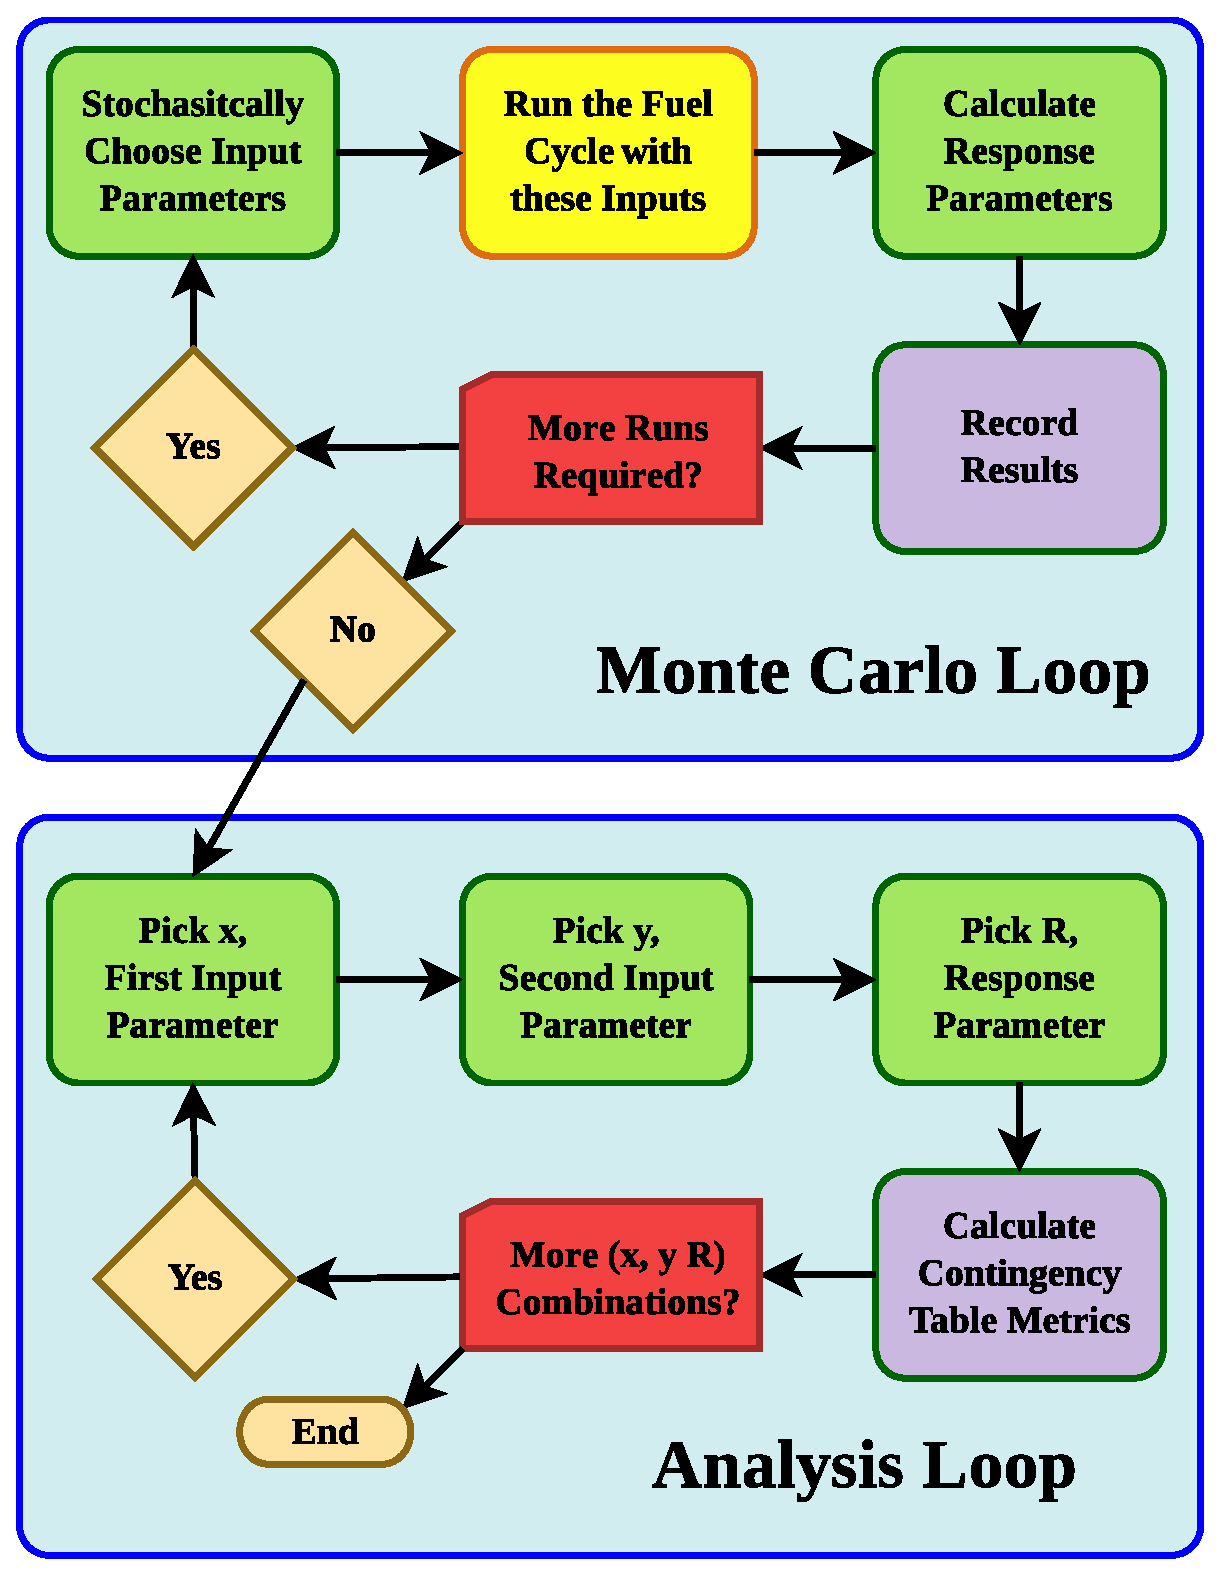
\includegraphics[scale=0.70]{ct_sensitivity/figs/MonteCarloMethodology.eps}
\caption{Monte Carlo Methodology \& Analysis Diagram}
\label{mcmethod}
\end{center}
\end{figure}

To further system analysis objectives, `standard' statistical metrics (such as the mean response
over all runs) may be calculated.  However, the usual correlation coefficients imply a linear
relationship between input and response.  Given the complexity of the system, linearity is not
a safe assumption for many system metrics.  Thus, novel information theoretic measures have
proved more valuable to ranking the importance of input parameters.

Additionally, it is useful to extend the information theoretic metrics from their typical 2D
formulations to the three dimensional equivalents.  If 3D metrics are constructed such that
they relate two input parameters to a response, then joint sensitivity or co-variance information
can be computed from a single set of stochastically-generated data.  Conditional covariances
(sensitivity of sensitivity) can thus be measured for two inputs to one response.
To maintain a realistic physical interpretation of this type of covariance, a combination of
entropy-based metrics extended to 3D metrics can be formulated  (discussed in section
\ref{sec:sensitivity_of_sensitivity_metrics}).  Any statistical analysis along these lines, though,
must be built around a model of the flow of materials through the nuclear fuel cycle, and the
transformations that constituent NFC technologies apply to the material flow.




\section{Nuclear Fuel Cycle Simulation}
\index{Nuclear Fuel Cycle Simulation@\emph{Nuclear Fuel Cycle Simulation}}
\label{cts_sec:nfcsim}

A fuel cycle simulation package that incorporates physics-based submodels of reactor burnup \cite{Scopatz2009} and
repository performance \cite{Li2009} served as the platform for this analysis. The approach taken in each
submodel is briefly summarized below. For additional details on this package refer to \cite{Li2009b}.

The importance of physics-based models (as opposed to curve fits or other parameterizations that are valid
only under specific conditions) in a sensitivity study of this type must be stressed. Given the number of
degrees of freedom associated with a fuel cycle scenario, it is not feasible, for example, to parameterize
reactor burnup with respect to transuranic isotopic stream compositions. Nor would it be possible to do
so for repository performance with respect to changes in host medium physical properties or system
geometry.

The reactor submodel couples burnup and criticality calculations \cite{Scopatz2009}. The burnup portion of the
model uses pre-tabulated physical data for each initially-present nuclide (neutron production and destruction
rates, burnup, and isotopic transformation) that are functions of fluence. These input curves are specific to a
given reactor and fuel type. The reactor model then uses mass-weighted superposition to recombine these
isotopic parameters as needed to calculate the multiplication factor and maximum discharge burnup. This result is
then folded in with a linear reactivity model for multi-batch criticality calculations that derive viable
fresh fuel compositions.

The repository thermal analysis model was developed based on the
analytical solution of a thermal conduction model for the presence of
loaded nuclear waste in a geologic repository \cite{Li2010a}. The
repository is modeled as a homogenous hosting medium with constant
properties. The nuclear waste packages were assumed to be loaded into parallel
waste emplacement drifts. Each drift is treated as
an infinite line heat source. The temperature increase at the critical
location is the superposition of temperature increase from each drift. The
undisturbed temperature field was assumed to be known, and the repository
capacity was determined according to the appropriate thermal design
constraints.



\subsection{Fuel Cycle Schema}
\index{Fuel Cycle Schema@\emph{Fuel Cycle Schema}}
\label{cts_sec:fcschema}

\begin{figure}[htbp]
\begin{center}
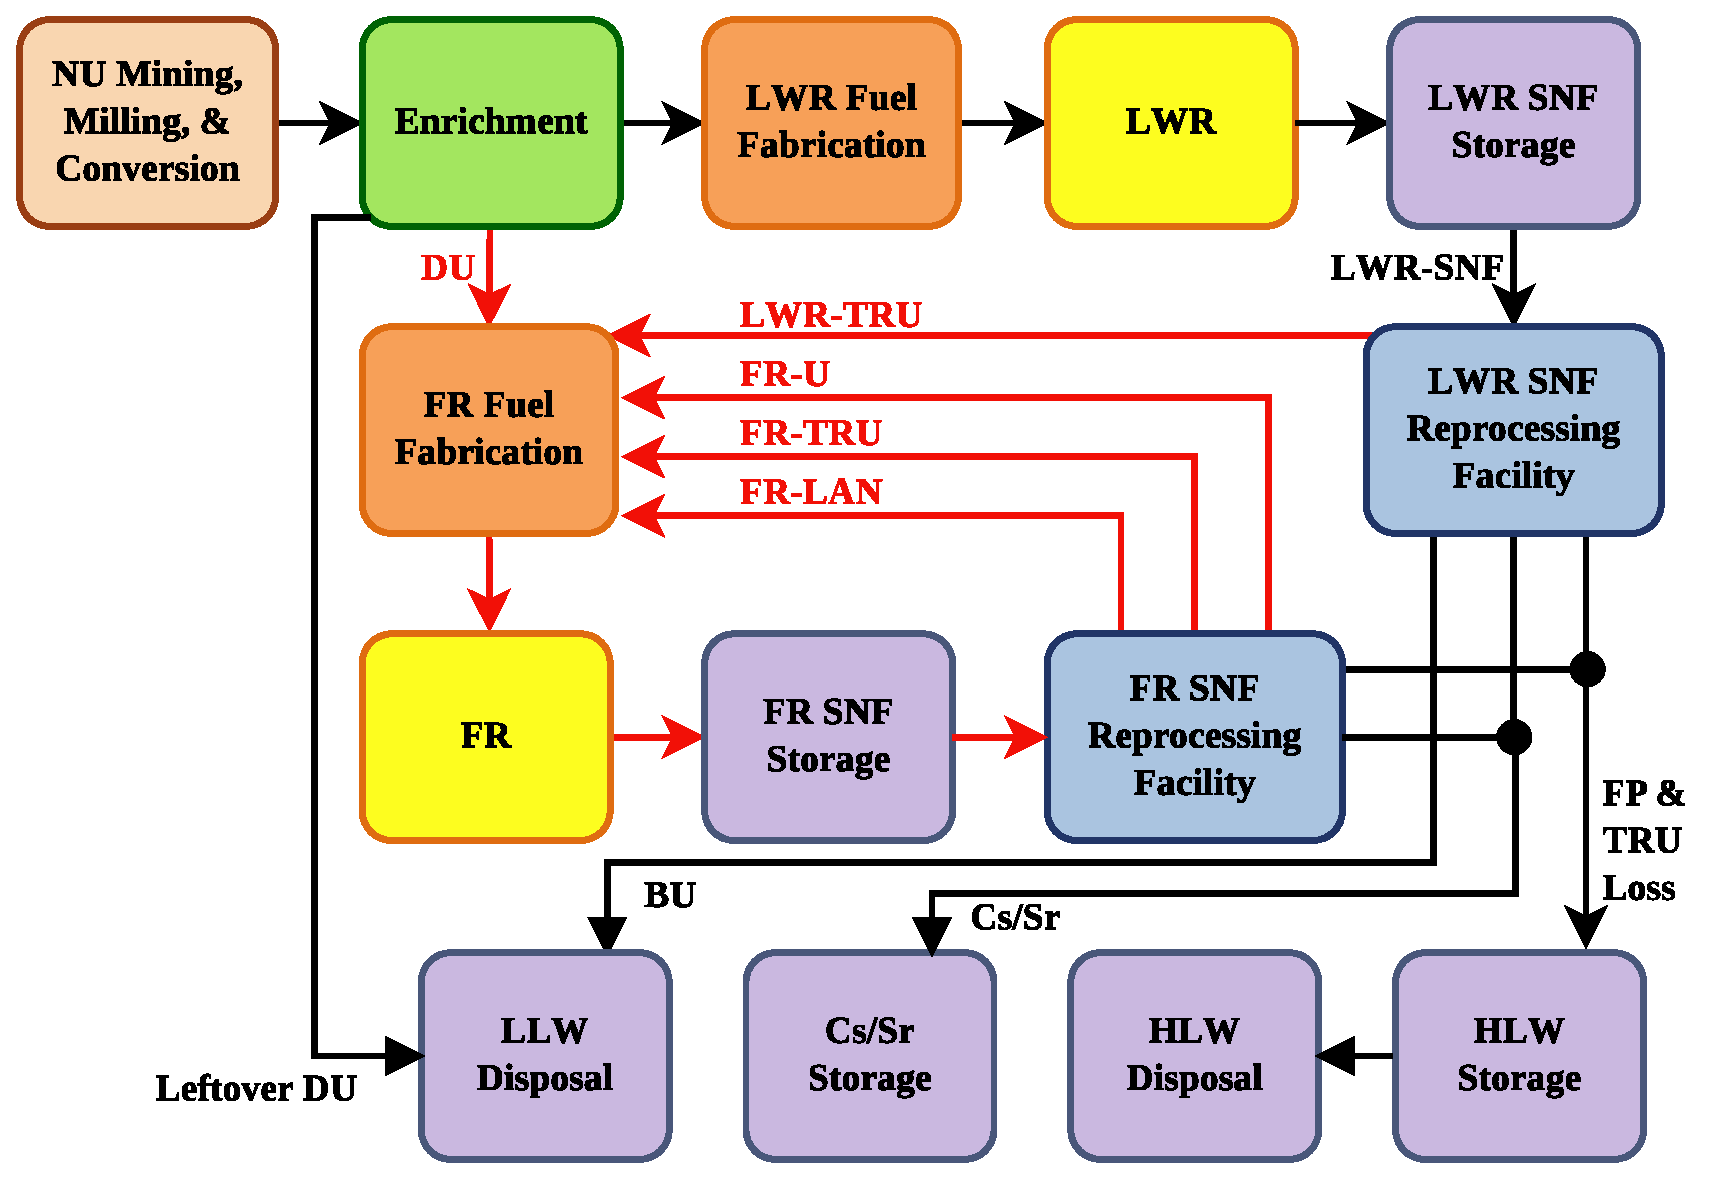
\includegraphics[scale=0.50]{figs/LWR_FR.eps}
\caption{LWR-FR Symbiotic Fuel Cycle Scenario}
\label{lwr_fr_fc}
\end{center}
\end{figure}

A sodium cooled fast burner (FR) - light water reactor (LWR) symbiotic cycle is studied here.
It is more fully detailed in \cite{Li2009b} and the corresponding flowchart
is seen in Figure \ref{lwr_fr_fc}. Although the model computes recycle passes
leading up to equilibrium \cite{Scopatz2009}, data (\emph{i.e.} the system wide performance
assessment metrics) are taken only after the fuel cycle has achieved its mass-balance equilibrium.
The statistical techniques discussed below could be applied to any type of fuel cycle; in this study,
the LWR and Na-cooled FR technologies were chosen for the fuel cycle simulation model
in order to strike a reasonable balance between input space richness, complexity, and familiarity to readers.

The fast reactors exist in support of the current and near-future
fleet of light-water reactors. The LWR used fuel (UF), after a cooling
period, is sent to an aqueous reprocessing facility. Here the transuranics (TRU) are separated out
from the fission products (FP) and
the burned uranium (BU).  The FP stream is further partitioned at the
LWR fuel reprocessing plant. The cesium and strontium are
separated out from the remaining FP. The Cs and Sr are
then emplaced in a storage facility built for medium-lived
isotopes while the BU goes to a low-level waste (LLW) disposal facility.
The remaining FPs and any losses from the other
streams (TRU, U, Cs/Sr) are treated as high-level waste (HLW) and sent to
the repository for permanent disposal.

Meanwhile, the recovered transuranics from the LWR
are mixed with depleted uranium (DU), and recycled FR
uranium and TRU. In this schema, all of the U and TRU
discharged from a FR (less reprocessing losses) are recycled into the fast reactor.
Thus the DU and LWR-TRU streams act as a top-up. By mixing in appropriate proportions (as
calculated in \cite{Scopatz2009}), new fuel for the fast reactors is
created.

After being re-burned in the FR, the used fuel once
again goes into cooling for three to thirty years. From here the fuel
is sent to a FR fuel reprocessing facility.  At the FR fuel reprocessing facility the actinide mass
of FR-UF is separated from the fission products present.
Again, the Cs and Sr are separated from the remaining FP.
The actinides are sent back to the fast reactor, the Cs/Sr
stream is disposed of in its own storage facility, and the
non-Cs/Sr fission products and losses from other streams
are sent to the deep geologic repository.  After reprocessing but prior to emplacement in 
the repository, the high level waste
stream is cooled for between one and three hundred years.
The deep geologic repository itself is modeled after
Yucca Mountain.



\subsection{Implementation}
\index{Implementation@\emph{Implementation}}
\label{cts_sec:implementation}

The fuel cycle model has been benchmarked against OECD and Idaho National Laboratory
(VISION) scenario analyses. When compared against the LWR-FR symbiotic cycle defined in Scheme
3a of the 2006 OECD fuel cycle system study \cite{NEA-5990}, agreement to within 5\% on the LWR-to-FR support
ratio and uranium and plutonium isotopics in the equilibrium mass flows was seen. Full benchmark
results are reported in \cite{Scopatz2009} and \cite{Li2009}.  For further details on this LWR-FR
symbiotic cycle refer to \cite{Shropshire2009}. The LWR and FR input parameters defined in
\cite{Shropshire2009} and reproduced in \cite{Scopatz2009} are points of departure for the
statistical analyses.

The physics-based methodology allows reactor performance and fuel cycle mass
balances to be rapidly recalculated under perturbations to design and operating 
parameters, where feedbacks to the operation of the cycle may have global reach.

\subsection{Parameter Specification}
\index{Parameter Specification@\emph{Parameter Specification}}
\label{cts_sec:paramspec}

Stochastic parameters are sampled either in a linearly uniform, log uniform, or one-minus-log uniform fashion.
The one-minus-log uniform distribution is useful for choosing separation efficiencies and is known as sampling
in the `nines'.  Table \ref{param_def} defines all thirty fuel cycle input parameters along with the six
responses computed by the model.  The scale column lists the sampling function
and the binning method implemented (see section \ref{sec:binning}) for each input parameter.

In the case where a set of input parameters is chosen such that the cycle is not physically calcuable,
internal variables inside of the models are adjusted to a point such that the fuel cycle is feasible.
For example, suppose a vector of inputs specifies a high value of the LWR burnup as well as other default
internal parameters.  The reactor model will adjust the non-leakage probability, the initial enrichment
of the fresh fuel, and the discharge fluence until these are tuned such that the stochastic burnup value
is obtained.

Thus every fuel cycle realization is its own distinct cycle, tuned for the stochastic parameters selected.
However, by bounding the input parameters and comparing many realizations, this study shows that the
output parameters are also bounded.  The spread of the output parameters due to changes in the inputs
determines the relative importance of that input.


%Input Variable Definition
\begin{table}
\caption{Fuel Cycle Parameter Definition}
\begin{center}
\scriptsize
\begin{tabular}{|l|l||c|c|c|c|}
\hline
\textbf{Input Parameter $x$} & \textbf{Abbreviation} & \textbf{Min} & \textbf{Max} & \textbf{Units} & \textbf{Scale}\\
\hline
LWR Burnup Level & \texttt{LWR\_BUd} & 30.0 & 80.0 & MWd/kgIHM & linear \\
\hline
LWR Fuel to Moderator Ratio & \texttt{LWR\_Fuel2Mod} & 0.28 & 0.36 & & linear \\
\hline
LWR UF Storage Time & \texttt{LWR\_UF\_Storage\_Time} & 3 & 30 & years & linear \\
\hline
SE of U from LWR UF & \texttt{LWR\_SE\_U} & 0.99 & 0.9999 & & nines \\
\hline
SE of NP from LWR UF & \texttt{LWR\_SE\_NP} & 0.9 & 0.9999 & & nines \\
\hline
SE of PU from LWR UF & \texttt{LWR\_SE\_PU} & 0.9 & 0.9999 & & nines \\
\hline
SE of AM from LWR UF & \texttt{LWR\_SE\_AM} & 0.9 & 0.9999 & & nines \\
\hline
SE of CM from LWR UF & \texttt{LWR\_SE\_CM} & 0.9 & 0.9999 & & nines \\
\hline
SE of CS from LWR UF & \texttt{LWR\_SE\_CS} & 0.9 & 0.9999 & & nines \\
\hline
SE of SR from LWR UF & \texttt{LWR\_SE\_SR} & 0.9 & 0.9999 & & nines \\
\hline
FR Burnup Level & \texttt{FR\_BUd} & 100.0 & 200.0 & MWd/kgIHM & linear\\
\hline
FR TRU Conversion Ratio & \texttt{FR\_TRU\_CR} & 0.25 & 0.95 & & linear \\
\hline
Lanthanide Fraction in FR Fresh Fuel & \texttt{FR\_LAN\_FF\_Cap} & 0.0001 & 0.005 & Atoms/TRU Atom & linear \\
\hline
FR UF Storage Time & \texttt{FR\_UF\_Storage\_Time} & 3 & 30 & years & linear \\
\hline
HLW Storage Time & \texttt{HLW\_Storage\_Time} & 1 & 300 & years & log \\
\hline
SE of U from FR UF & \texttt{FR\_SE\_U} & 0.99 & 0.9999 & & nines \\
\hline
SE of NP from FR UF & \texttt{FR\_SE\_NP} & 0.9 & 0.9999 & & nines \\
\hline
SE of PU from FR UF & \texttt{FR\_SE\_PU} & 0.9 & 0.9999 & & nines \\
\hline
SE of AM from FR UF & \texttt{FR\_SE\_AM} & 0.9 & 0.9999 & & nines \\
\hline
SE of CM from FR UF & \texttt{FR\_SE\_CM} & 0.9 & 0.9999 & & nines \\
\hline
SE of CS from FR UF & \texttt{FR\_SE\_CS} & 0.9 & 0.9999 & & nines \\
\hline
SE of SR from FR UF & \texttt{FR\_SE\_SR} & 0.9 & 0.9999 & & nines \\
\hline
Density of Host Rock & 2317 & \texttt{Rock\_Density} & 2869 & kg/m\superscript{3} & linear \\
\hline
Specific Heat of Host Rock & \texttt{Rock\_Specific\_Heat} & 590 & 1270 & J/kg-K & linear \\
\hline
Thermal Conductivity of Host Rock & \texttt{Rock\_Thermal\_Conductivity} & 1.9204 & 3.2856 & W/m-K & linear \\
\hline
Heat Loss Factor During Ventilation & \texttt{Heat\_Loss\_Factor} & 0.806 & 0.914 & & linear \\
\hline
Drift Diameter & \texttt{Drift\_Diameter} & 4.5 & 6.5 & m & linear \\
\hline
Ventilation System On Time & \texttt{Vent\_Stystem\_On\_Time} & 10 & 300 & years & log \\
\hline
Ambient Environment Temperature & \texttt{Ambient\_Temp} & 12.82 & 32.82 & C & linear \\
\hline
Distance Between Drifts & \texttt{Drift\_Space} & 56 & 106 & m & linear \\
\hline
\textbf{Response Parameter $R$} &  &  &  & & \\
\hline
Repository Capacity & \texttt{Capacity} & $10^4$ & $10^8$ & MTHM/Repository    & log \\
\hline
Fuel Cycle Cost  & \texttt{Cost} & 4.0    & 8.0    & \$/MWh             & linear \\
\hline
LWR-FR HLW Ratio  & \texttt{HLW\_Ratio} & 4.0    & 44.0   & gHM/GWh            & linear \\
\hline
LWR-FR Support Ratio  & \texttt{Support\_Ratio} & 0.0    & 3.0    & LWR cores/FR cores & linear \\
\hline
Total Electricity per Repository & \texttt{Total\_Electricity} & $5\times 10^8$ & $5\times 10^{12}$ & GWh/Repository & log \\
\hline
Toxicity Index & \texttt{Toxicity\_Index} & $10^6$ & $10^8$ & m\superscript{3}/MTHM & log \\
\hline
\end{tabular}
\end{center}
\label{param_def}
\end{table}




\section{Contingency Tables}
\index{Contingency Tables@\emph{Contingency Tables}}
\label{cts_sec:ct}

After the stochastic generation of set of input parameters, the analysis loop of Figure \ref{mcmethod} is entered.
Since all inputs are varied simultaneously, the response from single input parameter is implicitly
a function of all other inputs as well.  With thirty inputs, all outcomes exist in a 31 dimensional space.

Therefore, if a deterministic sampling approach were used and one hundred points
were chosen per input parameter, then $10^{60}$ fuel cycle realizations would be 
needed to have full coverage over all space.

Hence the stochastic method achieves much better coverage much faster.  However, 
even one hundred thousand points may not \emph{a priori} be enough.  A mechanism 
for measuring the quality of the data will be discussed in section \ref{sec:binning}.

Contingency tables (CT) \cite{Everitt1992} \cite{Press2007} \cite{Yao2003} \emph{associate} two parameters of a
complex system in a way that is independent of the functional form of the actual system.
Given that CTs have a rich history of their own, the authors seek not to fully characterize them.  
Rather, this paper presents the use of contingency tables as a fuel cycle performance assessment tool.

A simple example illustrates the CT concept valuable to understanding the following analyses.  For a 
fictitious sample population, a biologist may be interested in the correlation between hair color and sex.  
They might then set up a $2\times 2$ tabulation similar to Table \ref{biotable}.  Structurally, the matrix of 
data itself sits in the center, while marginal sums are displayed along the right and bottom.

\begin{table}[htbp]
\begin{center}
\caption{Hair Color to Sex Contingency Table}
\label{biotable}
\begin{tabular}{|l||c|c||c|}
\hline
       & Blonde & Brunette & Totals \\
\hline
Female & 18     & 17       & 35 \\
\hline
Male   & 11     & 14       & 25 \\
\hline
Totals & 29     & 31       & 60 \\
\hline
\end{tabular}
\end{center}
\end{table}

Of note for Table \ref{biotable} is that both sex and hair color can be interpreted as responses to 
underlying human biological mechanisms.  Since the body is being treated as a black box, contingency 
tables do not distinguish between input and output parameters.

Additionally, Table \ref{biotable} uses categorical, discrete variables.  However, CTs may also be 
implemented using data that is a function of a continuous real variable, equally partitioned on the scale of
interest. For instance, exponential data could have one bin per decade.

For the NFC and input parameter family considered here, all parameters are functions of a real 
(stochastic) continuous variable.  This approach can support discrete variables too (e.g., a 
boolean flag indicating the availability of mixed-oxide fuel), but that avenue is not developed 
in this study. For the continuous variables, more than two bins are required to
be able to demonstrate a meaningful association.  It will be shown that 7 bins per axis on the 
contingency tables give rise to acceptable
statistical fidelity.  However, even seven bins becomes unwieldy for visualization.
Table \ref{ct2d_example} displays a $4\times 3$ fuel cycle CT from the data set computed in
the Monte Carlo loop.   This example compares the FR plutonium separation efficiency (SE) to the 
repository capacity, irrespective of what the values the other 29 system inputs take on.

\begin{table}
\caption{Contingency Table for FR Plutonium SE to Repository Capacity [MTHM/Repository].}
\begin{center}
\tiny
\begin{tabular}{|c||c|c|c||c|}
\hline
&$0.9<$\texttt{SE}$<0.99$&$0.99<$\texttt{SE}$<0.999$&$0.999<$\texttt{SE}$<0.9999$&\\
\hline
$10^4 <$ \texttt{Capacity} $< 10^5$&$739$&$43$&$27$&$809$\\
\hline
$10^5 <$ \texttt{Capacity} $< 10^6$&$31510$&$21611$&$19469$&$72590$\\
\hline
$10^6 <$ \texttt{Capacity} $< 10^7$&$2648$&$13095$&$14430$&$30173$\\
\hline
$10^7 <$ \texttt{Capacity} $< 10^8$&$0$&$213$&$1053$&$1266$\\
\hline
&$34897$&$34962$&$34979$&$104838$\\
\hline
\end{tabular}
\end{center}
\label{ct2d_example}
\end{table}


The zero entry in Table \ref{ct2d_example} implies that for low plutonium separation efficiencies 
a high repository capacity is impossible.
Additionally, some regions arise rarely, assumedly only for extreme values of one or more other inputs.
High plutonium SE and low repository capacities occur with a vanishingly
small probability.  The combination of these two restricted regimes leads to a table that is 
largely banded down the diagonal.
The statistical measures chosen for examination should capture these effects.

As mentioned previously, contingency tables are not restricted to a two-way formulation.  
Three dimensional tables may also be constructed from the same
fuel cycle realizations.  In an effort to capture co-variant system effects, this paper 
examines two independent parameters ($x$ and $y$) and one response ($R$).  For instance, 
if the SE of plutonium coming from the FR changes, it is expected that the relative benefit 
from the HLW storage period will also change.
Thus the repository capacity must be expressed as a combination of these two parameters together.

\begin{center}
\begin{table}[htbp]
\caption{3D Contingency Table Relating FR Plutonium SE and the HLW Storage Time [years] to the Repository Capacity [MTHM/Repository].}
\label{ct3d_example}
\begin{center}
\begin{tabular}{|c||c|c|c||c|}
\hline
\multicolumn{5}{|c|}{Slice for 1 $<$ \texttt{HLW\_Storage\_Time} $<$ 6.694}\\
\hline
&$0.9 <$ \texttt{SE} $< 0.99$&$0.99 <$ \texttt{SE} $< 0.999$&$0.999 <$ \texttt{SE} $< 0.9999$&\\
\hline
$10^4 <$ \texttt{Capacity} $< 10^5$&$419$&$23$&$14$&$456$\\
\hline
$10^5 <$ \texttt{Capacity} $< 10^6$&$11145$&$9970$&$9553$&$30668$\\
\hline
$10^6 <$ \texttt{Capacity} $< 10^7$&$110$&$1556$&$2085$&$3751$\\
\hline
$10^7 <$ \texttt{Capacity} $< 10^8$&$0$&$0$&$0$&$0$\\
\hline
&$11674$&$11549$&$11652$&$34875$\\
\hline
\hline
\multicolumn{5}{|c|}{Slice for 6.694 $<$ \texttt{HLW\_Storage\_Time} $<$ 44.814}\\
\hline
&$0.9 <$ \texttt{SE} $< 0.99$&$0.99 <$ \texttt{SE} $< 0.999$&$0.999 <$ \texttt{SE} $< 0.9999$&\\
\hline
$10^4 <$ \texttt{Capacity} $< 10^5$&$273$&$19$&$11$&$303$\\
\hline
$10^5 <$ \texttt{Capacity} $< 10^6$&$10859$&$7527$&$6373$&$24759$\\
\hline
$10^6 <$ \texttt{Capacity} $< 10^7$&$484$&$4157$&$5175$&$9816$\\
\hline
$10^7 <$ \texttt{Capacity} $< 10^8$&$0$&$2$&$24$&$26$\\
\hline
&$11616$&$11705$&$11583$&$34904$\\
\hline
\hline
\multicolumn{5}{|c|}{Slice for 44.814 $<$ \texttt{HLW\_Storage\_Time} $<$ 300}\\
\hline
&$0.9 <$ \texttt{SE} $< 0.99$&$0.99 <$ \texttt{SE} $< 0.999$&$0.999 <$ \texttt{SE} $< 0.9999$&\\
\hline
$10^4 <$ \texttt{Capacity} $< 10^5$&$47$&$1$&$2$&$50$\\
\hline
$10^5 <$ \texttt{Capacity} $< 10^6$&$9506$&$4114$&$3543$&$17163$\\
\hline
$10^6 <$ \texttt{Capacity} $< 10^7$&$2054$&$7382$&$7170$&$16606$\\
\hline
$10^7 <$ \texttt{Capacity} $< 10^8$&$0$&$211$&$1029$&$1240$\\
\hline
&$11607$&$11708$&$11744$&$35059$\\
\hline
\hline
\multicolumn{5}{|c|}{Summary for summation over HLW\_Storage\_Time}\\
\hline
&$0.9 <$ \texttt{SE} $< 0.99$&$0.99 <$ \texttt{SE} $< 0.999$&$0.999 <$ \texttt{SE} $< 0.9999$&\\
\hline
$10^4 <$ \texttt{Capacity} $< 10^5$&$739$&$43$&$27$&$809$\\
\hline
$10^5 <$ \texttt{Capacity} $< 10^6$&$31510$&$21611$&$19469$&$72590$\\
\hline
$10^6 <$ \texttt{Capacity} $< 10^7$&$2648$&$13095$&$14430$&$30173$\\
\hline
$10^7 <$ \texttt{Capacity} $< 10^8$&$0$&$213$&$1053$&$1266$\\
\hline
&$34897$&$34962$&$34979$&$104838$\\
\hline
\end{tabular}
\end{center}
\end{table}
\end{center}





Table \ref{ct3d_example} has a $4\times 3\times 3$ bin structure relating the $R$ response 
to $x$ \& $y$ inputs.  Here, it is essential to note that every $y$ bin
is itself a 2D contingency table for $x$ to $R$.
Additionally, the bottom slice in Table \ref{ct3d_example} represents the marginal sums over 
the $y$ axis.  Because $x$ here was chosen the same as in the
2D case (\texttt{FR\_SE\_PU}), the last slice in Table \ref{ct3d_example} \emph{is} Table 
\ref{ct2d_example}.  Therefore the 2D CT for \texttt{HLW\_Storage\_Time}
to \texttt{Capacity} is represented by the right-hand column of Table \ref{ct3d_example}.
Since there are thirty inputs, of which two are examined, there are $_{30}C_2 = 435$ three 
dimensional contingency tables that may be constructed for every response.


\subsection{Statistical Metrics}
\index{Statistical Metrics@\emph{Statistical Metrics}}
\label{cts_sec:statistical_metrics}

This section describes the statistical measures used to quantify the strength of association 
between input parameters and responses in contingency tables.
This allows the system designer to determine the most `important' input parameters to this response.  
For example, one
could quantitatively state the degree of importance of FR plutonium SE relative to the repository drift 
diameter in the sense of how each affects the repository capacity.

\subsubsection{Entropy}
\index{Entropy@\emph{Entropy}}
\label{cts_sec:entropy}

The \emph{entropy} $H$ of a parameter or CT is a measure of how evenly spread out the data is over all 
bins.  This metric can be thought of
in analogy to the thermodynamic property of the same name.  For contingency tables,
maximum entropy implies that all entries in the table have exactly the same value.
Conversely, zero entropy implies a fully ordered system.  In contingency tables, zero entropy implies 
that every row and every column have exactly one
non-zero entry.  All independent input parameters $x$ should have maximum entropy since they are 
randomly sampled.

To calculate the entropy, the probability table corresponding to the CT is needed.  If there are $N$ 
total Monte Carlo runs, then any bin in
the contingency table may be represented by the matrix element $N_{ab}$.  Here $a$ indexes the number 
of response bins $A$, while $b$
indexes the number of $x$ input parameter bins $B$.  For the three dimensional table, $N_{abc}$ 
represents a matrix element where $c$ indexes the number of $y$
input parameter bins $C$.  Thus the probability table may be defined such that:
\begin{equation} p_{ab} = \frac{N_{ab}}{N} \, \forall a, b\in A\times B\end{equation}
Additionally, marginal sums are represented by a subscript dot notation.  The `dotted' index or 
indices are the rows or columns that are summed over.  For example,
\begin{equation} p_{\cdot b} = \sum_a^A p_{ab} \end{equation}
\begin{equation} N = N_{\cdot \cdot} = \sum_{a,b}^{A,B} N_{ab} \end{equation}
Then, the entropy is defined as the sum of $p\log p$ for any parameter or parameter combination:
\begin{equation} H(R) = - \sum_a^A p_{a \cdot} \ln(p_{a \cdot}) \end{equation}
\begin{equation} H(x) = - \sum_b^B p_{\cdot b} \ln(p_{\cdot b}) \end{equation}
\begin{equation} H(R,x) = - \sum_{a,b}^{A,B} p_{ab} \ln(p_{ab}) \end{equation}
The last entropy in the equations above, $H(R,x)$, is known as the \emph{joint entropy} since 
it measures the entropy of the contingency table as a whole.
Three dimensional expressions for entropy may be extrapolated from the equations above.

Entropy is not neatly bounded on the range $[0,1]$.
Rather the maximum value for the entropy is given as the natural logarithm of the total 
number of bins $K$ of any table or slice such that
the entropy is defined on the range $[0, \ln(K)]$.

\subsubsection{Mutual Information}
\index{Mutual Information@\emph{Mutual Information}}
\label{sec:mutual_information}

The next metric is the \emph{mutual information} $I$.
The mutual information is defined as the overlap in the entropies of various parameters.
Figure \ref{entropy_info_relations} displays the relationship between the various entropies 
and the mutual information graphically.
This figure is based on a similar one presented in \cite{Press2007}.
\begin{figure}
\caption{Relationship between the Mutual Information and Entropy \cite{Press2007}}
\begin{center}
\setlength{\unitlength}{1.5cm}
%\begin{picture}(9,3)(-4.5,-1.5)
\begin{picture}(9,2)(-4.5,0.0)
\thicklines
\put(0,1.5){\vector(1,0){4.5}}
\put(0,1.5){\vector(-1,0){4.5}}
\put(-0.7,1.2){$H(x,R)$}

\put(-2.25,1.0){\vector(1,0){2.25}}
\put(-2.25,1.0){\vector(-1,0){2.25}}
\put(-2.6,0.7){$H(x)$}

\put(1.5,0.5){\vector(1,0){3}}
\put(1.5,0.5){\vector(-1,0){3}}
\put(1.2,0.2){$H(R)$}

\put(-0.75,0){\vector(1,0){0.75}}
\put(-0.75,0){\vector(-1,0){0.75}}
\put(-1.2,-0.3){$I(R,x)$}

\end{picture}
\end{center}
\label{entropy_info_relations}
\end{figure}
As a physical example, consider the DNA sequences of a parent and a child.  The sequence of 
the child ($R$) is some unknown function of the DNA of the parent ($x$).
$I(R,x)$ then measures the overlap of the sequences, in entropy space.

The mutual information indicates how much of a response is determined by a particular input.
As an illustration, FR UF separations might account for half of the variation in fuel cycle costs.  
However, FR burnup may also
account for half of the variability.  Yet, these halves likely have a significant overlap since both 
affect the amount of TRU top-up required on the next pass.
The maximum possible overlap could be inferred by comparing the mutual information values for each of 
these two inputs.

The mutual information may be calculated in two- and three-dimensional senses as follows:
\begin{equation}
I(R,x) = - \sum_{a,b}^{A,B} p_{ab} \ln\left(\frac{p_{ab}}{p_{a\cdot}\cdot p_{\cdot b}}\right) 
\end{equation}
\begin{equation}
I(R,x,y) = - \sum_{a,b,c}^{A,B,C} p_{abc} \ln\left(\frac{p_{abc}}{p_{a\cdot \cdot}\cdot p_{\cdot b \cdot}\cdot p_{\cdot \cdot c}}\right)
\end{equation}
The minimum value of $I$ is zero, indicating that $x$ and $R$ share nothing in common.  
This occurs when $x$ and $R$ are fully independent.
On the other hand, the maximum value of the mutual information depends on the structure 
of the contingency table and may not be easily expressed in general.





\subsubsection{Uncertainty}
\index{Uncertainty@\emph{Uncertainty}}
\label{cts_sec:uncertainty}

The uncertainty $U$ is the first metric to be used to rank the relative value of input 
parameters to a response.  Informally, the uncertainty is defined
as the mutual information divided by the entropy.

More exactly, the \emph{uncertainty coefficients} are used to rank inputs.  They are 
specified with the conditional notation $U(x|R)$.  Such coefficients are calculated via:
\begin{equation}
U(x|R) = \frac{I(R,x)}{H(x)}
\label{eq:U_x_R}
\end{equation}
In essence, equation \ref{eq:U_x_R} measures the extent to which knowing the input $x$ 
is the same as knowing the response $R$.  As such, $U(x|R)$ has the following properties:
\begin{enumerate}
    \item Defined on the range $[0, 1]$.
    \item $U(x|R) = 0$ implies that $I(R,x) = 0$, which indicates that the parameter
        is unassociated with the response.
    \item $U(x|R) = 1$ requires that $I(R,x) = H(x)$.  This implies that
        the system response $R(x)$ is solely determined by $x$.
\end{enumerate}

It is important to note that both $H(R)$ and $H(x)$ are the same for all $x$.  Thus the 
rankings of $x$ from $U(x|R)$ are the same as the rankings from the, perhaps more natural, 
uncertainty coefficient $U(R|x)$.  Hence, the scaling factor, seen in equation 
\ref{uncertainty_scale}, is the same for all inputs.
\begin{equation}
U(x|R) = \frac{H(R)}{H(x)} U(R|x)
\label{uncertainty_scale}
\end{equation}

Moreover, a related uncertainty coefficient may be calculated for the three dimensional 
case of two inputs to one
response.  $U(x,y|R)$ is computed from:
\begin{equation} U(x,y|R) = \frac{I(R,x,y)}{H(x,y)} \end{equation}
The reason for choosing $U(x,y|R)$ as opposed to $U(R|x,y)$ follows analogously to the 
two dimensional case.

In fact, the interpretation of $U(x,y|R)$ is much the same as the meaning of $U(x|R)$.  
The difference here is that input parameter pairs are being compared to
all other $(x, y)$ combinations.  For instance, by ranking with this 3D metric, the fuel 
cycle analyst may quantitatively state that the FR plutonium and americium SEs
together are more important to the repository capacity than the repository drift diameter 
together with the LWR neptunium SE.


\subsubsection{Sensitivity of Sensitivity Metrics}
\index{Sensitivity of Sensitivity Metrics@\emph{Sensitivity of Sensitivity Metrics}}
\label{cts_sec:sensitivity_of_sensitivity_metrics}

In so far as the uncertainty coefficient is a surrogate for sensitivity, a suitable 
replacement for covariance should be found.
This sort of association is called a \emph{sensitivity of sensitivity} because it seeks
to quantify the sensitivity of $x$ given the sensitivity of  $y$ to the response $R$.

To obtain such a metric, recall that each slice of a three-way table is itself a 2D contingency table.  
It is therefore possible to compute the uncertainty
coefficient $U(x|R)$ for every slice over $y$.  In doing so, a set of $C$ uncertainties are generated 
such that,
\begin{equation}
\label{eq:U_x_R_y}
U(x|R)|y = \left\{ \left.U(x|R)\right|_{l_0}^{l_1}, \left.U(x|R)\right|_{l_1}^{l_2}, \ldots \left.U(x|R)\right|_{l_{C-1}}^{l_C}  \right\}
\end{equation}
where $l$ is a sequence of $C+1$ points that defines the bin boundaries of $y$.
From here, the mean $\mu$ and standard deviation $\sigma$ of the set seen in equation \ref{eq:U_x_R_y} may be 
calculated.
\begin{equation}
\mu(U(x|R)|y) = \frac{1}{C} \sum_c^C U(x|R)|y_c 
\end{equation}
\begin{equation}
\sigma(U(x|R)|y) = \sqrt{ \frac{1}{C} \sum_c^C \left( U(x|R)|y_c - \mu(U(x|R)|y) \right)^2 } 
\end{equation}
However, the choice of slicing along $y$ is somewhat arbitrary.  One could instead slice along $x$ 
and compute $\mu(U(y|R)|x)$ and $\sigma(U(y|R)|x)$
by analogy to the equations above.

Dividing the standard deviation by the mean yields a \emph{coefficient of variation} $c_v$:
\begin{equation} c_v(U(x|R)|y) = \frac{\sigma(U(x|R)|y)}{\mu(U(x|R)|y)} \end{equation}
Unlike the uncertainty coefficient, $c_v(U(x|R)|y)$ is not symmetric with respect to $x$ and $y$.  
Thus the same pair will have a different rank when measuring
with $c_v(U(y|R)|x)$.  A symmetric expression of the coefficient of variation is obtained by taking 
the average of the non-symmetric terms:
\begin{equation}
c_v(x|y|R) = \frac{1}{2} \left(c_v(U(x|R)|y) + c_v(U(y|R)|x)\right)
\end{equation}
This measure has the following properties:
\begin{enumerate}
    \item Defined on the range $[0, 1]$ since $0 \le U \le 1$.
    \item $c_v = 0$ implies that both $\sigma = 0$, which indicates that $U(x|R)$
        shows no dependence on $y$.  Thus there are no covariant effects observed.
    \item $c_v = 1$ indicates that both $\sigma = \mu$.  This connotes
        that the value of $x$ soley governs the response $R$ from $y$.
\end{enumerate}

The difference in ranking parameter pairs using $U(x,y|R)$ versus $c_v(U(x|R)|y)$ is that the uncertainty 
coefficient measures the magnitude of the effect on $R$ while the coefficients of variation measure the 
interdependence of $x$ and $y$ on the response. For example, the HLW storage time together with the LWR UF 
storage time are not of global importance to the repository capacity (low $U(x,y|R)$ value).
However, changing one input has a great effect on the impact of other input to the repository capacity 
(high $c_v$ value). Therefore, both metrics are needed to have a complete description of the three 
dimensional contingency tables.



\section{Results \& Case Studies}
\index{Results \& Case Studies@\emph{Results \& Case Studies}}
\label{cts_sec:results}

The goal of this study, similar to other sensitivity studies \cite{Scopatz2010b} or uncertainty 
analyses \cite{Barratt2004}, is to quantitatively rank fuel cycle inputs against their effect on 
the chosen response.  Here, the two dimensional uncertainty $U(x|R)$ takes the place of a 
traditional sensitivity.  Likewise, the three dimensional $U(x,y|R)$ may be seen as a sensitivity 
for a pair of parameters.  Lastly, the coefficient of variation $c_v(U(x|R)|y)$ is taken as a 
measure of covariance effects between $x$ and $y$.  The covariance metric shows that some parameter 
pairs have a significant joint effect on the fuel cycle. Hence, $x$ and $y$ may exhibit a greater 
(or less than) commensurate response on the fuel cycle response than the sum of $x$ and $y$ 
effects individually.


A brief examination of the binning structure and how it was determined is follows. 
Then, an illustration of the rankings of all fuel cycle metrics for the 2D \& 3D sensitivities 
and covariant analyses is presented.  The final portion of this section reviews case studies 
about particular parameters and pairs of interest.


\subsection{Binning Structure}
\index{Binning Structure@\emph{Binning Structure}}
\label{cts_sec:binning}

Inevitably when performing Monte Carlo calculations the question of `good statistics' arises.  
At the root of this question is the concern that enough runs
have been performed to ensure that the subsequent analysis can be made with confidence. 

Moreover, contingency tables exhibit dynamic effects as a function of the number of bins used to 
generate them, even for the same underlying data set.  An example from
thermodynamics demonstrates this behavior.  Take a chamber the moment after a piston has been 
suddenly removed, as in a Carnot heat engine.
This system is not at its highest entropy.  Most of its fluid lies in the part of the chamber 
that was not compressed by the piston while most of the
chamber remains evacuated.

\begin{figure}[htbp]
\begin{center}
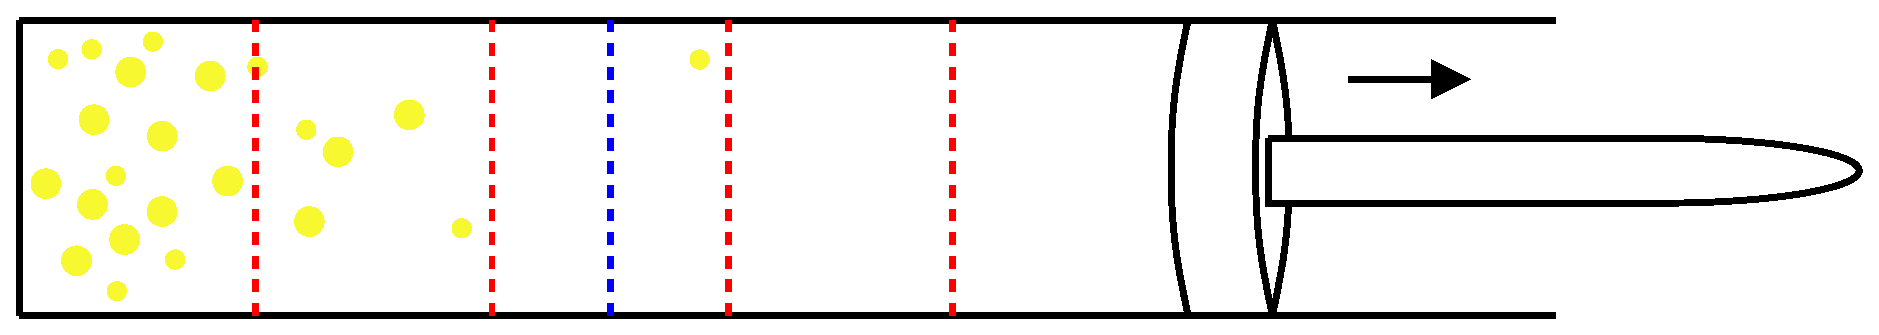
\includegraphics[scale=0.50]{ct_sensitivity/figs/PistonCT.eps}
\caption{Abstract Piston with Representative Partitions: Blue Line for 2 Bins, Red Line for 5 Bins.}
\label{piston_ct}
\end{center}
\end{figure}

Now, to capture the state of the piston, impose imaginary partitions at equidistant points in the 
chamber.  A diagram of this is seen in Figure \ref{piston_ct}.  The blue
dotted line represents partitioning the piston chamber into two distinct bins.  The particle 
distribution is heavily weighted to the leftmost bin
since this is where the large majority of the fluid (yellow dots) falls.  

The red dotted lines in Figure \ref{piston_ct} represent the same chamber partitioned into 
five bins.  The left most red partition runs through the
densely populated region, adding information about the distribution that was not available 
under the more corasely-binned structure.

From this one might conclude that only an infinite number of partitions and bins would converge 
to the `true' value of the entropy.  However, this is not necessary for contingency tables.  
The metrics (entropy, uncertainty, \emph{et cetera}) rely on the relative populations of the bins.
An infinite number of partitions would result in zero or one particle per bin, thereby 
giving in poor statistics.

Thus there is a balancing act between the number of bins and the number of stochastic 
simulation executions.  This study uses a symmetric seven bins per axis formulation.  
(Two dimensional tables have $7^2=49$ bins while the three dimensional tables have
$7^3=343$ bins.)
Such behavior is consistent with other Monte Carlo techniques \cite{Press2007}.

\begin{figure}[htbp]
\begin{center}
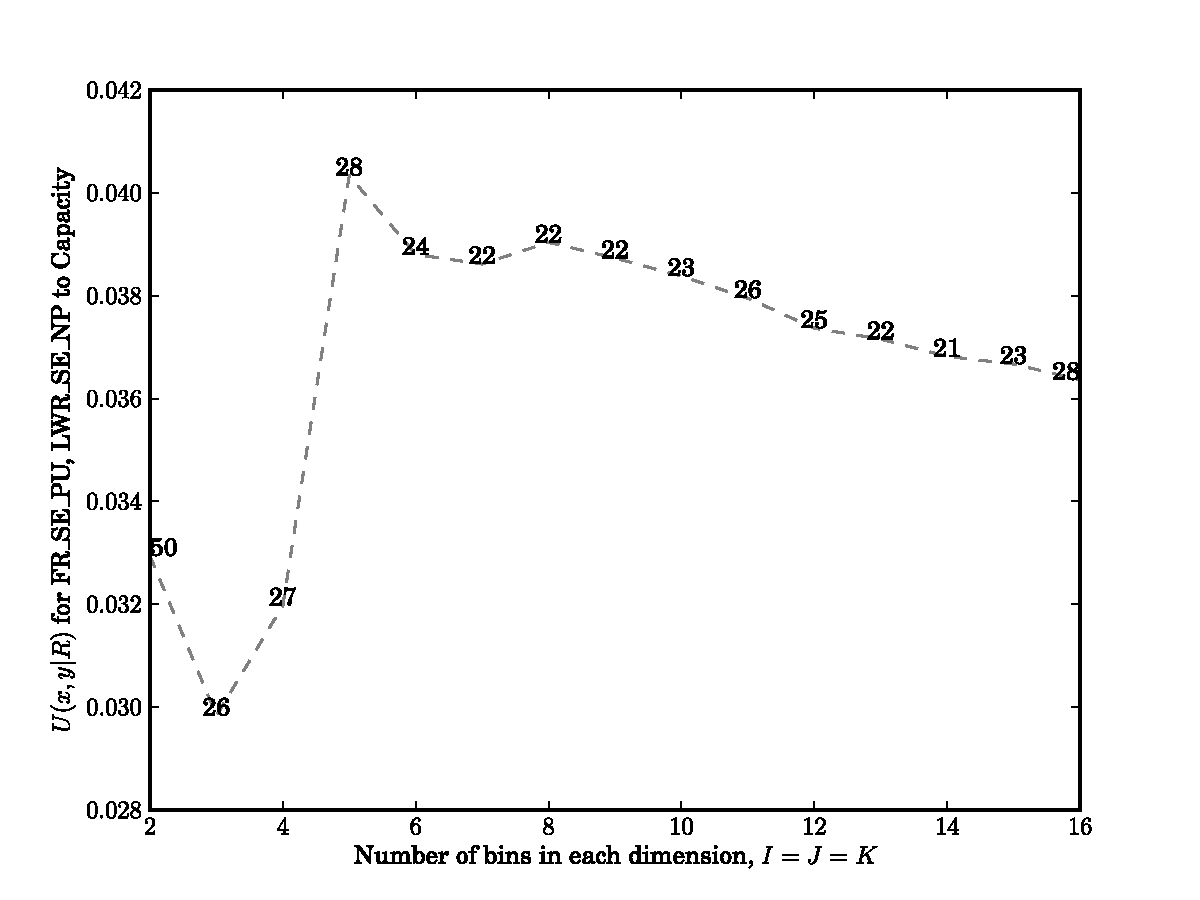
\includegraphics[scale=0.70]{ct_sensitivity/figs/U_xy_R_for_FR_SE_PU_and_LWR_SE_NP_to_Capacity_rank.eps}
\caption{Dynamic Effects of Binning Structure Example: $U(x,y|R)$ for the parameter pair (\texttt{FR\_SE\_PU}, \texttt{LWR\_SE\_NP}) to repository capacity.}
\label{dynamic_effects}
\end{center}
\end{figure}

Seven bins per axis were chosen since the uncertainty rankings for moderately important 
parameter pairs stabilize at approximately this point.  While the choice of binning 
resolution is system-specific -- it depends on the dynamics of the underlying 
simulation model -- important parameters are always going to dominate the top 
ranks and non-important ones will change ranks rapidly, but randomly.  Therefore 
it is necessary  to examine the parameters which are most sensitive to the binning effects.

Figure \ref{dynamic_effects} shows how the 3D sensitivity $U(x,y|R)$ for FR 
plutonium separation efficiency and LWR neptunium separation efficiency given the repository
capacity changes as a function of symmetric bin structure (\emph{i.e.} $A=B=C$).  
It is known that \texttt{FR\_SE\_PU} is very important
while \texttt{LWR\_SE\_NP} is not.  Therefore the combination of these two inputs 
has some modest impact largely driven by the plutonium vector.

Figure \ref{dynamic_effects} displays both the value of the uncertainty metric 
for this parameter pair as well as its relative ranking to all other pairs.
Lower ranks ($1, 2, \ldots$) indicate more important parameters while higher 
ranks ($\ldots, 29, 30$ or $\ldots, 434, 435$) mean that the parameter has less overall
impact.  From this figure, the importance of (\texttt{FR\_SE\_PU}, \texttt{LWR\_SE\_NP}) 
fluctuates significantly from 50 to the mid-twenties for low symmetric
bin number.  However once 7 bins are reached, the rank stabilizes at ~22.  This stability 
indicates that the repository capacity response to changes in \texttt{FR\_SE\_PU} and 
\texttt{LWR\_SE\_NP}, relative to the response for similarly important parameter pairs, 
becomes well-captured at 7-bin resolution.

After 10 bins, the rank creeps up and down.  This is expected as the number of
fuel cycle realizations remains constant for all bin numbers.  Thus higher bin numbers 
relate to correspondingly worse statistics for the contingency table (see below).  
The goal, therefore, is to pick the lowest bin number after which the rankings have 
become stable.  Such a point for this study seems to lie at approximately
7 bins per axis.  Studies have been made of several other parameter pairs to support this conclusion.

The mutual information may be used to ensure that the binning structure offers 
satisfactory statistics given the number of stochastic realizations available.  
Since every input parameter is independent of every other input parameter, $I(x,y)$ 
should be zero for all combinations of $x$ and $y$
in the limit as $N$ becomes large.

Call $t$ the maximum acceptable tolerance along any stochastic axis.
For instance, $t = 0.01$ indicates a 1\% intrinsic uncertainty.
Then the threshold mutual information for `good' statistics goes as $I(x,y) \approx t^2$, since
two stochastic parameters are being compared.  The approximate number of runs required to achieve $t$ is thus:
\begin{equation}
\label{runs_needed}
N \approx \frac{1}{t^2} B C
\end{equation}
Thus by equation \ref{runs_needed}, it is a factor of $25$ times easier to achieve 5\% 
uncertainty than to get to the 1\% level for the same binning structure.
Given $100,000$ runs performed here and seven bins on each axis, equation \ref{runs_needed} implies
that the induced uncertainty is approximately 2.2\%.  Seven bins per axis are used for the 
remainder of this analysis.



\subsection{Rankings: One Input to One Response}
\index{Rankings: One Input to One Response@\emph{Rankings: One Input to One Response}}
\label{cts_sec:rank2D}

Determining the impact of a single input parameter on a nuclear fuel cycle outcome is the 
first step in a screening study.  Using the contingency table methodology above,
the uncertainty coefficient $U(x|R)$ measures the importance of $x$.  
Table \ref{U_x_R_for_Capacity_with_IJK7} displays the input parameters, ranked by
uncertainty, for the repository capacity response.

\begin{center}
\begin{table}[htbp]
\caption{Input Parameters Ranked by $U(x|R)$ for \texttt{Capacity} [MTHM/Repository]}
\label{U_x_R_for_Capacity_with_IJK7}\begin{center}
\begin{tabular}{|r|l|c|}
\hline
Rank&\textbf{$x$}&\textbf{$U(x|R)$}\\
\hline
1&\texttt{FR\_SE\_PU}&0.07667\\
\hline
2&\texttt{HLW\_Storage\_Time}&0.05264\\
\hline
3&\texttt{FR\_SE\_AM}&0.04148\\
\hline
4&\texttt{Heat\_Loss\_Factor}&0.01548\\
\hline
5&\texttt{LWR\_SE\_PU}&0.01343\\
\hline
6&\texttt{FR\_TRU\_CR}&0.008895\\
\hline
7&\texttt{LWR\_SE\_AM}&0.007304\\
\hline
8&\texttt{FR\_BUd}&0.003773\\
\hline
9&\texttt{LWR\_SNF\_Storage\_Time}&0.003551\\
\hline
10&\texttt{Rock\_Specific\_Heat}&0.003085\\
\hline
11&\texttt{FR\_SE\_CM}&0.002522\\
\hline
12&\texttt{Rock\_Thermal\_Conductivity}&0.001954\\
\hline
13&\texttt{Ambient\_Temp}&0.001353\\
\hline
14&\texttt{LWR\_BUd}&0.001053\\
\hline
15&\texttt{LWR\_SE\_CS}&0.001033\\
\hline
16&\texttt{LWR\_SE\_SR}&0.001024\\
\hline
17&\texttt{FR\_SNF\_Storage\_Time}&0.0005559\\
\hline
18&\texttt{Drift\_Space}&0.0004421\\
\hline
19&\texttt{LWR\_SE\_U}&0.0002899\\
\hline
20&\texttt{Rock\_Density}&0.0002718\\
\hline
21&\texttt{FR\_SE\_CS}&0.0001331\\
\hline
22&\texttt{FR\_SE\_SR}&0.0001073\\
\hline
23&\texttt{Vent\_System\_On\_Time}&0.0001016\\
\hline
24&\texttt{Drift\_Diameter}&9.648E-05\\
\hline
25&\texttt{LWR\_SE\_NP}&9.575E-05\\
\hline
26&\texttt{LWR\_SE\_CM}&7.969E-05\\
\hline
27&\texttt{LWR\_Fuel2Mod}&7.833E-05\\
\hline
28&\texttt{FR\_LAN\_FF\_Cap}&6.559E-05\\
\hline
29&\texttt{FR\_SE\_NP}&6.212E-05\\
\hline
30&\texttt{FR\_SE\_U}&6.207E-05\\
\hline
\end{tabular}
\end{center}
\end{table}
\end{center}



As expected, the fast reactor plutonium separation efficiency is shown to be the 
driver of the system.  How much more important this parameter is that the
other inputs may be quantitatively stated by taking the ratio of the two $U(x|R)$.  
For instance, \texttt{LWR\_SE\_AM}, the parameter at rank 7,
has an uncertainty of 0.007304.  Meanwhile \texttt{FR\_SE\_PU} has an uncertainty 
of 0.07667.  The ratio of these uncertainties,
and thus the magnitude of the parameters' effects on relative repository capacity, is 10.5.

From Table \ref{U_x_R_for_Capacity_with_IJK7}, most inputs have at least an order of magnitude 
less impact than the most important one, \texttt{FR\_SE\_PU}.
This bottom heavy distribution indicates that there are only a handful of fuel cycle 
parameters which strongly drive
repository capacity over even part of the range on which they are varied.
Namely, they are the LWR \& FR plutonium SE, the HLW storage time, the FR americium SE, 
and the repository heat loss factor.

However, this only addresses a single response in a large and coupled system.
Similar rankings could be computed in analogy to Table \ref{U_x_R_for_Capacity_with_IJK7} 
for all other responses.  For example, even fewer inputs were found to be drivers of the 
LWR/FR support ratio than drive the repository capacity.  The sole parameter above 
0.1 uncertainty is, predictably, the fast reactor conversion ratio.
The only two inputs on the range $[0.001, 0.01]$ are the LWR \& FR burnups.  
Thus all 27 other inputs are at least two orders of magnitude
less important than the top one for the \texttt{Support\_Ratio}.

Even though the input rankings may change dramatically for different responses, 
a short list of the most important may be determined from the union of all top
inputs for all response.  Moreover, some responses tend to produce similar rankings 
because their values are derived from other responses.
This limits the overall number of top parameters.

One non-intuitive result from the 2D study is that the cesium and strontium separation 
efficiencies do not appear higher in the ranks.  Indeed, the reason for
partitioning these species is \emph{because} of their large impact.  They are ranked 
relatively low here  because by the point of 0.9 separations for these species,
the lower bound of the SE range, has been achieved, most of their repository impact has been mitigated.

\subsection{Rankings: Two Inputs to One Response}
\index{Rankings: Two Inputs to One Response@\emph{Rankings: Two Inputs to One Response}}
\label{cts_sec:rank3D}

The analysis of three dimensional contingency tables follows in two parts.  The first is 
a ranking of associations of input parameter pairs, analogous to
the 2D case.  Second, covariance effects between the two inputs are measured.

\subsubsection{3D Sensitivity}
\index{3D Sensitivity@\emph{3D Sensitivity}}
\label{cts_sec:3D_sensitivity}

%\begin{center}
\begin{table}[htbp]
\caption{Top 10\% Input Parameter Pairs Ranked by $U(x,y|R)$ for \texttt{Capacity} [MTHM/Repository]}
\label{U_xy_R_for_Capacity_with_IJK7}
\begin{center}
\begin{tabular}{|r|l|l|c|}
\hline
Rank&\textbf{$x$}&\textbf{$y$}&\textbf{$U(x,y|R)$}\\
\hline
1&\texttt{FR\_SE\_PU}&\texttt{HLW\_Storage\_Time}&0.07251\\
\hline
2&\texttt{FR\_SE\_AM}&\texttt{FR\_SE\_PU}&0.06461\\
\hline
3&\texttt{FR\_SE\_AM}&\texttt{HLW\_Storage\_Time}&0.05093\\
\hline
4&\texttt{FR\_SE\_PU}&\texttt{Heat\_Loss\_Factor}&0.04923\\
\hline
5&\texttt{FR\_SE\_PU}&\texttt{LWR\_SE\_PU}&0.04637\\
\hline
6&\texttt{FR\_SE\_PU}&\texttt{FR\_TRU\_CR}&0.0447\\
\hline
7&\texttt{FR\_SE\_PU}&\texttt{LWR\_SE\_AM}&0.04275\\
\hline
8&\texttt{FR\_BUd}&\texttt{FR\_SE\_PU}&0.04153\\
\hline
9&\texttt{FR\_SE\_PU}&\texttt{LWR\_SNF\_Storage\_Time}&0.0411\\
\hline
10&\texttt{FR\_SE\_PU}&\texttt{Rock\_Specific\_Heat}&0.04055\\
\hline
11&\texttt{FR\_SE\_CM}&\texttt{FR\_SE\_PU}&0.04019\\
\hline
12&\texttt{FR\_SE\_PU}&\texttt{Rock\_Thermal\_Conductivity}&0.0399\\
\hline
13&\texttt{FR\_SE\_PU}&\texttt{LWR\_BUd}&0.03947\\
\hline
14&\texttt{Ambient\_Temp}&\texttt{FR\_SE\_PU}&0.03946\\
\hline
15&\texttt{FR\_SE\_PU}&\texttt{LWR\_SE\_SR}&0.0392\\
\hline
16&\texttt{FR\_SE\_PU}&\texttt{LWR\_SE\_CS}&0.03916\\
\hline
17&\texttt{FR\_SE\_PU}&\texttt{FR\_SNF\_Storage\_Time}&0.03899\\
\hline
18&\texttt{Drift\_Space}&\texttt{FR\_SE\_PU}&0.0389\\
\hline
19&\texttt{FR\_SE\_PU}&\texttt{Rock\_Density}&0.03875\\
\hline
20&\texttt{FR\_SE\_PU}&\texttt{LWR\_SE\_U}&0.03874\\
\hline
21&\texttt{FR\_SE\_NP}&\texttt{FR\_SE\_PU}&0.03862\\
\hline
22&\texttt{FR\_SE\_PU}&\texttt{LWR\_SE\_NP}&0.03862\\
\hline
23&\texttt{FR\_SE\_PU}&\texttt{LWR\_SE\_CM}&0.03861\\
\hline
24&\texttt{FR\_SE\_PU}&\texttt{FR\_SE\_SR}&0.0386\\
\hline
25&\texttt{FR\_LAN\_FF\_Cap}&\texttt{FR\_SE\_PU}&0.0386\\
\hline
26&\texttt{FR\_SE\_CS}&\texttt{FR\_SE\_PU}&0.03859\\
\hline
27&\texttt{Drift\_Diameter}&\texttt{FR\_SE\_PU}&0.03859\\
\hline
28&\texttt{FR\_SE\_PU}&\texttt{LWR\_Fuel2Mod}&0.03859\\
\hline
29&\texttt{FR\_SE\_PU}&\texttt{FR\_SE\_U}&0.03859\\
\hline
30&\texttt{FR\_SE\_PU}&\texttt{Vent\_System\_On\_Time}&0.03857\\
\hline
31&\texttt{Heat\_Loss\_Factor}&\texttt{HLW\_Storage\_Time}&0.03595\\
\hline
32&\texttt{HLW\_Storage\_Time}&\texttt{LWR\_SE\_PU}&0.03457\\
\hline
33&\texttt{FR\_TRU\_CR}&\texttt{HLW\_Storage\_Time}&0.03158\\
\hline
34&\texttt{HLW\_Storage\_Time}&\texttt{LWR\_SNF\_Storage\_Time}&0.03113\\
\hline
35&\texttt{HLW\_Storage\_Time}&\texttt{LWR\_SE\_AM}&0.03091\\
\hline
36&\texttt{FR\_SE\_AM}&\texttt{Heat\_Loss\_Factor}&0.0301\\
\hline
37&\texttt{FR\_SE\_CM}&\texttt{HLW\_Storage\_Time}&0.02929\\
\hline
38&\texttt{FR\_BUd}&\texttt{HLW\_Storage\_Time}&0.02872\\
\hline
39&\texttt{FR\_SE\_AM}&\texttt{LWR\_SE\_PU}&0.02842\\
\hline
40&\texttt{HLW\_Storage\_Time}&\texttt{Rock\_Specific\_Heat}&0.02829\\
\hline
41&\texttt{HLW\_Storage\_Time}&\texttt{LWR\_SE\_CS}&0.02804\\
\hline
42&\texttt{HLW\_Storage\_Time}&\texttt{LWR\_SE\_SR}&0.02783\\
\hline
43&\texttt{HLW\_Storage\_Time}&\texttt{Rock\_Thermal\_Conductivity}&0.02771\\
\hline
44&\texttt{FR\_SE\_AM}&\texttt{FR\_TRU\_CR}&0.02746\\
\hline
\end{tabular}
\end{center}
\end{table}
\end{center}


The three dimensional expression of the uncertainty coefficient, $U(x,y|R)$, is used to 
capture the strength of association from a parameter pair to the response.
Therefore a table similar to Table \ref{U_x_R_for_Capacity_with_IJK7} would show the 
rankings of all 435 parameter pairs
to the repository capacity.

However, from the previous 2D study, the \texttt{FR\_SE\_PU}
is known to be the most important single parameter to repository capacity by a wide 
margin.  Because of this overwhelming impact, \texttt{FR\_SE\_PU} appears as a member of
29 of the top 30 pairs in the 3D sensitivity study.  In fact, the only pair in the 
top thirty which does not contain FR plutonium SE is the rank 3 pair
(\texttt{FR\_SE\_AM}, \texttt{HLW\_Storage\_Time}), which simply matches the 
rank 2 \& 3 inputs from the two-dimensional contingency tables.
Thus if an input is important by its own merits, any pair that this input is 
a member of is likely to also have a large system-wide effect.
Since little additional information is added here over the 2D study, the specific 
3D sensitivity tables are not displayed.

\subsubsection{3D Sensitivity of Sensitivity}
\index{3D Sensitivity of Sensitivity@\emph{3D Sensitivity of Sensitivity}}
\label{cts_sec:3D_sensitivity_of_sensitivity}

As was seen in section \ref{sec:3D_sensitivity}, the three dimensional 
uncertainty coefficient did not reveal fundamentally different information
about the system than the two dimensional rankings.  $U(x,y|R)$ coupled 
important inputs together, but which inputs were important remained the same.  This was
due to the fact that inputs were still being measured against a response.

How one input affects the impact of another input is a critical issue to the system designer.  
For example, one would want to know that the gains made by
changing the \texttt{FR\_SE\_PU} would thrust another, previously unimportant, system design 
parameter to the fore.  As a second example, if \texttt{HLW\_Storage\_Time} and 
\texttt{LWR\_UF\_Storage\_Time} are seen to have a strong joint effect, it may 
mean that pursuing a strategy of extensive pre-emplacement storage would require 
lengthier pre-separation used fuel storage to be most effective.

\begin{center}
\begin{table}[htbp]
\caption{Top 10\% Input Parameter Pairs Ranked by $c_v(x|y|R)$ for \texttt{Capacity} [MTHM/Repository]}
\label{cv_x_y_R_for_Capacity_with_IJK7}
\begin{center}
\begin{tabular}{|r|l|l|c|}
\hline
Rank&\textbf{$x$}&\textbf{$y$}&\textbf{$c_v(x|y|R)$}\\
\hline
1&\texttt{FR\_SE\_AM}&\texttt{HLW\_Storage\_Time}&0.02318\\
\hline
2&\texttt{FR\_SE\_AM}&\texttt{FR\_SE\_PU}&0.02316\\
\hline
3&\texttt{HLW\_Storage\_Time}&\texttt{LWR\_UF\_Storage\_Time}&0.01557\\
\hline
4&\texttt{FR\_SE\_PU}&\texttt{HLW\_Storage\_Time}&0.01556\\
\hline
5&\texttt{HLW\_Storage\_Time}&\texttt{LWR\_SE\_PU}&0.01155\\
\hline
6&\texttt{FR\_SE\_AM}&\texttt{FR\_TRU\_CR}&0.01061\\
\hline
7&\texttt{FR\_SE\_PU}&\texttt{LWR\_UF\_Storage\_Time}&0.008192\\
\hline
8&\texttt{FR\_SE\_PU}&\texttt{LWR\_SE\_PU}&0.008\\
\hline
9&\texttt{FR\_BUd}&\texttt{FR\_SE\_AM}&0.007716\\
\hline
10&\texttt{Ambient\_Temp}&\texttt{FR\_SE\_PU}&0.007489\\
\hline
11&\texttt{Ambient\_Temp}&\texttt{HLW\_Storage\_Time}&0.007367\\
\hline
12&\texttt{HLW\_Storage\_Time}&\texttt{LWR\_SE\_AM}&0.007248\\
\hline
13&\texttt{Ambient\_Temp}&\texttt{FR\_SE\_CS}&0.007235\\
\hline
14&\texttt{Ambient\_Temp}&\texttt{LWR\_Fuel2Mod}&0.007066\\
\hline
15&\texttt{Ambient\_Temp}&\texttt{Heat\_Loss\_Factor}&0.007044\\
\hline
16&\texttt{Ambient\_Temp}&\texttt{Rock\_Specific\_Heat}&0.007013\\
\hline
17&\texttt{Ambient\_Temp}&\texttt{FR\_SE\_NP}&0.00698\\
\hline
18&\texttt{Ambient\_Temp}&\texttt{Drift\_Diameter}&0.006958\\
\hline
19&\texttt{Ambient\_Temp}&\texttt{FR\_SE\_AM}&0.006935\\
\hline
20&\texttt{Ambient\_Temp}&\texttt{LWR\_SE\_PU}&0.006906\\
\hline
21&\texttt{FR\_SE\_CM}&\texttt{HLW\_Storage\_Time}&0.006894\\
\hline
22&\texttt{Ambient\_Temp}&\texttt{LWR\_SE\_CS}&0.006864\\
\hline
23&\texttt{Ambient\_Temp}&\texttt{Drift\_Space}&0.006842\\
\hline
24&\texttt{Ambient\_Temp}&\texttt{FR\_SE\_U}&0.006839\\
\hline
25&\texttt{Ambient\_Temp}&\texttt{FR\_SE\_CM}&0.006795\\
\hline
26&\texttt{Ambient\_Temp}&\texttt{FR\_SE\_SR}&0.006792\\
\hline
27&\texttt{Ambient\_Temp}&\texttt{FR\_LAN\_FF\_Cap}&0.006775\\
\hline
28&\texttt{Ambient\_Temp}&\texttt{LWR\_SE\_CM}&0.006773\\
\hline
29&\texttt{Ambient\_Temp}&\texttt{LWR\_SE\_AM}&0.006763\\
\hline
30&\texttt{Ambient\_Temp}&\texttt{LWR\_SE\_U}&0.006726\\
\hline
31&\texttt{Ambient\_Temp}&\texttt{LWR\_BUd}&0.006714\\
\hline
32&\texttt{Ambient\_Temp}&\texttt{FR\_UF\_Storage\_Time}&0.006704\\
\hline
33&\texttt{Ambient\_Temp}&\texttt{LWR\_SE\_SR}&0.006695\\
\hline
34&\texttt{Ambient\_Temp}&\texttt{Rock\_Density}&0.006676\\
\hline
35&\texttt{Ambient\_Temp}&\texttt{FR\_BUd}&0.006667\\
\hline
36&\texttt{Ambient\_Temp}&\texttt{LWR\_SE\_NP}&0.006663\\
\hline
37&\texttt{Ambient\_Temp}&\texttt{Vent\_System\_On\_Time}&0.006651\\
\hline
38&\texttt{Ambient\_Temp}&\texttt{Rock\_Thermal\_Conductivity}&0.006595\\
\hline
39&\texttt{Ambient\_Temp}&\texttt{FR\_TRU\_CR}&0.006588\\
\hline
40&\texttt{Ambient\_Temp}&\texttt{LWR\_UF\_Storage\_Time}&0.006544\\
\hline
41&\texttt{FR\_BUd}&\texttt{FR\_SE\_PU}&0.006506\\
\hline
42&\texttt{HLW\_Storage\_Time}&\texttt{LWR\_SE\_CS}&0.006502\\
\hline
43&\texttt{FR\_SE\_CM}&\texttt{FR\_SE\_PU}&0.006427\\
\hline
44&\texttt{FR\_SE\_PU}&\texttt{FR\_TRU\_CR}&0.006298\\
\hline
\end{tabular}
\end{center}
\end{table}
\end{center}



These sensitivities of sensitivities are measured in terms of the coefficient of 
variation $c_v$, as described in section \ref{sec:sensitivity_of_sensitivity_metrics}.
Table \ref{cv_x_y_R_for_Capacity_with_IJK7} shows the top 10\% of 435 ranked parameter 
pairs for $c_v(x|y|R)$ for the repository capacity.
As expected, the top parameters from before (\texttt{FR\_SE\_PU}, \texttt{FR\_SE\_AM}, 
\& \texttt{HLW\_Storage\_Time}) all exhibit large effects on
the impact of the others.

An input that is present in most of the top pairs in Table \ref{cv_x_y_R_for_Capacity_with_IJK7} is the
ambient environment temperature of the repository.
In many cases, this makes intuitive sense.  The majority of the inputs that 
\texttt{Ambient\_Temp} is paired with here are those that affect the composition of
material in the repository (\emph{i.e.} the various SE, the FR conversion ratio, 
the LWR fuel to moderator ratio).
Moreover, the \texttt{Ambient\_Temp} itself may be seen as a metric of remaining 
heat capacity in the repository while the material composition determines the heat load.
Thus the fact that such parameters pairs exhibit strong covariances is not surprising.



\subsection{Case Studies}
\index{Case Studies@\emph{Case Studies}}
\label{cts_sec:case_studies}

\subsubsection{Covariance of Plutonium \& Americium Separations}
\index{Covariance of Plutonium \& Americium Separations@\emph{Covariance of Plutonium \& Americium Separations}}
\label{cts_sec:pu_am_se}

Plutonium and americium separation efficiencies provide an intuitive example of 
the covariance measure.  There is already known
to be a strong coupling between these two parameters with respect to the repository 
capacity \cite{Scopatz2009c}.  From the
2D sensitivity study, both \texttt{FR\_SE\_PU} and \texttt{FR\_SE\_AM} are highly 
ranked inputs.  They exhibit
a high covariance because \nuc{Pu}{238} and \nuc{Am}{241} are in direct competition 
for being the top heat load contributor to the
repository.  Therefore, the degree to which plutonium is recycled in the FR relative 
to that of americium shifts
repository performance in a way that may have a greater impact than when altering 
\texttt{FR\_SE\_PU} and \texttt{FR\_SE\_AM}
in tandem.

\begin{figure}[htbp]
\begin{center}
\includegraphics[scale=0.70]{ct_sensitivity/figs/FR_SE_AM_and_FR_SE_PU_Decay_Heat.eps}
\caption{Total \& Top Contibutor Decay Heat [Watts/kg] of HLW for the parameter pair (\texttt{FR\_SE\_AM}, \texttt{FR\_SE\_PU}).}
\label{am_pu_decay_heat}
\end{center}
\end{figure}

Such covariant effects are visible in Figure \ref{am_pu_decay_heat}.
Low values of \texttt{FR\_SE\_PU} and \texttt{FR\_SE\_AM} have high 
decay heats and high values have low decay heats.
However, for the middle cases where one parameter is high and one is 
low, the top contributor takes on the value of the low separation efficiency.
The switch between Am/Pu and the two order of magnitude range in the 
decay heat is captured by the covariance metric.


\subsubsection{Covariance of Americium Separations and FR TRU Conversion Ratio}
\index{Covariance of Americium Separations and FR TRU Conversion Ratio@\emph{Covariance of Americium Separations and FR TRU Conversion Ratio}}
\label{cts_sec:am_se_fr_tru_cr}

The interplay between the FR americium SE and the FR transuranic conversion ratio exhibits a covariance
to the repository capacity.  As seen in Table \ref{cv_x_y_R_for_Capacity_with_IJK7}, 
these two inputs display a relatively high sensitivity of sensitivity.  
The covariance effect here is confirmed by examining 
Table \ref{FR_SE_AM_and_FR_TRU_CR_to_Capacity_with_IJK433_prop}.

\begin{center}
\begin{table}[htbp]
\caption{Probability Table for FR Americium Separation Efficiency \& FR Transuranic Conversion Ratio to Repository Capacity [MTHM/Repository].}
\label{FR_SE_AM_and_FR_TRU_CR_to_Capacity_with_IJK433_prop}
\scriptsize
\begin{center}
\begin{tabular}{|c||c|c|c||c|}
\hline
\multicolumn{5}{|c|}{Slice for 0.25 $<$ \texttt{FR\_TRU\_CR} $<$ 0.483}\\
\hline
&$0.9 <$ \texttt{FR\_SE\_AM} $< 0.99$&$0.99 <$ \texttt{FR\_SE\_AM} $< 0.999$&$0.999 <$ \texttt{FR\_SE\_AM} $< 0.9999$&\\
\hline
$10^4 <$ \texttt{Capacity} $< 10^5$&2.10E-04&7.63E-05&5.72E-05&3.43E-04\\
\hline
$10^5 <$ \texttt{Capacity} $< 10^6$&8.94E-02&6.31E-02&5.97E-02&2.12E-01\\
\hline
$10^6 <$ \texttt{Capacity} $< 10^7$&2.14E-02&4.70E-02&4.71E-02&1.15E-01\\
\hline
$10^7 <$ \texttt{Capacity} $< 10^8$&1.91E-05&1.46E-03&4.12E-03&5.60E-03\\
\hline
&1.11E-01&1.12E-01&1.11E-01&3.34E-01\\
\hline
\hline
\multicolumn{5}{|c|}{Slice for 0.483 $<$ \texttt{FR\_TRU\_CR} $<$ 0.717}\\
\hline
&$0.9 <$ \texttt{FR\_SE\_AM} $< 0.99$&$0.99 <$ \texttt{FR\_SE\_AM} $< 0.999$&$0.999 <$ \texttt{FR\_SE\_AM} $< 0.9999$&\\
\hline
$10^4 <$ \texttt{Capacity} $< 10^5$&1.14E-03&4.20E-04&3.43E-04&1.90E-03\\
\hline
$10^5 <$ \texttt{Capacity} $< 10^6$&9.68E-02&7.09E-02&6.64E-02&2.34E-01\\
\hline
$10^6 <$ \texttt{Capacity} $< 10^7$&1.22E-02&4.01E-02&4.10E-02&9.33E-02\\
\hline
$10^7 <$ \texttt{Capacity} $< 10^8$&0.00E-00&7.25E-04&2.79E-03&3.51E-03\\
\hline
&1.10E-01&1.12E-01&1.11E-01&3.33E-01\\
\hline
\hline
\multicolumn{5}{|c|}{Slice for 0.717 $<$ \texttt{FR\_TRU\_CR} $<$ 0.95}\\
\hline
&$0.9 <$ \texttt{FR\_SE\_AM} $< 0.99$&$0.99 <$ \texttt{FR\_SE\_AM} $< 0.999$&$0.999 <$ \texttt{FR\_SE\_AM} $< 0.9999$&\\
\hline
$10^4 <$ \texttt{Capacity} $< 10^5$&3.37E-03&1.05E-03&1.06E-03&5.48E-03\\
\hline
$10^5 <$ \texttt{Capacity} $< 10^6$&1.02E-01&7.49E-02&6.92E-02&2.46E-01\\
\hline
$10^6 <$ \texttt{Capacity} $< 10^7$&6.00E-03&3.46E-02&3.84E-02&7.90E-02\\
\hline
$10^7 <$ \texttt{Capacity} $< 10^8$&0.00E-00&2.29E-04&2.74E-03&2.97E-03\\
\hline
&1.11E-01&1.11E-01&1.11E-01&3.33E-01\\
\hline
\hline
\multicolumn{5}{|c|}{Summary for summation over \texttt{FR\_TRU\_CR}}\\
\hline
&$0.9 <$ \texttt{FR\_SE\_AM} $< 0.99$&$0.99 <$ \texttt{FR\_SE\_AM} $< 0.999$&$0.999 <$ \texttt{FR\_SE\_AM} $< 0.9999$&\\
\hline
$10^4 <$ \texttt{Capacity} $< 10^5$&4.71E-03&1.55E-03&1.46E-03&7.72E-03\\
\hline
$10^5 <$ \texttt{Capacity} $< 10^6$&2.88E-01&2.09E-01&1.95E-01&6.92E-01\\
\hline
$10^6 <$ \texttt{Capacity} $< 10^7$&3.96E-02&1.22E-01&1.26E-01&2.88E-01\\
\hline
$10^7 <$ \texttt{Capacity} $< 10^8$&1.91E-05&2.41E-03&9.64E-03&1.21E-02\\
\hline
&3.33E-01&3.35E-01&3.33E-01&1.00E+00\\
\hline
\end{tabular}
\end{center}
\end{table}
\end{center}





Table \ref{FR_SE_AM_and_FR_TRU_CR_to_Capacity_with_IJK433_prop} displays the 
probability table, which is a normalized representation of the contingency table.
This table shows that repository capacity increases with increasing \texttt{FR\_SE\_AM}, 
a result consistent
with the previous case study.  On the other hand, with increasing \texttt{FR\_TRU\_CR}, 
the repository capacity \emph{decreases}.  Moreover, the
peak of the repository capacity distribution as a function
of americium separations increases with increasing \texttt{FR\_TRU\_CR}.

This covariance effect is due in part to the fact that the \texttt{FR\_TRU\_CR} is the 
major driver of the support ratio.  As the conversion ratio
increases, the mass of LWR UF required per kilogram of FR fresh fuel decreases.  
Therefore all components downstream from the FR become correspondingly more important;
there are simply fewer LWRs.  In specific, the relative impact of \texttt{FR\_SE\_AM} increases.

Due to increasing \texttt{FR\_TRU\_CR}, the americium contribution (as measured 
through \nuc{Am}{241}) negatively affects the repository capacity.  At high 
conversion ratios, there is more high Am content FR UF per unit nuclear 
electricity produced.  This in turn implies that the
packing density of used fuel per meter of drift tunnel goes down.  Therefore 
the total mass of heavy metal (\texttt{Capacity}) that may be stored in a
fixed-size repository decreases.


\subsubsection{Covariance of HLW Storage Time \& Fast Reactor Plutonium Separations}
\index{Covariance of HLW Storage Time \& Fast Reactor Plutonium Separations@\emph{Covariance of HLW Storage Time \& Fast Reactor Plutonium Separations}}
\label{cts_sec:hlw_pu_covariance}

The top two inputs from the sensitivity study, \texttt{FR\_SE\_PU} and 
\texttt{HLW\_Storage\_Time}, appear to exert a strong joint effect on the 
outcome.  According to Table \ref{cv_x_y_R_for_Capacity_with_IJK7}, this 
input pair is ranked fifth with respect to $c_v(x|y|R)$.
Through an examination of the the 3D contingency table, high respository 
capacities are only allowed when both \texttt{FR\_SE\_PU} and
\texttt{HLW\_Storage\_Time} are high.  Similarly, low capacities occur 
for low values of the two inputs.  Middle values for either of the
inputs yield middling capacities.  Additionally, the entropy increases 
with increasing \texttt{FR\_SE\_PU} and \texttt{HLW\_Storage\_Time}.

\begin{figure}[htbp]
\begin{center}
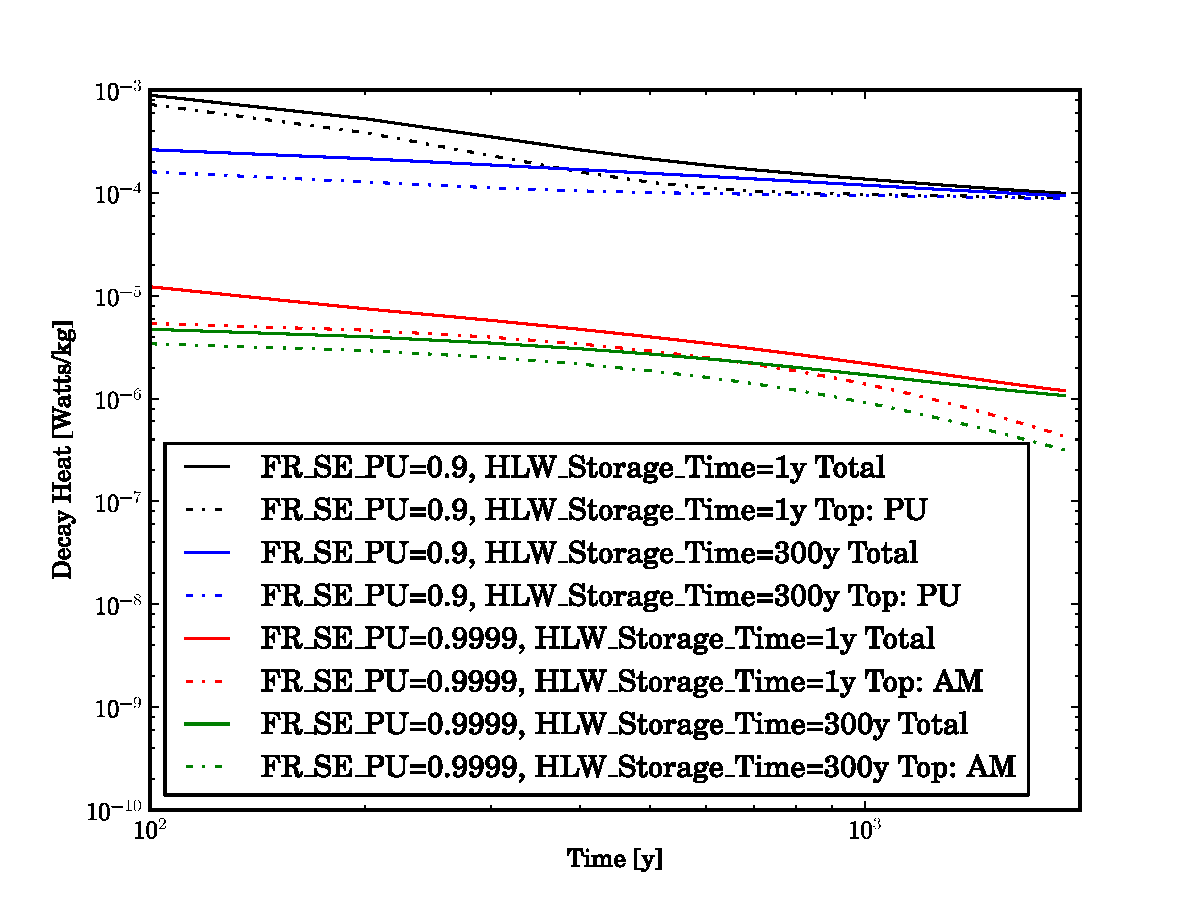
\includegraphics[scale=0.70]{figs/FR_SE_PU_and_HLW_Storage_Time_Decay_Heat.eps}
\caption{Total \& Top Contibutor Decay Heat [Watts/kg] of HLW for the parameter pair (\texttt{HLW\_Storage\_Time}, \texttt{FR\_SE\_PU}).}
\label{hlw_pu_decay_heat}
\end{center}
\end{figure}

Physically, the reason for this covariance is because the HLW storage 
time effectively shifts the opening time of the repository.
By having a long \texttt{HLW\_Storage\_Time}, the short- and medium-term 
repository tempurature limits may be avoided.
Figure \ref{hlw_pu_decay_heat} displays the decay heat for the HLW and for 
the top elemental contributor to the decay heat as a
function of time after emplacement in the repository.  The curves here 
represent the four corner cases of the input values.

The time shift effect may be observed by holding \texttt{FR\_SE\_PU} constant 
and comparing curves on Figure \ref{hlw_pu_decay_heat}
where \texttt{HLW\_Storage\_Time} is one year to the curves where the storage 
time is three hundred years.  Points on the 1 year curves have
roughly the same value as the 300 year HLW storage time curves, only 300 years 
farther in the future.  By shifting the 1 year data
three hundred years to the left, the two curves would nearly overlap.  The 
statistical analysis confirms the strong importance to repository capacity 
of a strategy of `waiting out' the decay of Pu-238 if Pu separation efficiencies 
are low, and its much weaker importance if efficiencies are high.

\section{Concluding Remarks \& Future Work}
\index{Concluding Remarks \& Future Work@\emph{Concluding Remarks \& Future Work}}
\label{cts_sec:conclusion}

The statistical techniques of contingency table and entropy analysis presented 
in this paper are widely-used tools for capturing the behavior of complex systems, 
particularly biological ones.  Here they have been applied to a simulator of the 
nuclear fuel cycle.  NFC outcomes, like those of any complex system, are shaped 
by intricate and highly nonlinear interactions between many inputs.

The strength of association between the inputs and the outcome studied here, the 
capacity of a Yucca Mountain-like repository, was quantified through uncertainty 
coefficients.  Three-dimensional uncertainties were augmented by a coefficient of 
variation to determine the system response inputs acting jointly.  The latter is 
especially important because alternative approaches, for instance linear sensitivity 
analyses, can only capture the response to departures from a reference state.  This 
reference state is defined by the values assumed by dozens or hundreds of system 
inputs, each of which may be varied by system or technology designers.  It was 
shown that the coefficient of variation could illuminate dependencies where changes 
in one input have a strong effect on the system response to another.  

This tool can aid system designers by helping them perceive which design variables 
matter.  The contingency tables represent a (coarsely-gridded) importance map for 
the inverse problem.  Conditioned on a specific system response, like repository 
capacity, the measure of the strength of response provided by the uncertainty coefficients 
can provide guidance to technologists optimizing design parameters in the face of uncertainty 
regarding the shape of the larger system.  Illuminating joint dependencies, coefficients of 
variation can guide iterative technology development by showing which design features must 
be considered together.

The approach described here can be generalized to include boolean as well as continuous inputs.  
For example, if the technology ultimately chosen for the permanent repository is unknown, 
a boolean flag can allow each stochastic realization to follow one of several options.  
The outcome, still repository capacity, would now be conditioned on this boolean input as well.  
It would illuminate system design parameters that will be important regardless of technology 
ultimately chosen, those that have strongly technology-dependent effects, and those that are 
unimportant to determining capacity regardless of technology.  In view of the uncertainties 
in the direction taken by nuclear energy in the future, coupled with the need to develop 
technologies now that can support or even enable these outcomes, this capability, if 
developed, could provide invaluable guidance.


\chapter{Multigroup Reactor Methodology}
\index{Multigroup Reactor Methodology@\emph{Multigroup Reactor Methodology}}

\section{Introduction}
\index{Introduction@\emph{Introduction}}
Previous studies have examined the use quickly executing, dominant physics codes for use in the
nuclear fuel cycle.  Unlike analytic techniques (such as neutron transport) which seek to completely 
solve fundemental physical systems, dominant physics codes parameterize the system and use interpolations
of results from stricter analytic methods to form a quick, run-time solution to the system at hand.

Dominant physics methods may be used for any fuel cycle component: enrichment, reactors, reprocesing, 
repositories, \emph{etc}.  However, their greatest advantage comes for such components whose analytic
techniques are computationally intensive.  Thus previous work has focused on reactors and repositories.

The dominant physics reactor methodologies to date have been one-energy group, fluenece-based parameterizations.
Neutron production \& destruction rates and transmutation matrices as a function of fluence 
(time-integrated flux) were recorded for each species initial present in the core.  A linear combination of 
the inital nuclides was then used to compute the multiplication factor, fuel burnup, and used fuel 
vector at discharge.

Unfortunately, because of the constant flux irradiation method used to generate the parameterizations, 
the above model was not sensitive to changes in the flux spectrum over the course of the burn.  The 
requirement of a static flux spectrum limits the type of reactors that may be studied using such a 
dominant physics methodology.  In seeking to expand the types of reactors model-able from the 
current fast reactors and light-water reactors, the flux spectrum must be folded back into the 
underlying parameterization.


\section{Multigroup Cross Section Generation}
\index{Multigroup Cross Section Generatrion@\emph{Multigroup Cross Section Generation}}
When seeking to parameterize nuclear power reactors as a function of initial conditions, 
the set of possible independent parameters quickly becomes large. In addition to geometric 
design considerations, the fuel characteristics of the reactor must also be accounted for.

In the one-energy-group reactor model (R1G), the initial loading was parameterized based
on neutron production rates, neutron destruction rates, and transmutation matrices per
nuclide \cite{Scopatz2009d}.  All of these metrics are a function of flunece.  (Under 
constant irradiation, fluence is a clear surrogate for time.)

A $G$-energy-group reactor model (RMG) seeks to re-parameterize the one-group formulation 
in terms of energy.  While the multi-group formulation will remain on a per nuclide basis, 
the neutron reaction rates do not have have a meaningful per unit energy expression that 
is independent of the flux.  Moreover changing reaction rates also invalidate the 
transmutation matrices.  

Therefore, the RMG, in a level of sophistication above the R1G, must be able to calculate
the multigroup flux spectrum.  To do so requires multigroup microscopic neutron cross-sections.  
Using the cross-sections as independent reactor parameters in a multigroup sense is 
effectively equivalent to removing the flux from the reaction rates in the one-group case.
This is seen in Equation \ref{reaction_rate_calc}
\begin{equation}
\label{reaction_rate_calc}
R = \sigma \cdot \phi \cdot 10^{-24}
\end{equation}
where $R$ [hz] is the reaction rate, $\sigma$ [barns] is the one-group cross section, and
$\phi$ [n/cm\superscript{2}/s] is the energy-integrated flux.

The remainder of this section is delineated into a discussion on notation, how initial 
reactor conditions are specified, the three methods that were used to compute the
cross sections, and the validation technique used.

\subsection{Notation}
\index{Notation@\emph{Notation}}
The group constants $\sigma_{itg}$ or $\sigma_{ipg}$ are themselves parameterized by nuclide, 
time or perturbation (see following section), and  incident neutron energy.  Nuclides are indexed by 
$i$, times are indexed by $t$, perturbations are indexed by $p$, and energy is indexed by $g$ with 
lower indices representing higher energy groups.

\begin{table}[htbp]
\begin{center}
\caption{Neutron Reaction Types}
\label{reaction_type_table}
\begin{tabular}{|l||c|c|}
\hline
\textbf{Tally}                              & \textbf{Symbol} & \textbf{MT} \\
\hline
Total                                       & $t$             & 1  \\
Scattering                                  & $s$             & 2 + 4 \\
Elastic Scattering                          & $e$             & 2 \\
Inelastic Scattering                        & $i$             & 4 = sum(51, 91) \\
$n$\superscript{th}-state Inelastic Scatter & $i\{n\}$        & 50 + $n$ \\
(n, 2n)                                     & $2n$            & 16 \\
(n, 3n)                                     & $3n$            & 17 \\
Fission                                     & $f$             & 18 = 19 + 20 + 21 +38 \\
First-chance Fission                        & $f19$           & 19 \\
Second-chance Fission                       & $f20$           & 20 \\
Third-chance Fission                        & $f21$           & 21 \\
Fourth-chance Fission                       & $f38$           & 38 \\
Absorption                                  & $a$             & 27 = 18 + sum(102, 107) \\
Neutron Capture                             & $\gamma$        & 102 \\
Proton                                      & $p$             & 103 \\
Deuterium                                   & $d$             & 104 \\
Tritium                                     & \nuc{H}{3}      & 105 \\
Helium-3                                    & \nuc{He}{3}     & 106 \\
Alpha                                       & $\alpha$        & 107 \\
Metastable Neutron Capture                  & $\gamma*$       & $\dagger$ \\
Metastable (n, 2n*)                         & $2n*$           & $\dagger$ \\
\hline
\end{tabular}
\end{center}
\end{table}


To fully describe a reactor, several neutron reaction types are required.  The type 
also augments the group constant notation by being a comma-separated preposition to 
the index.  For example, the total cross section would be represented by the symbol 
$\sigma_{t,itg}$. Table \ref{reaction_type_table} displays the reactions used in this 
study, their symbolic abbreviations, and the corresponding MT number coming from ENDF 
specification \cite{MFMT}.  Entries whose MT number is given as a $\dagger$ indicates 
that the generation of these tallies was performed in a special way (see below).
Additionally, the group-to-group scattering cross section is denoted by the symbol
$\sigma_{s,itgh}$ where $g$ denotes the incident neutron energy (as before) and $h$
gives the exiting neutron energy.

\subsection{Parameterization of Initial Conditions}
\index{Parameterization of Initial Conditions@\emph{Parameterization of Initial Conditions}}
The multigroup reactor model requires a library of pre-computed group constants which it uses
to calculate run-time cross section values for the core.  This library must therefore satisfy 
two conditions.  The first is that it contain group constant information for all independent, 
mutable parameters of interest.  The second is that the parameter values must span 
their corresponding range of interest.  

Changes in the initial parameter conditions would then elicit changes in the cross section 
values. Differences in the group constants would thus be picked up by the RMG.  For example, 
take the case of neutron self-shielding in a material with a strong resonance absorption peak.  
As the number density of the absorber increases, the group constant in the spectrum around 
the peak may plummet because the flux bottoms out.  In a relatively dilute medium, the group 
constant and the flux would increase because fewer neutrons (in an absolute sense) are destroyed 
in this regime.  That the  cross section library captures such effects is the primary advantage 
of a multigroup model over the traditional one-group method.

\begin{table}[htbp]
\begin{center}
\caption{CHAR Parameters that Define a Perturbation}
\label{char_perturbable_variables}
\begin{tabular}{|l|c|c|}
\hline
\textbf{Parameter}            & \textbf{Symbol}      & \textbf{Units} \\
\hline
Fuel Density                  & $\rho_{\mbox{fuel}}$ & g/cm\superscript{3}  \\
Cladding Density              & $\rho_{\mbox{clad}}$ & g/cm\superscript{3}  \\
Coolant Density               & $\rho_{\mbox{cool}}$ & g/cm\superscript{3}  \\
Fuel Cell Radius              & $r_{\mbox{fuel}}$    & cm \\
Void Cell Radius              & $r_{\mbox{void}}$    & cm \\
Cladding Cell Radius          & $r_{\mbox{clad}}$    & cm \\
Unit Cell Pitch               & $\ell$               & cm \\
Number of Burn Regions        & $b_r$                &  \\
Fuel Specific Power           & $p_s$                & MW/kgIHM \\
Initial Nuclide Mass Fraction & $T_{i0}$             & kg\subscript{i}/kgIHM \\
Burn Times                    & $s$                  & days \\
\hline
\end{tabular}
\end{center}
\end{table}

The code which produces the cross section library is known as CHAR (CITEME).  Char currently
has the ability to adjust a reactor template based on many initial parameters.  These fall
conceptually into three categories: geometric properties, material properties, and time.
Table \ref{char_perturbable_variables} lists the parameters that define a \emph{perturbation}
in char.

\begin{table}[htbp]
\begin{center}
\caption{CHAR Outer Product Perturbations}
\label{char_param_outer_product}
\begin{tabular}{|ccccccccccc|}
\hline
\textbf{$\rho_{\mbox{fuel}}$} & \textbf{$\rho_{\mbox{clad}}$} & \textbf{$\rho_{\mbox{cool}}$} & \textbf{$r_{\mbox{fuel}}$} & \textbf{$r_{\mbox{void}}$} & \textbf{$r_{\mbox{clad}}$} & \textbf{$\ell$} & \textbf{$b_r$} & \textbf{$p_s$} & \textbf{$T_{\mbox{\nuc{U}{235}0}}$} & \textbf{$s$} \\
\hline
10.165 & 5.87 & 0.73 & 0.41 & 0.4185 & 0.475 & 1.3127 & 10 & 0.04 & 0.03 & 0    \\ 
10.165 & 5.87 & 0.73 & 0.41 & 0.4185 & 0.475 & 1.3127 & 10 & 0.04 & 0.03 & 2100 \\ 
10.165 & 5.87 & 0.73 & 0.41 & 0.4185 & 0.475 & 1.3127 & 10 & 0.04 & 0.03 & 4200 \\ 
10.165 & 5.87 & 0.73 & 0.41 & 0.4185 & 0.475 & 1.3127 & 10 & 0.04 & 0.05 & 0    \\ 
10.165 & 5.87 & 0.73 & 0.41 & 0.4185 & 0.475 & 1.3127 & 10 & 0.04 & 0.05 & 2100 \\ 
10.165 & 5.87 & 0.73 & 0.41 & 0.4185 & 0.475 & 1.3127 & 10 & 0.04 & 0.05 & 4200 \\ 
11.235 & 5.87 & 0.73 & 0.41 & 0.4185 & 0.475 & 1.3127 & 10 & 0.04 & 0.03 & 0    \\ 
11.235 & 5.87 & 0.73 & 0.41 & 0.4185 & 0.475 & 1.3127 & 10 & 0.04 & 0.03 & 2100 \\ 
11.235 & 5.87 & 0.73 & 0.41 & 0.4185 & 0.475 & 1.3127 & 10 & 0.04 & 0.03 & 4200 \\ 
11.235 & 5.87 & 0.73 & 0.41 & 0.4185 & 0.475 & 1.3127 & 10 & 0.04 & 0.05 & 0    \\ 
11.235 & 5.87 & 0.73 & 0.41 & 0.4185 & 0.475 & 1.3127 & 10 & 0.04 & 0.05 & 2100 \\ 
11.235 & 5.87 & 0.73 & 0.41 & 0.4185 & 0.475 & 1.3127 & 10 & 0.04 & 0.05 & 4200 \\ 
\hline
\end{tabular}
\end{center}
\end{table}

Every parameter is specified with one or more values.  The outer product of all parameter
values defines the set of perturbations for which the group constants are calculated.
The total number of perturbations, $n_p$, is therefore given by the product of 
the lengths of the parameter arrays.  \emph{In concreto}, Table \ref{char_param_outer_product} 
displays the perturbations when the fuel density has two values, the initial \nuc{U}{235} mass 
fraction also takes two values, the group constants are calculated at three burn steps, and all 
other parameters are single valued

While Table \ref{char_param_outer_product} represents a simple set of reactors, this formulation 
allows for the easy expansion and extension of input parameters, and thus new perturbations. 
Including additional values for any parameter would extend the number of rows in the table.  
Including other parameters, such as initial \nuc{U}{236} concentration, would expand the number of
columns in the perturbation table, effectively increasing the dimensionality parameterized.
A particularly aggressive strategy would be to include the mass fractions of all actinides initially
present in the core.  In a recycle scenario, this would increase the number of parameters by 
approximately an order of magnitude.  

For the remainder of the this study the perturbations presented in Table \ref{char_param_outer_product}
were sufficient to demonstrate the validity of the multigroup method.

\subsection{Cross Section Generation: Serpent}
\index{Cross Section Generation: Serpent@\emph{Cross Section Generation: Serpent}}
\label{mg:xs_gen_serpent}
Of the over 3000 nuclides, continuous cross section information is available for only 
approximately 400 major species.  Moreover, not all reactions are tallied 
for these nuclides.  However, where fundamental cross section data exists for a nuclide
and a reaction, it is preferable to use this high-fidelity information to compute group
constants over other methods discussed below.

$G$-group cross sections are assembled for each perturbation using the Monte Carlo neutron
transport code Serpent \cite{Lepp2011}.  Char fills a templated Serpent input deck with the
perturbation values and then executes the transport code.  The templates use a combination 
of detectors in the fuel, cladding, and coolant regions as well as the universe metrics that 
Serpent outputs to determine the group constants.

In almost every case, the detectors specified with the appropriate MT number suffice.  
However, some tallies (and some reaction-like parameters) are not given by detectors
but are still computable via Serpent.

Foremost of the non-standard calculations is the group-to-group scattering cross section
$\sigma_{s,ipgh}$.  Among the region-based output of Serpent are both a group transfer
probability matrix $P_{gh}$ as well as the group-to-group scattering cross section
as calculated via the constraints in equations \ref{gtg_constraint} \& \ref{gtg_calc}.
\begin{equation}
\label{gtg_constraint}
\sum_h^G P_{gh} = 1
\end{equation}
\begin{equation}
\label{gtg_calc}
\sigma_{s,gh} = P_{gh} \cdot \sigma_{s,g}
\end{equation}
However, the group transfer probability, and thus the group-to-group scattering cross sections
are functions of the entire region and not individual species within that region.  

Unfortunately, the RMG itself requires that the group-to-group scattering cross sections be provided 
per nuclide. To this end, the authors modified the source code of Serpent to include an optional 
additional mode where $P_{gh}$ is calculated for only a specific sub-material in a region.    
Using this mode with a single nuclide material and the detector calculated
scattering cross section $\sigma_{s,ipg}$, the group-to-group scattering cross section was computed 
for a single species via equation \ref{gtg_calc}.

The next supplemental calculation that char performs comes more from a deficiency in the 
ENDF specification than from Serpent.  Reactions which leave the final nucleus in an energy
state above ground do not receive separate MT numbers.  Moreover, some of these excited states
are metastable and may persist long enough in the core to have a significant interaction 
probability of their own.  Additionally, certain metastable nuclides, such as \nuc{Am}{242}\superscript{*},
persist for long enough that they have noticeable impacts on the fuel cycle, specifically with regards to 
the repository.  That metastable nuclides have their own continuous energy cross section libraries
but can not be generated by the reactions in these libraries is a perennial issue.

Here the metastable issue is circumvented by using the 64-group cross section library from CINDER that is 
included with MCNPX versions 2.6+ \cite{Pelowitz2008}.  The Cinder cross sections include metastable
interactions where available.  Serpent is then used to compute a `high-resolution' 
flux spectrum which matches the group structure of the Cinder data for each perturbation.  
Collapsing the metastable and ground cross sections to $G$-groups and dividing the former by 
the later gives a metastable-to-ground ratio $r_{\mbox{meta}}$.  This ratio may then be used along with 
the Serpent tally to calculate the group constants desired, as seen in equations \ref{msground} \& 
\ref{msex}.
\begin{equation}
\label{msground}
\sigma_{\gamma,ipg} = \frac{\sigma_{\gamma_{\mbox{tot}},ipg}}{1 + r_{\mbox{meta}}}
\end{equation}
\begin{equation}
\label{msex}
\sigma_{\gamma*,ipg} = r_{\mbox{meta}} \cdot \sigma_{\gamma,ipg}
\end{equation}
In equation \ref{msground}, the $\sigma_{\gamma_{\mbox{tot}},ipg}$ represents the total neutron
capture cross section as provided by the Serpent via MT 102.  However, Cinder 
lists the ground and metastable states separately.  For most nuclides that do not have a metastable state, the 
ground state interaction is the total (\emph{i.e.} $\sigma_{\gamma,ipg} = \sigma_{\gamma_{\mbox{tot}},ipg}$).
The RMG expects the interaction tallies to be split out, as in Cinder.  Analogous equations are 
derivable for the (n, 2n*) interaction.

Furthermore, the average number of neutrons produced per fission event $\bar{\nu}$ is also 
calculated in special way via Serpent.  The pseudo-tally number $-7$ yields $\bar{\nu}\sigma_{f,ipg}$.
Using the fission group constant calculated from serpent in the usual way, an expression for $\bar{\nu}$
is trivially obtained (equation \ref{mg_nubar}).
\begin{equation}
\label{mg_nubar}
\bar{\nu}_{ipg} = \frac{\bar{\nu}\sigma_{f,ipg}}{\sigma_{f,ipg}}
\end{equation}

The final pseudo-tally that is calculated via serpent is the fission neutron energy spectrum, $\chi(E)$.
The continuous energy cross section data libraries do not contain information on $\chi(E)$.  However, 
Serpent outputs per group values for this parameter for different regions.  While this does not 
capture per nuclide effects, $\chi(E)$ varies only slightly among different species.  
Moreover, since a Serpent run is performed for each perturbation, changes to 
the initial conditions are still encapsulated.  Thus the induced error on the RMG is very low.


\subsection{Cross Section Generation: Physical Models \& CINDER}
\index{Cross Section Generation: Physical Models@\emph{Cross Section Generation: Physical Models}}
\label{mg:xs_gen_physics}
As mentioned in \S \ref{mg:xs_gen_serpent}, continuous energy cross section data is available for only 
a small fraction of the nuclides, though arguably the most important ones.  However, some species 
may have significant fuel cycle importance and yet do not have the highest-fidelity data available.

In this case, Char and the RMG `fall-back' to using a combination of Cinder data and fundamental 
physical models to estimate the group constants. The first stage in this calculation, as with the 
metastable-to-ground ratio, is to use Serpent to compute a 64-group high-fidelity flux $\phi_n$
which matches the structure used in the Cinder library.  If Cinder data exists for a nuclide for 
a reaction, a simple collapse down to $G$-groups is performed.  For other reactions physical
models are used.  In all cases if Cinder data and physical models are not available, then group
constants of zero are assumed.  Note that group constants tabulated in this way, while dependent 
on changes in the spectrum, are independent of effects such as self-shielding.
The remainder of this section discusses the reactions individually.

First, Cinder includes cross section information for fission reactions.  If a nuclide does not 
contain fission cross section information it is a safe assumption that either the species 
is not fissionable or is an actinide of such high order that it exists in a reactor in vanishingly 
small quantities.  If $n$ indexes $N=64$ groups from Cinder and $E$ [MeV] denotes the energy boundaries, 
the $G$-group collapsed fission cross section may be computed as in equation \ref{fiss_group_collapse}.
\begin{equation}
\label{n_lower}
n_l = \min(n|E_g<E_n)
\end{equation}
\begin{equation}
\label{n_upper}
n_u = \max(n|E_n<E_{g+1}) - 1
\end{equation}
\begin{equation}
\label{f_lower}
f_l = \frac{E_{n_l} - E_g}{E_{n_l} - E_{n_l-1}}
\end{equation}
\begin{equation}    
\label{f_upper}
f_u = \frac{E_{g+1} - E_{n_u}}{E_{n_u+1} - E_{n_u}}
\end{equation}
\begin{equation}
\label{fiss_group_collapse}
\sigma_{f,ipg} = \frac{f_l\sigma_{f,ipn_l-1}\phi_{n_l-1} + \sum_{n=n_l}^{n_u} \sigma_{f,ipn}\phi_n + f_l\sigma_{f,ipn_u+1}\phi_{n_u+1}}{f_l\phi_{n_l-1} + \sum_{n=n_l}^{n_u} \phi_n  + f_u\phi_{n_u+1}}
\end{equation}
Equations \ref{n_lower}-\ref{f_upper} define lower and upper indices and linear energy fractions
which aid in calculating group constants in which the boundaries only partially overlap.

Cinder does not include $\bar{\nu}$ data and so for nuclides where the fission cross-section is 
non-zero, a constant value of 2.5 was assumed. Cinder also does not include fission neutron 
spectrum information.  Where fission is possible, the physical model seen in equation \ref{chi_model}
was discretized to $G$-groups.
\begin{equation}
\label{chi_model}
\chi(E) = 0.453 \cdot e^{-1.036E} \cdot \sinh\left(\sqrt{2.29E}\right)
\end{equation}
This spectrum comes from \nuc{U}{235}, but may be used for other nuclides as well \cite{Lamarsh2002}.

Non-fission absorption reaction cross sections ($\gamma$, 2n, 3n, $p$, $d$, \nuc{H}{3}, \nuc{He}{3}, 
$\alpha$, $\gamma*$, 2n*) are computed similarly to the fission group constant.  If a reaction 
type is available in Cinder, a group collapse on the 64-group data is performed.  If the reaction 
type is not present for a nuclide, the interaction is assumed to be impossible and zero values
are returned.

The absorption cross section $\sigma_{a,ipg}$ is simply the sum of its constituent elements, as 
computed above.  Set $r_x$ as a non-fission absorption reaction type, then
\begin{equation}
\label{sig_a_model}
\sigma_{a,ipg} = \sigma_{f,ipg} + \sum_{r_x} \sigma_{r_x,ipg}
\end{equation}
Cinder includes several reactions that are not tracked by the RMG or Char, such as (n, 4n). 
However, these interactions are included in the absorption reaction estimate here.  

Considerably more complicated is the physical model of the scattering cross section.  Unfortunately, 
Cinder provides no pretabulated 64-group data to collapse.  Moreover, the group-to-group scattering
cross section $\sigma_{s,ipgh}$ is desired, adding an additional dimension to compute.
Furthermore, because scattering reactions are mainly about energy transfer between the neutron and 
nuclide, the material temperature $T$ [K] is also important.

Equation \ref{scat_ce} represents a continuous energy model of the scattering cross section for a free gas
\cite{Yamamoto2006, Mattes2005}.
\begin{equation}
\label{scat_ce}
\sigma_s(E) = 4 \pi b^2 \cdot \left(1 - \frac{2E}{931.46 \cdot m_n}\right) \cdot
              \left(1 + \frac{m_n}{M_A} \frac{kT}{E} \cdot e^{-\frac{M_A}{m_n}\frac{E}{kT}}\right) 
              \cdot \left(1 - \mbox{Exp}\left[-\sqrt{\frac{0.1}{E}}\right]\right)
\end{equation}
where $b$ [cm] is the bound scattering length of the target nucleus, $E$ [MeV] is the incident
neutron energy, $m_n$ is mass of the neutron, $M_A$ is the mass of the target nucleus, and
$k$ [MeV/K] is Boltzmann's constant.

Term by term, $4 \pi b^2$ represents a base estimate of the scattering cross section.  
The $\left(1 - \frac{2E}{931.46 \cdot m_n}\right)$ term is a relativistic correction
factor for $b$.  The remaining two terms are an adjusted, neutron-exiting-energy-integrated 
representation of the scattering kernel $S(\alpha, \beta)$ for a free gas.

The bound scattering length for a nuclide is computed via coherent and incoherent components
(equation \ref{scat_len}).
\begin{equation}
\label{scat_len}
b = \sqrt{\left| b_{\mbox{coh}} \right|^2 + \left| b_{\mbox{inc}} \right|^2}
\end{equation}
Values for the scattering lengths were obtained from \cite{Sears1992}.  For nuclides
that do not appear in this tabulation, a $b$-value for a nuclide of the same element was
used as a surrogate.  If the entire element was absent from the tabulation, then the 
scattering length of the next lowest Z-numbered nuclide was substituted instead.

The group-to-group scattering cross section may thus be calculated as in equation \ref{scat_collapse}.
\begin{equation}
\label{scat_collapse}
\sigma_{s,gh} = \frac{\int_{E_g}^{E_{g+1}} \int_{E_h}^{E_{h+1}} \sigma_s(E) P(E \to E^\prime) \phi_g(E) dE^\prime dE}
                     {\int_{E_g}^{E_{g+1}} \phi_g(E) dE}
\end{equation}
with $E^\prime$ as the exiting neutron energy and $P(E \to E^\prime)$ being the differential probability of 
scattering from one energy to another.  This probability is computed via equation \ref{P_E_to_E_prime}
\begin{equation}
\label{P_E_to_E_prime}
P(E \to E^\prime) = \frac{1}{E + kT - \left(\frac{M_A - m_n}{M_A + m_n}\right)^2 E}
\end{equation}
Note that equation \ref{P_E_to_E_prime} is only valid on the range 
\begin{equation}
\label{P_E_to_E_prime_range}
\left(\frac{M_A - m_n}{M_A + m_n}\right)^2 \cdot E \le E^\prime \le E + kT
\end{equation}
For all values of $E^\prime$ outside of this range, $P(E \to E^\prime) = 0$.

Subjecting the numerically computed the double integral in equation \ref{scat_collapse} 
to the incident scattering constraint yields the appropriate group constant (equation \ref{scat_constraint}).
\begin{equation}
\label{scat_constraint}
\sigma_{s,g} = \sum_h^G \sigma_{s,gh}
\end{equation}

Finally, the total cross section may be expressed as the sum between the absorption and scattering
cross sections, as computed in the models above.
\begin{equation}
\label{tot_xs_model}
\sigma_{t,g} = \sigma_{s,g} + \sigma_{a,g}
\end{equation}

\subsection{Cross Section Generation: Interpolation}
\index{Cross Section Generation: Interpolation@\emph{Cross Section Generation: Interpolation}}
\label{mg:xs_gen_interpolation}
The last class of nuclides are those for which there is no continuous energy cross section data 
available and which do not have enough of a fuel cycle impact that warrants computing group constants 
via physical models.  Due to the unimportance of these species, only the roughest of estimates
of their cross sections are needed.  Moreover, such estimation may be done at RMG run-time rather 
than during library generation.

The Korea Atomic Energy Research Institute (KAERI) provides simple cross section information
for almost 3000 nuclides at a variety of energies \cite{KAER2000}.  Specifically, data for
thermal (2.53E-08 [MeV]) and fission spectrum average (taken as 1.0 [MeV]) were used as representative
thermal and fast cross sections.  Ignoring all other effects (particularly epithermal resonances), 
group constants were computed by linearly interpolating these two cross sections.  Call 
$\sigma_{r_x}^t$ and $\sigma_{r_x}^f$ the thermal and fast cross sections respectively.  The group
constants for a reaction $r_x$ were estimated using equation \ref{group_const_est}.
\begin{equation}
\label{group_const_est}
\sigma_{r_x,g} = \frac{\sigma_{r_x}^f - \sigma_{r_x}^t}{1 - \mbox{2.53E-08}} \cdot (E_g - \mbox{2.53E-08}) + \sigma_{r_x}^t
\end{equation}
In the case where even this method fails (negative cross sections computed or data not available), 
a zero values is finally assumed for this group constant.

\subsection{Cross Section Validation}
\index{Cross Section Validation@\emph{Cross Section Validation}}
\label{mg:xs_validation}
Due to the quantity of cross section data produced through the three above methods, the 
impossibility of comprehensively visually inspecting it all for `goodness', and the errors 
prone to human inspection, an automatic validation procedure known as \emph{unit testing}
was employed.  Here, the units are interpreted as the group constants.   A suite of tests 
executed against these units ensures that the cross sections remain physically valid 
individually as well as in relation to each other. What follows are the definitions of the 
physical tests which make up the suite.  All cross sections present in the library were tested 
in this manner.

The most basic test is to verify that all group constants are real and non-negative valued 
(infinite and not-a-number values are not allowed).  
\begin{equation}
\label{nn_ut}
0 \le \sigma_{r_x,ipg} < \infty
\end{equation}
While this may seem to be a trivial 
condition, if such values are allowed to pass through, a single bad group-constant may 
propagate to all portions of an RMG calculation.

No less important, is the constraint that all group constants are less than or equal to 
the total cross section.
\begin{equation}
\label{tot_xs_ut}
\sigma_{r_x,ipg} \le \sigma_{t,ipg}
\end{equation}
Moreover, if a nuclide is fissionable, the following conditions apply.
\begin{equation}
\label{nu_fiss_ut}
1 \le \bar{\nu}_{ipg} \le 5.5
\end{equation}
\begin{equation}
\label{chi_fiss_ut}
\sum_g^G \chi_{ipg} = 1
\end{equation}
If the nuclide is not fissionable, the following conditions are used instead.
\begin{equation}
\label{not_fiss_ut}
\sigma_{f,ipg} = \bar{\nu}_{ipg} = \chi_{ipg} = 0
\end{equation}
The relation between scattering group constants is defined as follows, to 
within machine precision.
\begin{equation}
\label{scat_xs_ut}
\sigma_{s,ipg} = \sum_h^G \sigma_{s,ipgh}
\end{equation}
Lastly, it is required that the constituent absorption tallies sum 
to less than or equal to the absorption cross section.
\begin{equation}
\label{scat_xs_ut}
\sum_{r_x} \sigma_{r_x,ipg} \le \sigma_{a,ipg}
\end{equation}
Further conditions could be added to the suite, such as ensuring that the sum of 
all non-total group constants is less than equal to $\sigma_{t,ipg}$.  However, 
such summation tests are typically indicative of a more primitive error in the 
group constants.  These basic errors are sufficiently captured by the tests above, 
without adding extraneous noise to the failure analysis.  The simple test suite developed
here has proven invaluable towards the RMG benchmarking efforts.




\section{Multigroup Reactor Model}
\index{Multigroup Reactor Model@\emph{Multigroup Reactor Model}}
\label{mg_sec:rmg_model}
The multigroup reactor model uses the group constant library developed in the previous 
section to compute criticality and burnup metrics for a nuclear power reactor (NPR).
The RMG is specified by a several parameters, including all those present in Table
\ref{char_perturbable_variables}.

However, the advantage of the RMG method here is that the values of the reactor parameters
need not exactly match any of the perturbations (Table \ref{char_param_outer_product}) in the 
cross section library.  Other methods are often invalidated when the conditions under which 
the group constants were computed are altered.  However, by including a robust set of values
in the perturbation table, the RMG execution remains meaningful.

% Define block styles
\tikzstyle{decision} = [diamond, very thick, draw, fill=red!75, text width=4.5em, text badly centered, node distance=3cm, inner sep=0pt]
\tikzstyle{block} = [rectangle, draw,  very thick, fill=white!20, text width=5em, text centered, rounded corners, minimum height=2em]
\tikzstyle{line} = [draw, very thick, color=black!100, -latex']
\tikzstyle{cloud} = [draw, ellipse,fill=red!20, node distance=3cm, minimum height=2em]

\begin{figure}
\caption{Multigroup Reactor Model Method Diagram}
\label{rmg_method_diagram}
\begin{tikzpicture}[node distance = 5cm, auto]
    % Place nodes
	\node [block, text width=12em, sharp corners] (known) {\underline{Known}: from library,\\ 
		$\bullet$ $\sigma_{r_x,ipg}$ \, $\bullet$ $\bar{\nu}_{ipg}$\\
		$\bullet$ $\sigma_{s,ipgh}$  \, $\bullet$ $\chi_{ipg}$};
	\node [block, fill=green!20, right of=known] (given) {\underline{Given}:\\
		$t=0$};
	\node [block, text width=20em, fill=blue!20, below of=given, node distance=2.5cm] (interpolate) {\underline{Interpolate}:
		find $\left\{ m | \Phi_m \leq \Phi_n \leq \Phi_{m+1} \right\}$\\
		$f(\Phi_n,i) = \frac{f(\Phi_{m+1}) - f(\Phi_m)}{\Phi_{m+1} - \Phi_m} (\Phi_n - \Phi_m) + f(\Phi_m)$\\
		for $f$ in $\left[w^0, \sigma^0, \Delta\sigma \right]$,\\ 
		using $\Delta w(\Phi_n, i)=w^0(\Phi_n,i)-w(\Phi_n,i)$};
	\node [block, below of=interpolate, fill=yellow!40, text width=20em, node distance=2.5cm] (eigen) 
		{\underline{Calculate}:\\
		$\bullet$ $A(\Phi_n)=A^0(\Phi_n)+\Delta A(\Phi_n, \Delta w(\Phi_n, i))$\\
		$\bullet$ $F(\Phi_n)=F^0(\Phi_n)+\Delta F(\Phi_n, \Delta w(\Phi_n, i))$\\
		$\bullet$ $\left( A(\Phi_n) - \frac{1}{k}F(\Phi_n) \right)\phi(\Phi_n)=0$};
	\node [block, left of=eigen, node distance=5.5cm, fill=purple!20] (store1){\underline{Store}:\\
		$\phi_g(\Phi_n)$\\
		$k(\Phi_n)$};
	\node [block, text width=14em, fill=blue!20, below of=store1, node distance=2.5cm] (set) {\underline{Set}:\\
		$\Delta t=t_{n+1}-t_n$\\
		$\Phi_{n+1} = \Phi_n + \Delta t \sum_{g=1}^G \phi_g(\Phi_n)$};
	\node [block, text width=20em, below of=eigen, fill=yellow!40, node distance=5cm] (transmute){\underline{Transmute}:\\
		$w(\Phi_{n+1},i)=e^{M(\Phi_n)\Delta t}w(\Phi_n,i)$\\
		\underline{Calculate}: $\mbox{BU}(\Phi_{n+1})$};
	\node [block, above of=transmute, node distance=2.5cm, fill=purple!20] (store2){\underline{Store}:\\
		$w(\Phi_{n+1},i)$\\
		$\mbox{BU}(\Phi_{n+1})$};
	\node [decision, right of=store2, text width=5.5em, node distance=4.5cm] (morestep) {\underline{More steps?}\\
		$\Phi_n\to \Phi_{n+1}$\\
		$n\to n+1$};
	\node [block, below of=morestep, text width=10em, sharp corners] (continue) 
		{\underline{Continue}: Keep going with prior methodology.}; 

	% Draw edges
	\path [line] (known) -- (given);
	\path [line] (given) -- (interpolate);
	\path [line] (interpolate) -- (eigen);
	\path [line] (eigen) -- (store1);
	\path [line] (store1) -- (set); 
	\path [line] (set) |- (transmute);
	\path [line] (transmute) -- (store2);
	\path [line] (store2) -- (morestep);
	\path [line] (morestep) |- node [pos=0.2] {yes} (interpolate);
	\path [line] (morestep) -- node [pos=0.5] {no}  (continue);
\end{tikzpicture}
\end{figure}


A flow sheet for the RMG methodology is presented in Figure \ref{rmg_method_diagram}.  As is
seen, the reactor model contains three main calculation stages for each burn time step.
First there is a nearest neighbor \& interpolation calculation for determining the group
constants for this time step.  Following this is flux-criticality calculation.  Lastly, the reactor
has a burnup-transmutation computation before continuing to the next time step.  The algorithms
implemented are discussed in \S \ref{mg_sec:nn_xs}-\ref{mg_sec:trans_calc}.


\subsection{Nearest Neighbor Cross Section Calculation}
\index{Nearest Neighbor Cross Section Calculation@\emph{Nearest Neighbor Cross Section Calculation}}
\label{mg_sec:nn_xs}
The process of converting from the perturbation-based cross section library $\sigma_{r_x,ipg}$ to 
group constants as a function of burn time in the RMG $\sigma_{r_x,itg}$ involves a nearest 
neighbor calculation as well as a multi-dimensional linear interpolation.

Call $a$ a perturbable reactor parameter, such as fuel density or burn time (\emph{i.e.} the 
columns in Table \ref{char_perturbable_variables}).   With $p$ as the perturbation index 
such that $1 \le p \le n_p$ (\emph{i.e.} the row number of Table \ref{char_param_outer_product}), 
then $a_p$ denotes the value of this reactor parameter for this perturbation.  Furthermore, call
$a_r$ the value of this parameter on the reactor model itself.

In order to perform the correct interpolation, the two perturbations that are closest to the current
state of the reactor, $a_1^*$ \& $a_2^*$, must be found.  Here the $a_p^*$ notation indicates that 
the indices have been sorted in order of increasing distance.  

However, the space that the reactor parameters live in is at least 10-dimensional.  Moreover, 
the scale for these parameters may vary greatly from one $a$ to the next.  Therefore, a realistic
nearness metric must normalize the values for these parameters individually before calculating a
global distance.  Equation \ref{nn_distance} calculates $d_p$, the distance of the $p$\superscript{th} 
perturbation from the state of reactor.
\begin{equation}
\label{nn_distance}
d_p = \sqrt{\sum_a \left(\frac{a_r - a_p}{a_{n_p}}\right)^2}
\end{equation}
Thus $p^*$ and $a_p^*$ are defined via the sequence $p^* = \left\{p | d_p \le d_{p+1}\right\}$.

Since $a_1^*$ and $a_2^*$ represent the value of a parameter at the two closest pertubations to the
current state of the reactor, a unitless multidimentional linear interpolation factor $x_f$ may be defined.
\begin{equation}
\label{x_factor}
x_f = \sum_a \left(\frac{a_r - a_1^*}{a_2^* - a_1^*}\right)
\end{equation}
This is then used to generate group constants for all reactions at all times from perturbation information
available in the cross section library. 
\begin{equation}
\label{sig_multi_interp}
\sigma_{r_x,itg} = (\sigma_{r_x,ip_2^*g} - \sigma_{r_x,ip_1^*g}) \cdot x_f  + \sigma_{r_x,ip_1^*g}
\end{equation}
Note, that $x_f$ is invalidated whenever the state of the reactor changes.  Since burnup time is one of 
the parameters, $x_f$ must be recalculated every time step but is otherwise constant for all nuclides
for all reactions.


\subsection{Criticality Calculation}
\index{Criticality Calculation@\emph{Criticality Calculation}}
\label{mg_sec:crit_calc}
Now that group constants have been built for the reactor specified, the next phase of the reactor 
calculation is to estimate the neutron flux spectrum and the multiplication factor given the current 
material stream of the core. (Naturally, the initial heavy metal stream must be provided.)

The flux spectrum is computed through an interative matrix method.  Call $N_{q,it}$ [atoms/cm\superscript{3}] 
the number density for the $i$\superscript{th} nuclide at time $t$ in the $q$\superscript{th} region 
(fuel, cladding, coolant).  The macroscopic cross section of a region is therefore given by equation 
\ref{region_xs}.
\begin{equation}
\label{region_xs}
\Sigma_{r_x,q,tg} = \sum_i^I N_{q,it} \cdot \sigma_{r_x,itg}
\end{equation}
Since the fuel and coolant are the only two regions with significant neutronic characterisics, 
homogenized full-core cross sections are given by the reduction in equation \ref{region_collapse}
\begin{equation}
\label{region_collapse}
\Sigma_{r_x,tg} = \frac{V_{\mbox{fuel}}\Sigma_{r_x,\mbox{fuel},tg} + \zeta_{tg}V_{\mbox{cool}}\Sigma_{r_x,\mbox{cool},tg}}
                       {V_{\mbox{fuel}} + \zeta_{tg}V_{\mbox{cool}}}
\end{equation}
Here, $\zeta_{tg}$ is the thermal disadvantage factor per group.  This is computed via the macroscropic 
cross sections and the lattice functions found in \cite{Lamarsh2002}.

The absorption or $A$-matrix is defined as 
\begin{equation}
\label{A_matrix}
A_{tgh} = I_G \times \Sigma_{t,tg} - \Sigma_{s,tgh}
\end{equation}
where $I_G$ is the $G \times G$ identity matrix. The fission source or $F$-matrix is defined by
\begin{equation}
\label{F_matrix}
F_{tgh} = \chi_{\mbox{fuel},tg} \times \bar{\nu} \Sigma_{f,\mbox{fuel},tg}
\end{equation}
The multigroup flux spectrum is then calculated via the linear relation in equation \ref{A_eq_F}.
\begin{equation}
\label{A_eq_F}
A_{tgh} \cdot \phi_{tg} = \frac{1}{k} F_{tgh} \cdot \phi_{tg}
\end{equation}
To solve this equation in an efficient iteraive fashion, note that the expression 
$\frac{1}{k}A^{-1}F$ is a single matrix.  Using the superscript $m$ to indicate the loop
index, equations \ref{next_flux} \& \ref{next_k} may be successively applied 
until convergence.
\begin{equation}
\label{next_flux}
\phi_{tg}^{m+1} = \frac{1}{k^m} A_{tgh}^{-1} F_{tgh} \cdot \phi_{tg}^{m+1}
\end{equation}
\begin{equation}
\label{next_k}
k^{m+1} = k^m  \frac{\sum_g^G \bar{\nu} \Sigma_{f,\mbox{fuel},tg} \phi_{tg}^{m+1}}
                         {\sum_g^G \bar{\nu} \Sigma_{f,\mbox{fuel},tg} \phi_{tg}^m}
\end{equation}
The convergenge criteria are defined by equations \ref{converge_flux} and \ref{converge_k}
or when $m=100$.
\begin{equation}
\label{converge_flux}
\left|\frac{\phi_{tg}^{m+1} - \phi_{tg}^m}{\phi_{tg}^{m+1}}\right| = \epsilon
\end{equation}
\begin{equation}
\label{converge_k}
\left|\frac{k_t^{m+1} - k_t^m}{k_t^{m+1}}\right| = \epsilon
\end{equation}
For this study a value of $\epsilon=0.005$ was taken and convergence was typically 
reached within two or three iterations.

The iterative algorithm described by equations \ref{next_flux} \& \ref{next_k} is 
sufficient for finding the shape of the neutron flux spectrum.  However, $k^m$ and 
$\phi_{tg}^m$ are more properly interperted as unormalized eigenvalues and eigenvectors
of the linear eqution in \ref{A_eq_F}.  Normalization, is therefore required to 
discern the `true' values of  $k_t$ and $\phi_{tg}$.

In general, there are two methods with which to normalize the overall flux spectrum: constant flux
per unit time and constant power.  The constant flux mechanism is trivial and due to the nature of 
the burnup calculation here, the constant power condition was used.  Recall that the state of the 
RMG is partially given by the specific power, $p_s$ [MW/kg].  Denote the one-group fission cross
section as $\Sigma_{f,\mbox{fuel},t}$.
\begin{equation}
\label{one_group_fission}
\Sigma_{f,\mbox{fuel},t} = \frac{\sum_g^G \Sigma_{f,\mbox{fuel},tg}\phi_{tg}^m}
                                {\sum_g^G \phi_{tg}^m}
\end{equation}
The total flux for time $t$ is thus given by equation \ref{total_flux_rescale}.
\begin{equation}
\label{total_flux_rescale}
\phi_t = p_s \cdot  \rho_{\mbox{fuel}} \cdot \frac{1}
                                                  {\mbox{3.284E-14} \cdot \Sigma_{f,\mbox{fuel},t}}
\end{equation}
Here, the value of 3.284E-14 [kJ/n] acts as a conversion factor assuming an average 
energy release of 205 [MeV/fission].  This value may used to rescale the spectrum 
as seen in equation \ref{spectrum_rescale}
\begin{equation}
\label{spectrum_rescale}
\phi_{tg} = \phi_t \cdot  \frac{\phi_{tg}^m}
                               {\sum_g^G \phi_{tg}^m}
\end{equation}

The multiplication factor $k_t$ of the RMG is handled by another side calculation which 
uses the rescaled flux spectrum.  Here, $k_t$ is computed strictly as a function of the 
material and neutronic properties of the core.
\begin{equation}
\label{k_rescale}
\phi_{tg} = P_{\mbox{NL}} \cdot \frac{\sum_g^G V_{\mbox{fuel}} \cdot \bar{\nu}\Sigma_{f,\mbox{fuel},tg} \cdot \phi_{tg}}
                                {\sum_g^G \left(V_{\mbox{fuel}} \cdot \Sigma_{a,\mbox{fuel},tg} + \zeta_{tg} \cdot V_{\mbox{cool}} \cdot \Sigma_{a,\mbox{cool},tg}\right) \cdot  \phi_{tg}}
\end{equation}
In equation \ref{k_rescale}, $P_{NL}$ represents the non-leakage probability and must be externally supplied
to the reactor model.  A representative value of $P_{NL} = 0.98$ was used for this study.


\subsection{Transmutation Calculation}
\index{Transmutation Calculation@\emph{Transmutation Calculation}}
\label{mg_sec:trans_calc}
The last portion of the coupled multigroup reactor calculation is the transmutation calculation.
This step takes the fuel vector at time $t$ and burns it to obtain the fuel vector at time $t+1$.

Many approahes to solving this large set of ordinary differential equations may be taken \cite{Isotalo2011}.  
Call $T_{it}$ a vector of $i$-nuclides at time $t$.  The value of $T_{it}$ may then be expressed as 
\begin{equation}
\label{transmute_dt}
\frac{dT_{it}}{dt} = \left(-\lambda_{it}^{\mbox{eff}} + \sum_{j \ne i}^I  b_{jit}^{\mbox{eff}} \lambda_j^{\mbox{eff}}\right) T_{it}
\end{equation}
where $\lambda_i^{\mbox{eff}}$ [hz] is the effective decay-constant for the $i$\superscript{th} nuclide at time $t$ (equation \ref{effective_decay}), 
and $b_{ijt}^{\mbox{eff}}$ is the effective branch ratio from nuclide $i$ to nuclide $j$ at time $t$ (equation \ref{effective_branch}). 
\begin{equation}
\label{effective_decay}
\lambda_{it}^{\mbox{eff}} = \lambda_i + \sum_{r_x} \sum_g^G \sigma_{r_x,itg} \cdot \phi_{tg} \cdot 10^{-24}
\end{equation}
\begin{equation}
\label{effective_branch}
b_{ijt}^{\mbox{eff}} = \frac{b_{ij} + \sum_{r_x} \sum_g^G \gamma_{r_x,ij} \sigma_{r_x,itg} \phi_{tg} \cdot 10^{-24}}
                            {\lambda_{it}^{\mbox{eff}}}
\end{equation}
Here, $\lambda_i$ \& $b_{ij}$ are the standard radioactive decay constant and branch ratio.  Because equations
\ref{effective_decay} \& \ref{effective_branch} depend on the group constants and the flux spectrum, the 
effective decay contants and branch ratios are a function of time in the core.  Additionally, the summations
over $r_x$ include any neutron reactions that cause transmutations.  The unitless parameter $\gamma_{r_x,ij}$
represents the yield from $i$ to $j$ for a given reaction.  (Most notably, $\gamma_{r_x,ij}$ takes a non-unity
value for fission reactions.)

Defining a transmutation matrix $M_{ijt}$ such that
\begin{equation}
\label{transmute_M}
M_{ijt} = -\lambda_{it}^{\mbox{eff}}\delta_{ij} + b_{jit}^{\mbox{eff}} \lambda_j^{\mbox{eff}}
\end{equation}
the solution to equation \ref{transmute_dt} may be expressed as a matrix exponential
\begin{equation}
\label{transmute_sol}
T_{it+1} = e^{M_{ijt}\Delta t} T_{it}
\end{equation}
where $\Delta t$ [s] is the time between burnup steps $t$ and $t+1$.

Rather than solving this matrix exponential explicitly, ORIGEN 2.2 \cite{Croff2002} was used 
to calculate the nuclide vector $T_{it+1}$.  Origen has the capability to take an input vector 
$T_{it}$ and one-group cross sections and perform the transmutation calculation.  The one-group 
cross sections that Origen requires are for constituent absorption reactions.  Namely, these are 
$r_x = \gamma, 2n, 3n, f, \alpha, p, \gamma^*, 2n^*$.  Such cross sections may be found via 
a simple group collapse as seen in equation \ref{origen_gc}.
\begin{equation}
\label{origen_gc}
\sigma_{r_x,it} = \frac{1}{\phi_t} \sum_g^G \sigma_{r_x,itg} \phi_{tg}
\end{equation}
Filling an Origen cross section template with the $\sigma_{r_x,it}$ for all available nuclides
provides the transmutation code a customized library for the RMG at time $t$.  Executing Origen
with this library, for an input vector $T_{it}$, with a constant power irradiation at $p_s$ for
$\Delta t / 86400$ days provides the output nuclide concentration vector.

Therefore the
time evolution of the flux spectrum and the neutronic characteristics of the fuel are accounted
for by the RMG burnup model.  This final transmutation step effectively increments the reactor
calculation to the next time step.  If more time steps were specified, the RMG calculation returns
to the nearest-neighbor cross section interpolation calculation.  Otherwise, the RMG calculation is
complete.


\section{Benchmark}
\index{Benchmark@\emph{Benchmark}}
The RMG was validated against a Serpent model of the same standard light-water reactor core.  
The state of the reactor for the both RMG and Serpent was taken at an off-perturbation point in 
order to test the nearest-neighbor interpolation in addtional to the criticality and burnup calculations.  
The reactor state is for this benchmark is shown in Table \ref{benchmark_rx_state}. 
\begin{table}[htbp]
\begin{center}
\caption{Benchmark Reactor State}
\label{benchmark_rx_state}
\begin{tabular}{|l|c|c|}
\hline
\textbf{Parameter}            & \textbf{Symbol}      & \textbf{Value} \\
\hline
Fuel Density                  & $\rho_{\mbox{fuel}}$ & 10.7 g/cm\superscript{3}  \\
Cladding Density              & $\rho_{\mbox{clad}}$ & 5.87 g/cm\superscript{3}  \\
Coolant Density               & $\rho_{\mbox{cool}}$ & 0.73 g/cm\superscript{3}  \\
Fuel Cell Radius              & $r_{\mbox{fuel}}$    & 0.412 cm \\
Void Cell Radius              & $r_{\mbox{void}}$    & 0.4205 cm \\
Cladding Cell Radius          & $r_{\mbox{clad}}$    & 0.475 cm \\
Unit Cell Pitch               & $\ell$               & 1.33 cm \\
Number of Burn Regions        & $b_r$                & 10 \\
Fuel Specific Power           & $p_s$                & 0.04 MW/kgIHM \\
Initial \nuc{U}{235} Mass Fraction & $T_{\mbox{\nuc{U}{235}}0}$ & 0.05 kg\subscript{i}/kgIHM \\
\hline
\end{tabular}
\end{center}
\end{table}
The burnup times that were computed for the reactor ranged from 0 to 365 days with a step size of 
40.556 days.  The initial heavy metal concentrations, which was used for benchmarking purposes only, 
may be seen in Table \ref{benchmark_IHM}.
\begin{table}[htbp]
\begin{center}
\caption{Benchmark Reactor Initial Heavy Metal}
\label{benchmark_IHM}
\begin{tabular}{|l|c|}
\hline
\textbf{Nuclide} & \textbf{$T_{i0}$} \\
\hline
\nuc{U}{234}     & 0.01 \\
\nuc{U}{235}     & 0.05 \\
\nuc{U}{238}     & 0.94 \\
\hline
\end{tabular}
\end{center}
\end{table}


The nearest neighbor vector $p^*$ for all time steps, in terms of indices
of the perturbation Table \ref{char_param_outer_product}, is given in equation \ref{nn_res}.
\begin{equation}
\label{nn_res}
\{p^*\} = \{4, 10,  5, 11,  6, 12,  1,  7,  2,  8,  3,  9\}
\end{equation}
The reason this vector is expected is because the computation is closest to zero time for all 
time steps.  Moreover the intial \nuc{U}{235} vector falls exactly on one of the perturbation cases.
Lastly, the fuel region density lies exactly between two of the perturbation steps.  Thus, the 
perturbations with the minimal distance to the reactor will flank the fuel density but otherwise 
match the core.

Next, the critiality calculation is compared for the Serpent case and the RMG.  This consists of 
contrasting the multiplication factor and the flux spectrum at different burn times.  In all further
benchmarks, the errors in the two-point comparison are defined by fractional deviation.  Call, $a_r$ 
a parameter computed via the RMG and $a_s$ the same paramter from the Serpent model.  Equation 
\ref{r_s_fractional_deviation} is the fractional deviation $\varepsilon$ such that values for which the RMG
over-predicts will be positive and under-predictions will be negative.
\begin{equation}
\label{r_s_fractional_deviation}
\varepsilon = \frac{a_r}{a_s} - 1
\end{equation}
Figure \ref{k_compare} displays the comparison for $k$.  
\begin{figure}[htbp]
\caption{Multiplication Factor Benchmark}
\label{k_compare}
\begin{center}
\includegraphics[scale=0.5]{multigroup_method/figs/benchmark/k.eps}
\end{center}
\end{figure}
Note that the error bars on the RMG curve in Figure \ref{k_compare} represent the fractional 
deviation, which takes on a value of less than 1\% at every burnup step.  
The error bars on the Serpent curve are the stochastic modeling errors inherent in any Monte
Carlo calculation and do not represent errors in the cross sections like $\varepsilon$.
Additionally, these two curves both adhear to the linear reactivity model but are seen to have slightly 
different slopes due to errors in the cross sections and discrepencies in which nuclides are included in 
the burnup-criticality calculation.

Aditionally the flux spectrum at the begining-of-life (BOL) (0 days) and end-of-life (EOL) (365 days)
may be seen in Figures \ref{spec_BOL} \& \ref{spec_EOL}.
\begin{figure}[htbp]
\caption{BOL Neutron Flux Spectrum Benchmark}
\label{spec_BOL}
\begin{center}
\includegraphics[scale=0.5]{multigroup_method/figs/benchmark/Normalized_Flux_at_0_days.eps}
\end{center}
\end{figure}
\begin{figure}[htbp]
\caption{EOL Neutron Flux Spectrum Benchmark}
\label{spec_EOL}
\begin{center}
\includegraphics[scale=0.5]{multigroup_method/figs/benchmark/Normalized_Flux_at_365_days.eps}
\end{center}
\end{figure}
By inspection, there is good agreement between the RMG and Serpent spectra.  Quatitatively, 
the fractional deviation lies between 0.5 - 5\% for most groups.  The groups for which 
significantly larger $\varepsilon$ are present (10 - 140\%) are categorically the groups 
where the flux is smaller by orders of magnitudes.  Thus the term $\varepsilon\phi_g$ lies
within appropriate limits for all groups.

Lastly in terms of the reactor model flow, the transmutation calculation must be benchmarked.
Figures \ref{act_benchmark}-\ref{fp_benchmark} display the time evolution of the mass 
fractions of various important nuclides. This set includes the actinides initially present and 
many of those bred in as well a various fission products that are tracked in the VISION suite.  
In these figures, $\varepsilon$ is defined as before and is again displayed as the error bars on 
the RMG curve.   Unfortunately, Serpent does not report errors associated with the mass fraction 
so this curve does not have associated error bars.

\begin{figure}[htbp]
\caption{Actinide Mass Fraction Benchmarks}
\label{act_benchmark}
\begin{center}
\includegraphics[scale=0.3]{multigroup_method/figs/benchmark/U234_Mass_Fraction_.eps}
\includegraphics[scale=0.3]{multigroup_method/figs/benchmark/U235_Mass_Fraction_.eps}
\includegraphics[scale=0.3]{multigroup_method/figs/benchmark/U236_Mass_Fraction_.eps}
\includegraphics[scale=0.3]{multigroup_method/figs/benchmark/U238_Mass_Fraction_.eps}
\includegraphics[scale=0.3]{multigroup_method/figs/benchmark/NP237_Mass_Fraction_.eps}
\includegraphics[scale=0.3]{multigroup_method/figs/benchmark/PU238_Mass_Fraction_.eps}
\includegraphics[scale=0.3]{multigroup_method/figs/benchmark/PU239_Mass_Fraction_.eps}
\includegraphics[scale=0.3]{multigroup_method/figs/benchmark/PU240_Mass_Fraction_.eps}
\end{center}
\end{figure}
\begin{figure}[htbp]
\caption{Actinide Mass Fraction Benchmarks (Cont.)}
\label{act_benchmark_cont}
\begin{center}
\includegraphics[scale=0.3]{multigroup_method/figs/benchmark/PU241_Mass_Fraction_.eps}
\includegraphics[scale=0.3]{multigroup_method/figs/benchmark/PU242_Mass_Fraction_.eps}
\includegraphics[scale=0.3]{multigroup_method/figs/benchmark/AM241_Mass_Fraction_.eps}
\includegraphics[scale=0.3]{multigroup_method/figs/benchmark/AM242_Mass_Fraction_.eps}
\includegraphics[scale=0.3]{multigroup_method/figs/benchmark/AM243_Mass_Fraction_.eps}
\includegraphics[scale=0.3]{multigroup_method/figs/benchmark/CM242_Mass_Fraction_.eps}
\includegraphics[scale=0.3]{multigroup_method/figs/benchmark/CM243_Mass_Fraction_.eps}
\includegraphics[scale=0.3]{multigroup_method/figs/benchmark/CM244_Mass_Fraction_.eps}
\end{center}
\end{figure}
\begin{figure}[htbp]
\caption{Actinide \& Fission Product Mass Fraction Benchmarks}
\label{act_fp_benchmark}
\begin{center}
\includegraphics[scale=0.3]{multigroup_method/figs/benchmark/CM245_Mass_Fraction_.eps}
\includegraphics[scale=0.3]{multigroup_method/figs/benchmark/CM246_Mass_Fraction_.eps}
\includegraphics[scale=0.3]{multigroup_method/figs/benchmark/SE79_Mass_Fraction_.eps}
\includegraphics[scale=0.3]{multigroup_method/figs/benchmark/KR85_Mass_Fraction_.eps}
\includegraphics[scale=0.3]{multigroup_method/figs/benchmark/SR90_Mass_Fraction_.eps}
\includegraphics[scale=0.3]{multigroup_method/figs/benchmark/ZR93_Mass_Fraction_.eps}
\includegraphics[scale=0.3]{multigroup_method/figs/benchmark/TC99_Mass_Fraction_.eps}
\includegraphics[scale=0.3]{multigroup_method/figs/benchmark/I129_Mass_Fraction_.eps}
\end{center}
\end{figure}
\begin{figure}[htbp]
\caption{Fission Product Mass Fraction Benchmarks}
\label{fp_benchmark}
\begin{center}
\includegraphics[scale=0.3]{multigroup_method/figs/benchmark/PD107_Mass_Fraction_.eps}
\includegraphics[scale=0.3]{multigroup_method/figs/benchmark/CS134_Mass_Fraction_.eps}
\includegraphics[scale=0.3]{multigroup_method/figs/benchmark/CS137_Mass_Fraction_.eps}
\includegraphics[scale=0.3]{multigroup_method/figs/benchmark/SM151_Mass_Fraction_.eps}
\end{center}
\end{figure}


As is seen in these figures, there is good agrement between the transmutation vectors computed by
Serpent and those computed by the RMG via Origen.  The instances with non-trivial disagreements are 
largely in the higher order actinides.  These nuclides exist in such small amounts, that the relatively
high errors do not adeversely effect the neutronic performance of the fuel.

However, the true strength of the RMG methodology is 
that it takes into account the time evolotion of the cross sections as well.  For the same set 
of nuclides above, Figures \ref{act_xs_benchmark}-\ref{fp_xs_benchmark} display total, absorption,
scattering and fission one-group cross sections as a function of burn time.  One-group cross sections 
are used here in favor of the multigroup cross sections because they capture the total differences 
between data sets while removing the complexity of plotting three dimensional information.

\begin{figure}[htbp]
\caption{Actinide One-Group Cross-Section Benchmarks}
\label{act_xs_benchmark}
\begin{center}
\includegraphics[scale=0.3]{multigroup_method/figs/benchmark/U234_1g_xs.eps}
\includegraphics[scale=0.3]{multigroup_method/figs/benchmark/U235_1g_xs.eps}
\includegraphics[scale=0.3]{multigroup_method/figs/benchmark/U236_1g_xs.eps}
\includegraphics[scale=0.3]{multigroup_method/figs/benchmark/U238_1g_xs.eps}
\includegraphics[scale=0.3]{multigroup_method/figs/benchmark/NP237_1g_xs.eps}
\includegraphics[scale=0.3]{multigroup_method/figs/benchmark/PU238_1g_xs.eps}
\includegraphics[scale=0.3]{multigroup_method/figs/benchmark/PU239_1g_xs.eps}
\includegraphics[scale=0.3]{multigroup_method/figs/benchmark/PU240_1g_xs.eps}
\end{center}
\end{figure}
\begin{figure}[htbp]
\caption{Actinide One-Group Cross-Section Benchmarks (Cont.)}
\label{act_xs_benchmark_cont}
\begin{center}
\includegraphics[scale=0.3]{multigroup_method/figs/benchmark/PU241_1g_xs.eps}
\includegraphics[scale=0.3]{multigroup_method/figs/benchmark/PU242_1g_xs.eps}
\includegraphics[scale=0.3]{multigroup_method/figs/benchmark/AM241_1g_xs.eps}
\includegraphics[scale=0.3]{multigroup_method/figs/benchmark/AM242_1g_xs.eps}
\includegraphics[scale=0.3]{multigroup_method/figs/benchmark/AM243_1g_xs.eps}
\includegraphics[scale=0.3]{multigroup_method/figs/benchmark/CM242_1g_xs.eps}
\includegraphics[scale=0.3]{multigroup_method/figs/benchmark/CM243_1g_xs.eps}
\includegraphics[scale=0.3]{multigroup_method/figs/benchmark/CM244_1g_xs.eps}
\end{center}
\end{figure}
\begin{figure}[htbp]
\caption{Actinide \& Fission Product One-Group Cross-Section Benchmarks}
\label{act_fp_xs_benchmark}
\begin{center}
\includegraphics[scale=0.3]{multigroup_method/figs/benchmark/CM245_1g_xs.eps}
\includegraphics[scale=0.3]{multigroup_method/figs/benchmark/CM246_1g_xs.eps}
\includegraphics[scale=0.3]{multigroup_method/figs/benchmark/SE79_1g_xs.eps}
\includegraphics[scale=0.3]{multigroup_method/figs/benchmark/KR85_1g_xs.eps}
\includegraphics[scale=0.3]{multigroup_method/figs/benchmark/SR90_1g_xs.eps}
\includegraphics[scale=0.3]{multigroup_method/figs/benchmark/ZR93_1g_xs.eps}
\includegraphics[scale=0.3]{multigroup_method/figs/benchmark/TC99_1g_xs.eps}
\includegraphics[scale=0.3]{multigroup_method/figs/benchmark/I129_1g_xs.eps}
\end{center}
\end{figure}
\begin{figure}[htbp]
\caption{Fission Product One-Group Cross-Section Benchmarks}
\label{fp_xs_benchmark}
\begin{center}
\includegraphics[scale=0.3]{multigroup_method/figs/benchmark/PD107_1g_xs.eps}
\includegraphics[scale=0.3]{multigroup_method/figs/benchmark/CS134_1g_xs.eps}
\includegraphics[scale=0.3]{multigroup_method/figs/benchmark/CS137_1g_xs.eps}
\includegraphics[scale=0.3]{multigroup_method/figs/benchmark/SM151_1g_xs.eps}
\end{center}
\end{figure}

Lastly, since the one-group cross sections are feed to Origen to make a transmutation library, it is important 
to ensure that no library is reaction is far off from a benchmark value.  Tables 
\ref{rank_Actinide_sigma_s_table}-\ref{rank_Actinide_sigma_f_table} display the 
nuclides with the highest $\varepsilon$ (in decending order) at any time step for absorption and scattering
reactions for the fission products and for absorption, scattering and fission reactions for the actinides.
These tables have been filtered to remove species that have very short half lives within the reactor.
As Tables \ref{rank_Actinide_sigma_s_table}-\ref{rank_Actinide_sigma_f_table} display, even in the worst case 
the cross sections meet within acceptable levels or error.

\begin{table}[htbp]
\begin{center}
\caption{Maximum Actinide $\sigma_s$ Relative Error}
\label{rank_Actinide_sigma_s_table}
\begin{tabular}{|l|c|}
\hline
\textbf{Nuclide} & \textbf{$\varepsilon$} \\
\hline
\nuc{Pu}{240} & -0.0289 \\
\nuc{Cm}{244} & -0.0118 \\
\nuc{Pu}{242} & -0.0069 \\
\nuc{U}{236} & -0.0058 \\
\nuc{Cm}{242} & +0.0028 \\
\nuc{Am}{243} & +0.0026 \\
\nuc{Cm}{246} & +0.0025 \\
\nuc{U}{234} & +0.0025 \\
\nuc{Pu}{238} & -0.0022 \\
\nuc{Am}{242}\superscript{*} & -0.0020 \\
\nuc{Pu}{241} & +0.0009 \\
\nuc{Pu}{239} & -0.0007 \\
\nuc{U}{238} & -0.0007 \\
\nuc{Cm}{245} & +0.0003 \\
\nuc{Np}{237} & -0.0003 \\
\nuc{Am}{241} & -0.0003 \\
\nuc{Cm}{243} & -0.0002 \\
\nuc{U}{235} & +0.0002 \\
\hline
\end{tabular}
\end{center}
\end{table}

\begin{table}[htbp]
\begin{center}
\caption{Maximum Fission Product $\sigma_s$ Relative Error}
\label{rank_Fission_Product_sigma_s_table}
\begin{tabular}{|l|c|}
\hline
\textbf{Nuclide} & \textbf{$\varepsilon$} \\
\hline
\nuc{Ni}{63} & +0.2731 \\
\nuc{Nb}{91} & +0.2703 \\
\nuc{Nb}{93}\superscript{*} & +0.2702 \\
\nuc{Mo}{93} & +0.2702 \\
\nuc{Nb}{95}\superscript{*} & +0.2700 \\
\nuc{Tc}{98} & +0.2698 \\
\nuc{Ag}{108}\superscript{*} & +0.2691 \\
\nuc{Cd}{113}\superscript{*} & +0.2688 \\
\nuc{Sn}{117}\superscript{*} & +0.2685 \\
\nuc{Sn}{119}\superscript{*} & +0.2684 \\
\nuc{Sn}{121}\superscript{*} & +0.2683 \\
\nuc{Te}{125}\superscript{*} & +0.2681 \\
\nuc{Sm}{145} & +0.2670 \\
\nuc{Pm}{146} & +0.2670 \\
\nuc{Eu}{149} & +0.2668 \\
\nuc{Eu}{150} & +0.2668 \\
\nuc{Ba}{140} & -0.1767 \\
\nuc{Pm}{147} & +0.1248 \\
\nuc{Sm}{148} & +0.0821 \\
\nuc{Ba}{133} & -0.0528 \\
\hline
\end{tabular}
\end{center}
\end{table}

\begin{table}[htbp]
\begin{center}
\caption{Maximum Actinide $\sigma_a$ Relative Error}
\label{rank_Actinide_sigma_a_table}
\begin{tabular}{|l|c|}
\hline
\textbf{Nuclide} & \textbf{$\varepsilon$} \\
\hline
\nuc{U}{236} & -0.0514 \\
\nuc{Pu}{240} & +0.0469 \\
\nuc{Cm}{244} & -0.0311 \\
\nuc{Pu}{242} & -0.0261 \\
\nuc{Am}{242}\superscript{*} & +0.0225 \\
\nuc{Cm}{242} & +0.0213 \\
\nuc{Cm}{246} & +0.0205 \\
\nuc{Am}{243} & +0.0187 \\
\nuc{Pu}{239} & +0.0094 \\
\nuc{U}{234} & +0.0084 \\
\nuc{Am}{241} & +0.0078 \\
\nuc{Pu}{241} & +0.0053 \\
\nuc{Np}{237} & -0.0048 \\
\nuc{U}{238} & -0.0046 \\
\nuc{Pu}{238} & +0.0029 \\
\nuc{Cm}{245} & -0.0022 \\
\nuc{U}{235} & +0.0017 \\
\nuc{Cm}{243} & -0.0011 \\
\hline
\end{tabular}
\end{center}
\end{table}

\begin{table}[htbp]
\begin{center}
\caption{Maximum Fission Product $\sigma_a$ Relative Error}
\label{rank_Fission_Product_sigma_a_table}
\begin{tabular}{|l|c|}
\hline
\textbf{Nuclide} & \textbf{$\varepsilon$} \\
\hline
\nuc{Sn}{125} & +0.3471 \\
\nuc{Ba}{140} & +0.1927 \\
\nuc{Ba}{133} & -0.1815 \\
\nuc{Sm}{148} & +0.1523 \\
\nuc{Pm}{147} & -0.1000 \\
\nuc{Sb}{126} & +0.0955 \\
\nuc{Nb}{94} & -0.0722 \\
\nuc{Zr}{93} & -0.0624 \\
\nuc{Ni}{59} & +0.0378 \\
\nuc{Cs}{135} & -0.0309 \\
\nuc{Eu}{155} & +0.0235 \\
\nuc{Tc}{99} & -0.0200 \\
\nuc{Eu}{154} & -0.0168 \\
\nuc{Eu}{152} & -0.0149 \\
\nuc{Kr}{85} & -0.0134 \\
\nuc{Cd}{113}\superscript{*} & -0.0117 \\
\nuc{Pd}{107} & -0.0115 \\
\nuc{Eu}{149} & +0.0114 \\
\nuc{Sn}{126} & -0.0109 \\
\nuc{Eu}{150} & +0.0103 \\
\hline
\end{tabular}
\end{center}
\end{table}

\begin{table}[htbp]
\begin{center}
\caption{Maximum Actinide $\sigma_f$ Relative Error}
\label{rank_Actinide_sigma_f_table}
\begin{tabular}{|l|c|}
\hline
\textbf{Nuclide} & \textbf{$\varepsilon$} \\
\hline
\nuc{Cm}{248} & +0.0967 \\
\nuc{Cm}{247} & -0.0875 \\
\nuc{U}{232} & +0.0759 \\
\nuc{Cf}{252} & -0.0759 \\
\nuc{Th}{229} & +0.0472 \\
\nuc{Pu}{236} & -0.0470 \\
\nuc{Bk}{249} & -0.0269 \\
\nuc{Cf}{249} & -0.0237 \\
\nuc{Am}{242}\superscript{*} & +0.0232 \\
\nuc{U}{237} & -0.0195 \\
\nuc{Ac}{227} & -0.0179 \\
\nuc{U}{236} & -0.0172 \\
\nuc{Th}{232} & -0.0168 \\
\nuc{Cf}{251} & -0.0154 \\
\nuc{Th}{228} & +0.0109 \\
\nuc{Th}{230} & -0.0108 \\
\nuc{Np}{236} & +0.0106 \\
\nuc{Pu}{239} & +0.0089 \\
\nuc{Pu}{237} & +0.0084 \\
\nuc{Pa}{231} & -0.0084 \\
\hline
\end{tabular}
\end{center}
\end{table}



\section{Conclusion \& Future Work}
\index{Conclusion \& Future Work@\emph{Conclusion \& Future Work}}
The multigroup reactor model presented in this study provides a method for dynamically
computing group constants for any reactor state.  While the inital cross section library
generation stage may be computationally expensive (days), the resulting RMG calculations take
only a fraction of the time to execute (seconds).  This dramatic difference in time scales
makes the RMG well-suited to nuclear fuel cycle simulations.

Still, the RMG is subject to certain, natural constraints.  First, in moving from one- to $G$-groups,
the RMG will necessarily always take more computational resources to execute than the one-group
reactor model previously presented.  However, the benefit of using additional groups is that the flux
spectrum is allowed to change over the course of the fuel burn.  For fast reactors or standard light 
water reactor, changes in the spectrum are minimal so the error induced by the R1G from a static spectrum
is negligible.  On the other hand, the RMG enables appropriate modeling of forms such as inert matrix 
fuel for which R1G models would fundementally break.

Another constraint with the RMG as formulated is that a multidimensional linear interpolation is 
used when calculating $\sigma_{r_x,itg}$ from the reactor library $\sigma_{r_x,ipg}$.  Therefore, 
in order to capture non-linear effects in the cross sections, a refinement to the time grid may 
be required if the number of steps is too coarse in the area of interest.  This problem may be solved
in other ways as well.  Using a higher order polynomial fit or a spline interpolation would 
remove the use of a simple linear interpolation and may be more acurate.

Moreover, the perturbation table as formulated is static.  Simple cahnges to the table
require a complete re-computation of the outer product of all parameters.  While not computationally
intensive on its own, the perturbation table determines the state of the reactor and thus the 
value of all of the group constants in the reactor library.  In effect, it is the keystone of the RMG, 
as invalidating it invalidates all other parts of the reactor library.  

A more dynamic perturbation table, and thus more dynamic reactor library, would allow for the RMG to 
handle an increased number of reactor cases without causing a reset of all cases previously computed.
One method of implementation would be to allow the parameters in the pertubation table to be stochcatically
generated.  Each parameter $a_p$ would be given a range on which it would be randomly sampled to form a 
perturbation vector.  The exception to this is that burnup times would remain static and sequential, as
in the current formulation.  Such an implementation would enable the easy extention of the perturbation 
table (\emph{i.e.} adding rows).  Where this ability becomes particularly important is in the case 
where there are a large number of parameters, such as the strategy where the initial concentration of 
every actinide is varied.  Here, the option space is much more efficiently covered by a stochcastic 
perturbation table than an outer product one.

Lastly, refinements and optimizations to the existing model may be made.  For example, the current 
transmutation calculation is backed by Origen.  More sophisticated methods which minimize global error 
could be implemented into the RMG.  However, even the matrix exponential method used here is 
sufficient for most calculations.

In conclusion, the RMG satisfies the requirements of correctly handling changes in the neutron flux 
spectrum while mainiting comperable (though somewhat slower) runtimes to the one-group reactor model.
Future work will include the refinement mentioned above and the inclusion in a fuel cycle modeling 
framework.


\chapter{Conclusion}
\index{Conclusion@\emph{Conclusion}}%
\label{diss_conclusion}
Thus the essential physics reactor models have been used to examine three fuel cycles 
in depth: Once-Through, RU and FR cases.  This has in turn been utilized to perform 
a stochastic entropy-based sensitivity analysis on thirty design parameters in a fast
burner recycle scenario.  Moreover to enable the analysis other fuel cycle classes, 
a multigroup reactor model was implemented.  This final model demonstrated the capture 
of spectral changes in the core as a function of burnup.

The analysis that was performed herein was enabled by the essential physics models themselves.
Low-fidelity (lookup-table) models do not allow for perturbations that respond 
in a physics-based way.  High-fidelity models continue to have prohibitive execution times in the 
context of fuel cycle simulation.  By achieving fast, physics-based results these models increase 
the information generated by the corresponding simulations.
Moreover, the speed and fidelity at which these medium-fidelity models operate \emph{enables} the 
new fuel cycle analytics used.  

In conclusion, these methods form a stack of modeling technologies which reach from the lowest levels
(individual components) to the highest (inter-cycle comparisons).
Prior to the development of this model suite, such broad-ranging analysis has been unrealistic to perform.




%%%%%%%%%%%%%%%%%%%%%%%%%%%%%%%%%%%%%%%%%%%%%%%%%%%%%%%%%%%%%%%%%%%%%%
% Appendix/Appendices                                                %
%%%%%%%%%%%%%%%%%%%%%%%%%%%%%%%%%%%%%%%%%%%%%%%%%%%%%%%%%%%%%%%%%%%%%%
%
% If you have only one appendix, use the command \appendix instead
% of \appendices.
%
\appendices
\index{Appendices@\emph{Appendices}}%

\chapter{Serpent Input Decks}
\index{Appendix!Serpent Input Decks@\emph{Serpent Input Decks}}
\label{appendix_serpent_input}

The following displays sample Serpent input input decks that were used in the benchmark 
case for the multigroup model.  Serpent was run in both burnup and cross section generation 
modes.  Both files are for the reactor at the beginning of life.  First, a sample burnup file 
is presented below.  

\vspace{1em}

\lstinputlisting[language=Matlab, caption={Serpent Burnup Input Deck}, label=serpent_input_burnup]{multigroup_method/figs/serpent_input_burnup}

\vspace{1em}

Next follows a Serpent input deck that was used to compute the \nuc{U}{238} group constants. 
Input files for other nuclides follow analogously.

\vspace{1em}

\lstinputlisting[language=Matlab, caption={Serpent Cross Section Input Deck}, label=serpent_input_xs_gen]{multigroup_method/figs/serpent_input_xs_gen}



\chapter{Integration of Double Differential Scattering Cross Section Over Solid Angle}
\index{Appendix!Integration of Double Differential Scattering Cross Section Over Solid Angle@\emph{Integration of Double Differential Scattering Cross Section Over Solid Angle}}
\label{appendix_integrate_solid_angle}

Suppose that equation \ref{app_scat_ce} is a continuous energy, double differential model of the scattering
cross section \cite{Yamamoto2006, Mattes2005}.
\begin{equation}
\label{app_scat_ce}
\frac{d^2}{dE^\prime d\Omega} \sigma_s(E\to E^\prime, \Omega\to\Omega^\prime) = \frac{b^2}{kT} \cdot
            %\left(1 - \frac{2E}{931.46 \cdot m_n}\right) \cdot
            \sqrt{\frac{E^{\prime}}{E}} e^{-\frac{\beta}{2}} S(\alpha, \beta)
\end{equation}
where $b$ [cm] is the bound scattering length of the target nucleus, $E$ [MeV] is the incident
neutron energy, $E^\prime$ [MeV] is exiting neutron energy, $\Omega$ [sr] is the incident
neutron solid angle, $\Omega^\prime$ [sr] is the exiting neutron solid angle,
$m_n$ is mass of the neutron,
$M_A$ is the mass of the target nucleus, and $k$ [MeV/K] is Boltzmann's constant.  Note that the term 
$S(\alpha, \beta)$ is the scattering kernel with the scattering parameters $\alpha$ and $\beta$.
\begin{equation}
\label{app_scat_alpha}
\alpha = \frac{E^\prime + E - 2\sqrt{E^\prime E}\cos(\theta)}{\frac{M_A}{m_n}kT}
\end{equation}
\begin{equation}
\label{app_scat_beta}
\beta = \frac{E^\prime - E}{kT}
\end{equation}
Using the free gas approximation, $S(\alpha, \beta)$ is modeled as seen in equation \ref{app_scat_kern}.
\begin{equation}
\label{app_scat_kern}
S(\alpha, \beta) = \frac{1}{\sqrt{4\pi\alpha}} \mbox{Exp}\left(-\frac{\alpha^2 + \beta^2}{4\alpha}\right)
\end{equation}
By integrating the double differential scattering cross section over all solid angles $\Omega$, 
an energy-only expression may be obtained.

Begin by noting that the only term in equation \ref{app_scat_ce} that is dependent on the 
scattering angle is the kernel $S(\alpha, \beta)$.  Thus defining $K$ such that, 
\begin{equation}
\label{app_big_k}
K = \frac{b^2}{kT} \sqrt{\frac{E^{\prime}}{E}}
\end{equation}
equation \ref{app_scat_ce} becomes equation \ref{app_scat_ke}.
\begin{equation}
\label{app_scat_ke}
\frac{d^2}{dE^\prime d\Omega} \sigma_s(E\to E^\prime, \Omega\to\Omega^\prime) = K \cdot
                e^{-\frac{\beta}{2}} \cdot
                \frac{e^{-\frac{\alpha^2 + \beta^2}{4\alpha}}}{\sqrt{4\pi\alpha}}
\end{equation}
This expression in turn may be integrated over all scattering angle, on which only $\alpha$ 
is dependent for a free gas.
\begin{equation}
\label{app_int_ke}
\frac{d\sigma_s(E\to E^\prime)}{dE^\prime} = K \cdot
                e^{-\frac{\beta}{2}} \cdot
                \int_\Omega \frac{e^{-\frac{\alpha^2 + \beta^2}{4\alpha}}}{\sqrt{4\pi\alpha}} d\Omega
\end{equation}
Expanding the $\Omega$ into its azimuthal and inclination angle components, the integral in 
equation \ref{app_int_ke} may be reduced as follows.
\begin{equation}
\label{app_int_ke_1}
\int_\Omega \frac{e^{-\frac{\alpha^2 + \beta^2}{4\alpha}}}{\sqrt{4\pi\alpha}} d\Omega = 
    \int_0^{2\pi} \int_0^\pi \frac{e^{-\frac{\alpha^2 + \beta^2}{4\alpha}}}{\sqrt{4\pi\alpha}} \sin(\theta) d\theta d\phi = 
    2\pi \int_0^\pi \frac{e^{-\frac{\alpha^2 + \beta^2}{4\alpha}}}{\sqrt{4\pi\alpha}} \sin(\theta) d\theta
\end{equation}
Now making a change of variables by setting $\mu=\cos(\theta)$, the integral in equation \ref{app_int_ke_1}
becomes, 
\begin{equation}
\label{app_int_ke_2}
\sqrt{\pi} \int_1^{-1} \frac{e^{-\frac{\alpha^2 + \beta^2}{4\alpha}}}{\sqrt{\alpha}} \sin(\theta) \frac{-d\mu}{\sin(\theta)} = 
                \sqrt{\pi} \int_{-1}^1 \frac{e^{-\frac{\alpha^2 + \beta^2}{4\alpha}}}{\sqrt{\alpha}} d\mu
\end{equation}
Performing another change of variables from $\mu$ to $\alpha$, the relationship $L$ is found between
the differentials.
\begin{equation}
\label{app_dmu_dalpha}
\frac{d\mu}{d\alpha} = - \frac{2\sqrt{E^\prime E}}{\frac{M_A}{m_n}kT} = L
\end{equation}
The limits on the integrand are thus defined as follows.
\begin{equation}
\label{app_alpha_limits}
\alpha_{\pm 1} = \frac{E^\prime + E \mp 2\sqrt{E^\prime E}\cos(\theta)}{\frac{M_A}{m_n}kT}
\end{equation}
Thus the evaluation of the integral becomes dependent on the error function.
\begin{equation}
\label{app_int_ke_3}
\frac{\sqrt{\pi}}{L} \int_{\alpha_{-1}}^{\alpha_1} \frac{e^{-\frac{\alpha^2 + \beta^2}{4\alpha}}}{\sqrt{\alpha}} d\alpha = 
    \frac{\pi}{L} e^{-\frac{|\beta|}{2}} \left. \left(
    e^{|\beta|} \mbox{Erf}\left[\frac{|\beta| + \alpha}{2\sqrt{\alpha}}\right] - 
    \mbox{Erf}\left[\frac{|\beta| - \alpha}{2\sqrt{\alpha}}\right] - 
    e^{|\beta|} + 1
    \right) \right|_{\alpha_{-1}}^{\alpha_1}
\end{equation}
The terms in this evaluation that are not dependent on $\alpha$ disappear when the limits are applied.
\begin{equation}
\label{app_int_ke_4}
\frac{\sqrt{\pi}}{L} \int_{\alpha_{-1}}^{\alpha_1} \frac{e^{-\frac{\alpha^2 + \beta^2}{4\alpha}}}{\sqrt{\alpha}} d\alpha = 
    \frac{\pi}{L} \left. \left(
    e^{\frac{|\beta|}{2}}  \mbox{Erf}\left[\frac{|\beta| + \alpha}{2\sqrt{\alpha}}\right] - 
    e^{-\frac{|\beta|}{2}} \mbox{Erf}\left[\frac{|\beta| - \alpha}{2\sqrt{\alpha}}\right] 
    \right) \right|_{\alpha_{-1}}^{\alpha_1}
\end{equation}
Adding in the $e^{-\frac{\beta}{2}}$ term from equation \ref{app_int_ke}, 
\begin{equation}
\label{app_int_ke_5}
e^{-\frac{\beta}{2}} \frac{\sqrt{\pi}}{L} \int_{\alpha_{-1}}^{\alpha_1} \frac{e^{-\frac{\alpha^2 + \beta^2}{4\alpha}}}{\sqrt{\alpha}} d\alpha = 
    \frac{\pi}{L} \left. \left(
    e^{-\frac{\beta - |\beta|}{2}} \mbox{Erf}\left[\frac{|\beta| + \alpha}{2\sqrt{\alpha}}\right] - 
    e^{-\frac{\beta + |\beta|}{2}} \mbox{Erf}\left[\frac{|\beta| - \alpha}{2\sqrt{\alpha}}\right] 
    \right) \right|_{\alpha_{-1}}^{\alpha_1}
\end{equation}
This expression may be further simplified to 
\begin{equation}
\label{app_int_ke_6}
e^{-\frac{\beta}{2}} \frac{\sqrt{\pi}}{L} \int_{\alpha_{-1}}^{\alpha_1} \frac{e^{-\frac{\alpha^2 + \beta^2}{4\alpha}}}{\sqrt{\alpha}} d\alpha = 
    \frac{\pi}{L} \left(Q^+(\alpha, \beta) - Q^-(\alpha, \beta) \right) 
\end{equation}
by defining a $Q$ such that
\begin{equation}
\label{app_Q_pm}
Q^\pm(\alpha, \beta) = e^{-\frac{\beta \mp |\beta|}{2}} \left( 
    \mbox{Erf}\left[\frac{|\beta| \pm \alpha_1}{2\sqrt{\alpha_1}}\right] -
    \mbox{Erf}\left[\frac{|\beta| \pm \alpha_{-1}}{2\sqrt{\alpha_{-1}}}\right]  
    \right) 
\end{equation}
Note that the term $e^{-\frac{\beta - |\beta|}{2}}$ in $Q^+(\alpha, \beta)$ has a special meaning 
for upscattering and downscattering event.  For upscattering it is unity and for downscattering it 
becomes simply $e^{-\beta}$.  For the $e^{-\frac{\beta + |\beta|}{2}}$ in $Q^-(\alpha, \beta)$, 
the simplifications are inverted.

Therefore the differential equation for the scattering cross section is seen to be
\begin{equation}
\label{app_int_qe_pre}
\frac{d\sigma_s(E\to E^\prime)}{dE^\prime} = 
    \frac{\pi K}{L} \left(Q^+(\alpha, \beta) - Q^-(\alpha, \beta) \right) 
\end{equation}
where 
\begin{equation}
\label{app_pi_K_L}
\frac{\pi K}{L} = \frac{\pi b^2}{kT} \sqrt{\frac{E^\prime}{E}} \left(\frac{-kT}{2\sqrt{E^\prime E}}\right) \frac{M_A}{m_n}
                = - \frac{\pi b^2}{2E} \frac{M_A}{m_n}
\end{equation}
which yields the final expression for the integral of double differntial scattering cross section.
\begin{equation}
\label{app_int_qe_pre}
\frac{d\sigma_s(E\to E^\prime)}{dE^\prime} = 
    \frac{\pi b^2}{2E} \frac{M_A}{m_n}
    \left(Q^-(\alpha, \beta) - Q^+(\alpha, \beta) \right) 
\end{equation}


\chapter{Multigroup Reactor Nuclide Lists}
\index{Appendix!Multigroup Reactor Nuclide Lists@\emph{Multigroup Reactor Nuclide Lists}}
\label{appendix_rmg_nuclide_lists}

The cross sections for the multigroup reactor model library may be calculated in one of three different ways: 
via Serpent, via physical models, or via interpolation.  What follows here is a listing of which nuclides
are treated by which methods.  For the Serpent case, which reactions are avaliable are also listed in a 
separate table.

\vspace{1em}

\begin{table}[htbp]
\begin{center}
\caption{Nuclides Calculated via Serpent}
\label{nuclides_calculated_via_serpent}
\begin{tabular}{|ccc|}
\hline
\nuc{H}{1} & \nuc{H}{3} & \nuc{He}{4} \\
\nuc{O}{16} & \nuc{Na}{23} & \nuc{Ni}{59} \\
\nuc{Se}{79} & \nuc{Kr}{85} & \nuc{Sr}{89} \\
\nuc{Sr}{90} & \nuc{Y}{91} & \nuc{Zr}{93} \\
\nuc{Zr}{95} & \nuc{Nb}{94} & \nuc{Nb}{95} \\
\nuc{Tc}{99} & \nuc{Ru}{106} & \nuc{Pd}{107} \\
\nuc{Sn}{123} & \nuc{Sn}{125} & \nuc{Sn}{126} \\
\nuc{Sb}{124} & \nuc{Sb}{125} & \nuc{Sb}{126} \\
\nuc{I}{129} & \nuc{Cs}{134} & \nuc{Cs}{135} \\
\nuc{Cs}{136} & \nuc{Cs}{137} & \nuc{Ba}{133} \\
\nuc{Ba}{140} & \nuc{Pm}{147} & \nuc{Sm}{148} \\
\nuc{Sm}{151} & \nuc{Eu}{152} & \nuc{Eu}{154} \\
\nuc{Eu}{155} & \nuc{Eu}{156} & \nuc{Pb}{206} \\
\nuc{Pb}{207} & \nuc{Pb}{208} & \nuc{Bi}{209} \\
\nuc{Ra}{226} & \nuc{Ac}{227} & \nuc{Th}{228} \\
\nuc{Th}{229} & \nuc{Th}{230} & \nuc{Th}{232} \\
\nuc{Pa}{231} & \nuc{U}{232} & \nuc{U}{233} \\
\nuc{U}{234} & \nuc{U}{235} & \nuc{U}{236} \\
\nuc{U}{237} & \nuc{U}{238} & \nuc{U}{239} \\
\nuc{Np}{235} & \nuc{Np}{236} & \nuc{Np}{237} \\
\nuc{Np}{238} & \nuc{Np}{239} & \nuc{Pu}{236} \\
\nuc{Pu}{237} & \nuc{Pu}{238} & \nuc{Pu}{239} \\
\nuc{Pu}{240} & \nuc{Pu}{241} & \nuc{Pu}{242} \\
\nuc{Pu}{243} & \nuc{Pu}{244} & \nuc{Pu}{246} \\
\nuc{Am}{241} & \nuc{Am}{242} & \nuc{Am}{242}\superscript{*} \\
\nuc{Am}{243} & \nuc{Am}{244} & \nuc{Am}{244}\superscript{*} \\
\nuc{Cm}{241} & \nuc{Cm}{242} & \nuc{Cm}{243} \\
\nuc{Cm}{244} & \nuc{Cm}{245} & \nuc{Cm}{246} \\
\nuc{Cm}{247} & \nuc{Cm}{248} & \nuc{Cm}{249} \\
\nuc{Cm}{250} & \nuc{Bk}{249} & \nuc{Cf}{249} \\
\nuc{Cf}{250} & \nuc{Cf}{251} & \nuc{Cf}{252} \\
\hline
\end{tabular}
\end{center}
\end{table}


\begin{table}[htbp]
\begin{center}
\caption{Reactions Available in Serpent}
\label{reactions_available_in_serpent}
\begin{tabular}{|l|c|}
\hline
\textbf{nuclides} & \textbf{reactions} \\
\hline
\nuc{H}{1} & $t$, $e$, $\gamma$ \\
\nuc{H}{3} & $t$, $e$, $2n$ \\
\nuc{He}{4} & $t$, $e$ \\
\nuc{O}{16} & $t$, $e$, $i1$, $i2$, $i3$, $i4$, $i5$, $\gamma$, $\alpha$ \\
\nuc{Na}{23} & $t$, $e$, $i1$, $i2$, $i3$, $i4$, $i5$, $\gamma$, $p$, $\alpha$ \\
\nuc{Ni}{59} & $t$, $e$, $2n$, $\gamma$, $p$, $d$, $\nuc{H}{3}$, $\nuc{He}{3}$, $\alpha$ \\
\nuc{Se}{79} & $t$, $e$, $2n$, $i1$, $i2$, $i3$, $i4$, $i5$, $\gamma$, $p$, $d$, $\nuc{H}{3}$, $\alpha$ \\
\nuc{Kr}{85} & $t$, $e$, $2n$, $i1$, $i2$, $i3$, $i4$, $i5$, $\gamma$, $p$, $\alpha$ \\
\nuc{Sr}{89} & $t$, $e$, $2n$, $i1$, $i2$, $i3$, $i4$, $i5$, $\gamma$, $p$, $\alpha$ \\
\nuc{Sr}{90} & $t$, $e$, $2n$, $i1$, $i2$, $i3$, $i4$, $i5$, $\gamma$, $p$, $d$, $\alpha$ \\
\nuc{Y}{91} & $t$, $e$, $2n$, $i1$, $i2$, $i3$, $i4$, $i5$, $\gamma$, $p$, $d$, $\nuc{H}{3}$, $\alpha$ \\
\nuc{Zr}{93} & $t$, $e$, $2n$, $i1$, $i2$, $i3$, $i4$, $i5$, $\gamma$, $p$, $d$, $\nuc{H}{3}$, $\alpha$ \\
\nuc{Zr}{95} & $t$, $e$, $2n$, $i1$, $i2$, $i3$, $i4$, $i5$, $\gamma$, $p$, $d$, $\nuc{H}{3}$, $\alpha$ \\
\nuc{Nb}{94} & $t$, $e$, $i$, $2n$, $i1$, $i2$, $i3$, $i4$, $i5$, $\gamma$, $p$, $d$, $\nuc{H}{3}$, $\nuc{He}{3}$, $\alpha$ \\
\nuc{Nb}{95} & $t$, $e$, $2n$, $i1$, $i2$, $i3$, $i4$, $i5$, $\gamma$, $p$, $d$, $\nuc{H}{3}$, $\alpha$ \\
\nuc{Tc}{99} & $t$, $e$, $2n$, $i1$, $i2$, $i3$, $i4$, $i5$, $\gamma$, $p$, $\alpha$ \\
\nuc{Ru}{106} & $t$, $e$, $2n$, $i1$, $i2$, $i3$, $i4$, $\gamma$, $p$, $d$, $\alpha$ \\
\nuc{Pd}{107} & $t$, $e$, $2n$, $i1$, $i2$, $i3$, $i4$, $i5$, $\gamma$, $p$, $d$, $\nuc{H}{3}$, $\alpha$ \\
\nuc{Sn}{123} & $t$, $e$, $2n$, $i1$, $i2$, $i3$, $i4$, $i5$, $\gamma$, $p$, $\alpha$ \\
\nuc{Sn}{125} & $t$, $e$, $2n$, $i1$, $i2$, $i3$, $i4$, $i5$, $\gamma$, $p$, $\alpha$ \\
\nuc{Sn}{126} & $t$, $e$, $2n$, $i1$, $i2$, $i3$, $i4$, $i5$, $\gamma$, $p$, $\alpha$ \\
\nuc{Sb}{124} & $t$, $e$, $i$, $2n$, $i1$, $\gamma$, $p$, $d$, $\nuc{H}{3}$, $\alpha$ \\
\nuc{Sb}{125} & $t$, $e$, $2n$, $i1$, $i2$, $i3$, $i4$, $i5$, $\gamma$, $p$, $d$, $\nuc{H}{3}$, $\alpha$ \\
\nuc{Sb}{126} & $t$, $e$, $2n$, $i1$, $i2$, $i3$, $i4$, $i5$, $\gamma$, $p$, $\alpha$ \\
\nuc{I}{129} & $t$, $e$, $2n$, $i1$, $i2$, $i3$, $i4$, $i5$, $\gamma$, $p$, $d$, $\nuc{H}{3}$, $\alpha$ \\
\nuc{Cs}{134} & $t$, $e$, $i$, $2n$, $i1$, $i2$, $i3$, $i4$, $i5$, $\gamma$, $p$, $d$, $\nuc{H}{3}$, $\alpha$ \\
\nuc{Cs}{135} & $t$, $e$, $2n$, $i1$, $i2$, $i3$, $i4$, $\gamma$, $p$, $d$, $\nuc{H}{3}$, $\alpha$ \\
\nuc{Cs}{136} & $t$, $e$, $2n$, $\gamma$, $p$, $d$, $\nuc{H}{3}$, $\alpha$ \\
\nuc{Cs}{137} & $t$, $e$, $2n$, $i1$, $i2$, $i3$, $i4$, $i5$, $\gamma$, $p$, $d$, $\nuc{H}{3}$, $\alpha$ \\
\nuc{Ba}{133} & $t$, $e$, $2n$, $i1$, $i2$, $i3$, $i4$, $i5$, $\gamma$, $p$, $\alpha$ \\
\nuc{Ba}{140} & $t$, $e$, $2n$, $\gamma$, $p$, $d$, $\nuc{H}{3}$, $\alpha$ \\
\nuc{Pm}{147} & $t$, $e$, $2n$, $i1$, $i2$, $i3$, $i4$, $i5$, $\gamma$, $p$, $d$, $\nuc{H}{3}$, $\alpha$ \\
\nuc{Sm}{148} & $t$, $e$, $2n$, $i1$, $i2$, $i3$, $i4$, $i5$, $\gamma$, $p$, $\alpha$ \\
\nuc{Sm}{151} & $t$, $e$, $2n$, $i1$, $i2$, $i3$, $i4$, $i5$, $\gamma$, $p$, $\alpha$ \\
\nuc{Eu}{152} & $t$, $e$, $i$, $2n$, $i1$, $i2$, $i3$, $i4$, $i5$, $\gamma$, $p$, $d$, $\nuc{H}{3}$, $\nuc{He}{3}$, $\alpha$ \\
\nuc{Eu}{154} & $t$, $e$, $i$, $2n$, $i1$, $i2$, $i3$, $i4$, $i5$, $\gamma$, $p$, $d$, $\nuc{H}{3}$, $\alpha$ \\
\nuc{Eu}{155} & $t$, $e$, $2n$, $i1$, $i2$, $i3$, $i4$, $i5$, $\gamma$, $p$, $d$, $\nuc{H}{3}$, $\alpha$ \\
\nuc{Eu}{156} & $t$, $e$, $i$, $2n$, $i1$, $i2$, $i3$, $i4$, $i5$, $\gamma$, $p$, $d$, $\nuc{H}{3}$, $\alpha$ \\
\nuc{Pb}{206} & $t$, $e$, $2n$, $i1$, $i2$, $i3$, $i4$, $i5$, $\gamma$, $p$, $d$, $\nuc{H}{3}$, $\alpha$ \\
\nuc{Pb}{207} & $t$, $e$, $2n$, $i1$, $i2$, $i3$, $i4$, $i5$, $\gamma$, $p$, $d$, $\nuc{H}{3}$, $\alpha$ \\
\nuc{Pb}{208} & $t$, $e$, $2n$, $i1$, $i2$, $i3$, $i4$, $i5$, $\gamma$, $p$, $d$, $\nuc{H}{3}$, $\alpha$ \\
\hline
\end{tabular}

\begin{tabular}{|l|c|}
\hline
\textbf{nuclides} & \textbf{reactions} \\
\hline
\nuc{Bi}{209} & $t$, $e$, $2n$, $i1$, $i2$, $i3$, $i4$, $i5$, $\gamma$, $p$, $d$, $\nuc{H}{3}$, $\nuc{He}{3}$, $\alpha$ \\
\nuc{Ra}{226} & $t$, $e$, $2n$, $f$, $i1$, $i2$, $i3$, $i4$, $i5$, $\gamma$ \\
\nuc{Ac}{227} & $t$, $e$, $2n$, $f$, $i1$, $i2$, $i3$, $i4$, $i5$, $\gamma$ \\
\nuc{Th}{228} & $t$, $e$, $2n$, $f$, $i1$, $i2$, $i3$, $i4$, $i5$, $\gamma$ \\
\nuc{Th}{229} & $t$, $e$, $2n$, $f$, $i1$, $i2$, $i3$, $i4$, $\gamma$ \\
\nuc{Th}{230} & $t$, $e$, $2n$, $f$, $i1$, $i2$, $i3$, $i4$, $i5$, $\gamma$ \\
\nuc{Th}{232} & $t$, $e$, $2n$, $f$, $i1$, $i2$, $i3$, $i4$, $i5$, $\gamma$ \\
\nuc{Pa}{231} & $t$, $e$, $i$, $2n$, $f$, $i1$, $i2$, $i3$, $i4$, $i5$, $\gamma$ \\
\nuc{U}{232} & $t$, $e$, $2n$, $f19$, $f20$, $f21$, $i1$, $i2$, $i3$, $i4$, $i5$, $\gamma$ \\
\nuc{U}{233} & $t$, $e$, $i$, $2n$, $f$, $i1$, $i2$, $i3$, $i4$, $i5$, $\gamma$ \\
\nuc{U}{234} & $t$, $e$, $2n$, $f19$, $f20$, $f21$, $i1$, $i2$, $i3$, $i4$, $i5$, $\gamma$ \\
\nuc{U}{235} & $t$, $e$, $i$, $2n$, $f$, $i1$, $i2$, $i3$, $i4$, $i5$, $\gamma$ \\
\nuc{U}{236} & $t$, $e$, $2n$, $f19$, $f20$, $i1$, $i2$, $i3$, $i4$, $i5$, $\gamma$ \\
\nuc{U}{237} & $t$, $e$, $2n$, $f$, $i1$, $i2$, $i3$, $i4$, $i5$, $\gamma$ \\
\nuc{U}{238} & $t$, $e$, $2n$, $f$, $i1$, $i2$, $i3$, $i4$, $i5$, $\gamma$ \\
\nuc{U}{239} & $t$, $e$, $2n$, $f$, $i1$, $i2$, $i3$, $i4$, $i5$, $\gamma$ \\
\nuc{Np}{235} & $t$, $e$, $2n$, $f$, $i1$, $i2$, $i3$, $i4$, $i5$, $\gamma$ \\
\nuc{Np}{236} & $t$, $e$, $2n$, $f$, $i1$, $i2$, $i3$, $i4$, $\gamma$ \\
\nuc{Np}{237} & $t$, $e$, $2n$, $f$, $i1$, $i2$, $i3$, $i4$, $i5$, $\gamma$ \\
\nuc{Np}{238} & $t$, $e$, $2n$, $f$, $i1$, $i2$, $i3$, $i4$, $i5$, $\gamma$ \\
\nuc{Np}{239} & $t$, $e$, $2n$, $f$, $i1$, $i2$, $i3$, $i4$, $i5$, $\gamma$ \\
\nuc{Pu}{236} & $t$, $e$, $2n$, $f$, $i1$, $i2$, $i3$, $i4$, $\gamma$ \\
\nuc{Pu}{237} & $t$, $e$, $2n$, $f19$, $f20$, $i1$, $i2$, $i3$, $i4$, $i5$, $\gamma$ \\
\nuc{Pu}{238} & $t$, $e$, $2n$, $f19$, $f20$, $i1$, $i2$, $i3$, $i4$, $i5$, $\gamma$ \\
\nuc{Pu}{239} & $t$, $e$, $i$, $2n$, $f$, $i1$, $i2$, $i3$, $i4$, $i5$, $\gamma$ \\
\nuc{Pu}{240} & $t$, $e$, $i$, $2n$, $f19$, $f20$, $i1$, $i2$, $i3$, $i4$, $i5$, $\gamma$ \\
\nuc{Pu}{241} & $t$, $e$, $2n$, $f$, $i1$, $i2$, $i3$, $i4$, $i5$, $\gamma$ \\
\nuc{Pu}{242} & $t$, $e$, $2n$, $f$, $i1$, $i2$, $i3$, $i4$, $i5$, $\gamma$ \\
\nuc{Pu}{243} & $t$, $e$, $2n$, $f$, $\gamma$ \\
\nuc{Pu}{244} & $t$, $e$, $2n$, $f19$, $f20$, $i1$, $i2$, $i3$, $i4$, $i5$, $\gamma$ \\
\nuc{Pu}{246} & $t$, $e$, $2n$, $f$, $i1$, $i2$, $\gamma$ \\
\nuc{Am}{241} & $t$, $e$, $2n$, $f$, $i1$, $i2$, $i3$, $i4$, $i5$, $\gamma$ \\
\nuc{Am}{242} & $t$, $e$, $2n$, $f$, $i1$, $i2$, $i3$, $i4$, $i5$, $\gamma$ \\
\nuc{Am}{242}^* & $t$, $e$, $i$, $2n$, $f$, $i1$, $i2$, $i3$, $i4$, $i5$, $\gamma$ \\
\nuc{Am}{243} & $t$, $e$, $2n$, $f$, $i1$, $i2$, $i3$, $i4$, $i5$, $\gamma$ \\
\nuc{Am}{244} & $t$, $e$, $2n$, $f$, $i1$, $i2$, $i3$, $i4$, $i5$, $\gamma$ \\
\nuc{Am}{244}^* & $t$, $e$, $2n$, $f$, $i1$, $i2$, $i3$, $i4$, $i5$, $\gamma$ \\
\nuc{Cm}{241} & $t$, $e$, $2n$, $f19$, $i1$, $i2$, $i3$, $i4$, $\gamma$ \\
\nuc{Cm}{242} & $t$, $e$, $2n$, $f19$, $f20$, $i1$, $i2$, $i3$, $\gamma$ \\
\nuc{Cm}{243} & $t$, $e$, $2n$, $f19$, $f20$, $i1$, $i2$, $i3$, $i4$, $i5$, $\gamma$ \\
\hline
\end{tabular}

\begin{tabular}{|l|c|}
\hline
\textbf{nuclides} & \textbf{reactions} \\
\hline
\nuc{Cm}{244} & $t$, $e$, $2n$, $f$, $i1$, $i2$, $i3$, $i4$, $i5$, $\gamma$ \\
\nuc{Cm}{245} & $t$, $e$, $2n$, $f$, $i1$, $i2$, $i3$, $i4$, $i5$, $\gamma$ \\
\nuc{Cm}{246} & $t$, $e$, $2n$, $f19$, $f20$, $i1$, $i2$, $i3$, $i4$, $i5$, $\gamma$ \\
\nuc{Cm}{247} & $t$, $e$, $2n$, $f$, $i1$, $i2$, $i3$, $i4$, $i5$, $\gamma$ \\
\nuc{Cm}{248} & $t$, $e$, $2n$, $f19$, $f20$, $i1$, $i2$, $i3$, $i4$, $i5$, $\gamma$ \\
\nuc{Cm}{249} & $t$, $e$, $2n$, $f$, $i1$, $i2$, $i3$, $i4$, $i5$, $\gamma$ \\
\nuc{Cm}{250} & $t$, $e$, $2n$, $f$, $i1$, $i2$, $\gamma$ \\
\nuc{Bk}{249} & $t$, $e$, $2n$, $f$, $i1$, $i2$, $i3$, $i4$, $i5$, $\gamma$, $p$, $\alpha$ \\
\nuc{Cf}{249} & $t$, $e$, $2n$, $f$, $i1$, $i2$, $i3$, $i4$, $i5$, $\gamma$, $p$, $\alpha$ \\
\nuc{Cf}{250} & $t$, $e$, $2n$, $f$, $\gamma$ \\
\nuc{Cf}{251} & $t$, $e$, $2n$, $f$, $\gamma$ \\
\nuc{Cf}{252} & $t$, $e$, $2n$, $f$, $\gamma$ \\
\hline
\end{tabular}
\end{center}
\end{table}


\begin{table}[htbp]
\begin{center}
\caption{Nuclides Calculated via Models}
\label{nuclides_calculated_via_models}
\begin{tabular}{|ccc|}
\hline
\nuc{C}{14} & \nuc{Cl}{36} & \nuc{Ni}{63} \\
\nuc{Sr}{87}\superscript{*} & \nuc{Sr}{91} & \nuc{Sr}{93} \\
\nuc{Sr}{95} & \nuc{Sr}{99} & \nuc{Sr}{103} \\
\nuc{Y}{93} & \nuc{Nb}{91} & \nuc{Nb}{93}\superscript{*} \\
\nuc{Nb}{95}\superscript{*} & \nuc{Mo}{93} & \nuc{Tc}{98} \\
\nuc{Ag}{108}\superscript{*} & \nuc{Cd}{113}\superscript{*} & \nuc{Sn}{117}\superscript{*} \\
\nuc{Sn}{119}\superscript{*} & \nuc{Sn}{121}\superscript{*} & \nuc{Sn}{125}\superscript{*} \\
\nuc{Sb}{124}\superscript{*} & \nuc{Te}{125}\superscript{*} & \nuc{Cs}{134}\superscript{*} \\
\nuc{Cs}{140} & \nuc{Cs}{141} & \nuc{Cs}{142} \\
\nuc{Cs}{143} & \nuc{Cs}{144} & \nuc{Cs}{145} \\
\nuc{Cs}{147} & \nuc{Ba}{141} & \nuc{Pm}{146} \\
\nuc{Sm}{145} & \nuc{Sm}{155} & \nuc{Eu}{149} \\
\nuc{Eu}{150} & \nuc{Pb}{210} & \nuc{Ra}{228} \\
\nuc{U}{230} & \nuc{U}{231} & \nuc{Np}{236}\superscript{*} \\
\nuc{Np}{240} & \nuc{Np}{240}\superscript{*} & \nuc{Np}{241} \\
\nuc{Pu}{245} & \nuc{Am}{239} & \nuc{Am}{240} \\
\nuc{Am}{245} & \nuc{Am}{246} & \nuc{Cm}{251} \\
\hline
\end{tabular}
\end{center}
\end{table}


\begin{table}[htbp]
\begin{center}
\caption{Nuclides Calculated via Interpolation}
\label{nuclides_calculated_via_interpolation}
\begin{tabular}{|cccccc|}
\hline
\nuc{H}{2} & \nuc{He}{3} & \nuc{He}{5} & \nuc{He}{6} & \nuc{He}{7} & \nuc{He}{8} \\
\nuc{Li}{4} & \nuc{Li}{6} & \nuc{Li}{7} & \nuc{Li}{8} & \nuc{Li}{9} & \nuc{Li}{11} \\
\nuc{Be}{6} & \nuc{Be}{7} & \nuc{Be}{8} & \nuc{Be}{9} & \nuc{Be}{10} & \nuc{Be}{11} \\
\nuc{Be}{12} & \nuc{Be}{13} & \nuc{Be}{14} & \nuc{B}{7} & \nuc{B}{9} & \nuc{B}{10} \\
\nuc{B}{11} & \nuc{B}{12} & \nuc{B}{13} & \nuc{B}{14} & \nuc{B}{15} & \nuc{B}{16} \\
\nuc{B}{17} & \nuc{C}{8} & \nuc{C}{9} & \nuc{C}{10} & \nuc{C}{11} & \nuc{C}{12} \\
\nuc{C}{13} & \nuc{C}{15} & \nuc{C}{16} & \nuc{C}{17} & \nuc{C}{18} & \nuc{C}{19} \\
\nuc{C}{20} & \nuc{N}{1} & \nuc{N}{11} & \nuc{N}{12} & \nuc{N}{13} & \nuc{N}{14} \\
\nuc{N}{15} & \nuc{N}{16} & \nuc{N}{16}^* & \nuc{N}{17} & \nuc{N}{18} & \nuc{N}{19} \\
\nuc{N}{20} & \nuc{N}{21} & \nuc{N}{22} & \nuc{O}{12} & \nuc{O}{13} & \nuc{O}{14} \\
\nuc{O}{15} & \nuc{O}{17} & \nuc{O}{18} & \nuc{O}{19} & \nuc{O}{20} & \nuc{O}{21} \\
\nuc{O}{22} & \nuc{O}{24} & \nuc{F}{15} & \nuc{F}{16} & \nuc{F}{17} & \nuc{F}{18} \\
\nuc{F}{19} & \nuc{F}{20} & \nuc{F}{21} & \nuc{F}{22} & \nuc{F}{23} & \nuc{F}{24} \\
\nuc{F}{25} & \nuc{F}{26} & \nuc{F}{29} & \nuc{Ne}{16} & \nuc{Ne}{17} & \nuc{Ne}{18} \\
\nuc{Ne}{19} & \nuc{Ne}{20} & \nuc{Ne}{20}^* & \nuc{Ne}{21} & \nuc{Ne}{22} & \nuc{Ne}{23} \\
\nuc{Ne}{24} & \nuc{Ne}{25} & \nuc{Ne}{26} & \nuc{Ne}{28} & \nuc{Ne}{29} & \nuc{Ne}{29}^* \\
\nuc{Ne}{30} & \nuc{Na}{20} & \nuc{Na}{21} & \nuc{Na}{22} & \nuc{Na}{24} & \nuc{Na}{24}^* \\
\nuc{Na}{25} & \nuc{Na}{26} & \nuc{Na}{27} & \nuc{Na}{28} & \nuc{Na}{29} & \nuc{Na}{30} \\
\nuc{Na}{31} & \nuc{Na}{32} & \nuc{Mg}{20} & \nuc{Mg}{21} & \nuc{Mg}{22} & \nuc{Mg}{23} \\
\nuc{Mg}{24} & \nuc{Mg}{25} & \nuc{Mg}{26} & \nuc{Mg}{27} & \nuc{Mg}{28} & \nuc{Mg}{29} \\
\nuc{Mg}{30} & \nuc{Mg}{31} & \nuc{Mg}{32} & \nuc{Mg}{34} & \nuc{Mg}{35} & \nuc{Mg}{36} \\
\nuc{Mg}{37} & \nuc{Al}{21} & \nuc{Al}{22} & \nuc{Al}{23} & \nuc{Al}{24} & \nuc{Al}{24}^* \\
\nuc{Al}{25} & \nuc{Al}{26} & \nuc{Al}{26}^* & \nuc{Al}{27} & \nuc{Al}{28} & \nuc{Al}{29} \\
\nuc{Al}{30} & \nuc{Al}{31} & \nuc{Al}{32} & \nuc{Al}{34} & \nuc{Al}{35} & \nuc{Al}{36} \\
\nuc{Al}{37} & \nuc{Al}{39} & \nuc{Si}{22} & \nuc{Si}{24} & \nuc{Si}{25} & \nuc{Si}{26} \\
\nuc{Si}{27} & \nuc{Si}{28} & \nuc{Si}{29} & \nuc{Si}{30} & \nuc{Si}{31} & \nuc{Si}{32} \\
\nuc{Si}{34} & \nuc{Si}{36} & \nuc{Si}{37} & \nuc{Si}{38} & \nuc{Si}{39} & \nuc{P}{25} \\
\nuc{P}{26} & \nuc{P}{27} & \nuc{P}{28} & \nuc{P}{29} & \nuc{P}{30} & \nuc{P}{31} \\
\nuc{P}{32} & \nuc{P}{33} & \nuc{P}{34} & \nuc{P}{35} & \nuc{P}{36} & \nuc{P}{37} \\
\nuc{P}{38} & \nuc{P}{39} & \nuc{P}{40} & \nuc{P}{42} & \nuc{S}{28} & \nuc{S}{29} \\
\nuc{S}{30} & \nuc{S}{31} & \nuc{S}{32} & \nuc{S}{33} & \nuc{S}{34} & \nuc{S}{35} \\
\nuc{S}{36} & \nuc{S}{37} & \nuc{S}{38} & \nuc{S}{39} & \nuc{S}{40} & \nuc{S}{41} \\
\nuc{S}{42} & \nuc{S}{44} & \nuc{Cl}{29} & \nuc{Cl}{30} & \nuc{Cl}{31} & \nuc{Cl}{32} \\
\nuc{Cl}{33} & \nuc{Cl}{34} & \nuc{Cl}{34}^* & \nuc{Cl}{35} & \nuc{Cl}{37} & \nuc{Cl}{38} \\
\nuc{Cl}{38}^* & \nuc{Cl}{39} & \nuc{Cl}{40} & \nuc{Cl}{41} & \nuc{Cl}{42} & \nuc{Cl}{44} \\
\nuc{Cl}{46} & \nuc{Cl}{51} & \nuc{Ar}{31} & \nuc{Ar}{32} & \nuc{Ar}{33} & \nuc{Ar}{34} \\
\nuc{Ar}{35} & \nuc{Ar}{36} & \nuc{Ar}{37} & \nuc{Ar}{38} & \nuc{Ar}{39} & \nuc{Ar}{40} \\
\nuc{Ar}{41} & \nuc{Ar}{42} & \nuc{Ar}{43} & \nuc{Ar}{44} & \nuc{Ar}{46} & \nuc{Ar}{51} \\
\nuc{K}{33} & \nuc{K}{34} & \nuc{K}{35} & \nuc{K}{36} & \nuc{K}{37} & \nuc{K}{38} \\
\nuc{K}{38}^* & \nuc{K}{39} & \nuc{K}{40} & \nuc{K}{41} & \nuc{K}{42} & \nuc{K}{43} \\
\nuc{K}{44} & \nuc{K}{45} & \nuc{K}{46} & \nuc{K}{47} & \nuc{K}{48} & \nuc{K}{49} \\
\hline
\end{tabular}

\begin{tabular}{|cccccc|}
\hline
\nuc{K}{50} & \nuc{K}{51} & \nuc{Ca}{34} & \nuc{Ca}{36} & \nuc{Ca}{37} & \nuc{Ca}{38} \\
\nuc{Ca}{39} & \nuc{Ca}{40} & \nuc{Ca}{41} & \nuc{Ca}{42} & \nuc{Ca}{43} & \nuc{Ca}{44} \\
\nuc{Ca}{45} & \nuc{Ca}{46} & \nuc{Ca}{47} & \nuc{Ca}{48} & \nuc{Ca}{49} & \nuc{Ca}{50} \\
\nuc{Ca}{51} & \nuc{Ca}{52} & \nuc{Ca}{53} & \nuc{Sc}{38} & \nuc{Sc}{40} & \nuc{Sc}{41} \\
\nuc{Sc}{42} & \nuc{Sc}{42}^* & \nuc{Sc}{43} & \nuc{Sc}{44} & \nuc{Sc}{44}^* & \nuc{Sc}{45} \\
\nuc{Sc}{45}^* & \nuc{Sc}{46} & \nuc{Sc}{46}^* & \nuc{Sc}{47} & \nuc{Sc}{48} & \nuc{Sc}{49} \\
\nuc{Sc}{50} & \nuc{Sc}{50}^* & \nuc{Sc}{51} & \nuc{Sc}{52} & \nuc{Sc}{53} & \nuc{Sc}{55} \\
\nuc{Ti}{40} & \nuc{Ti}{41} & \nuc{Ti}{42} & \nuc{Ti}{43} & \nuc{Ti}{44} & \nuc{Ti}{45} \\
\nuc{Ti}{46} & \nuc{Ti}{47} & \nuc{Ti}{48} & \nuc{Ti}{49} & \nuc{Ti}{50} & \nuc{Ti}{51} \\
\nuc{Ti}{52} & \nuc{Ti}{53} & \nuc{Ti}{54} & \nuc{Ti}{55} & \nuc{Ti}{56} & \nuc{Ti}{58} \\
\nuc{V}{42} & \nuc{V}{43} & \nuc{V}{44} & \nuc{V}{44}^* & \nuc{V}{45} & \nuc{V}{46} \\
\nuc{V}{46}^* & \nuc{V}{47} & \nuc{V}{48} & \nuc{V}{49} & \nuc{V}{50} & \nuc{V}{51} \\
\nuc{V}{52} & \nuc{V}{53} & \nuc{V}{54} & \nuc{V}{55} & \nuc{V}{56} & \nuc{V}{57} \\
\nuc{V}{58} & \nuc{V}{60} & \nuc{V}{62} & \nuc{V}{63} & \nuc{Cr}{42} & \nuc{Cr}{43} \\
\nuc{Cr}{44} & \nuc{Cr}{46} & \nuc{Cr}{47} & \nuc{Cr}{48} & \nuc{Cr}{49} & \nuc{Cr}{50} \\
\nuc{Cr}{51} & \nuc{Cr}{52} & \nuc{Cr}{53} & \nuc{Cr}{54} & \nuc{Cr}{55} & \nuc{Cr}{56} \\
\nuc{Cr}{57} & \nuc{Cr}{58} & \nuc{Cr}{60} & \nuc{Cr}{62} & \nuc{Cr}{63} & \nuc{Cr}{65} \\
\nuc{Mn}{44} & \nuc{Mn}{45} & \nuc{Mn}{46} & \nuc{Mn}{48} & \nuc{Mn}{49} & \nuc{Mn}{50} \\
\nuc{Mn}{50}^* & \nuc{Mn}{51} & \nuc{Mn}{52} & \nuc{Mn}{52}^* & \nuc{Mn}{53} & \nuc{Mn}{54} \\
\nuc{Mn}{55} & \nuc{Mn}{56} & \nuc{Mn}{57} & \nuc{Mn}{58} & \nuc{Mn}{58}^* & \nuc{Mn}{59} \\
\nuc{Mn}{60} & \nuc{Mn}{60}^* & \nuc{Mn}{61} & \nuc{Mn}{62} & \nuc{Mn}{65} & \nuc{Mn}{67} \\
\nuc{Fe}{45} & \nuc{Fe}{46} & \nuc{Fe}{48} & \nuc{Fe}{49} & \nuc{Fe}{50} & \nuc{Fe}{51} \\
\nuc{Fe}{52} & \nuc{Fe}{52}^* & \nuc{Fe}{53} & \nuc{Fe}{53}^* & \nuc{Fe}{54} & \nuc{Fe}{55} \\
\nuc{Fe}{56} & \nuc{Fe}{57} & \nuc{Fe}{58} & \nuc{Fe}{59} & \nuc{Fe}{60} & \nuc{Fe}{61} \\
\nuc{Fe}{62} & \nuc{Fe}{63} & \nuc{Fe}{64} & \nuc{Fe}{66} & \nuc{Fe}{67} & \nuc{Fe}{68} \\
\nuc{Co}{50} & \nuc{Co}{51} & \nuc{Co}{52} & \nuc{Co}{53} & \nuc{Co}{53}^* & \nuc{Co}{54} \\
\nuc{Co}{54}^* & \nuc{Co}{55} & \nuc{Co}{56} & \nuc{Co}{57} & \nuc{Co}{58} & \nuc{Co}{58}^* \\
\nuc{Co}{59} & \nuc{Co}{60} & \nuc{Co}{60}^* & \nuc{Co}{61} & \nuc{Co}{62} & \nuc{Co}{62}^* \\
\nuc{Co}{63} & \nuc{Co}{64} & \nuc{Co}{65} & \nuc{Co}{66} & \nuc{Co}{67} & \nuc{Co}{68} \\
\nuc{Ni}{50} & \nuc{Ni}{51} & \nuc{Ni}{52} & \nuc{Ni}{53} & \nuc{Ni}{54} & \nuc{Ni}{55} \\
\nuc{Ni}{56} & \nuc{Ni}{57} & \nuc{Ni}{58} & \nuc{Ni}{60} & \nuc{Ni}{61} & \nuc{Ni}{62} \\
\nuc{Ni}{64} & \nuc{Ni}{65} & \nuc{Ni}{66} & \nuc{Ni}{67} & \nuc{Ni}{68} & \nuc{Ni}{72} \\
\nuc{Ni}{74} & \nuc{Ni}{75} & \nuc{Ni}{76} & \nuc{Ni}{78} & \nuc{Cu}{53} & \nuc{Cu}{54} \\
\nuc{Cu}{56} & \nuc{Cu}{57} & \nuc{Cu}{58} & \nuc{Cu}{59} & \nuc{Cu}{60} & \nuc{Cu}{61} \\
\nuc{Cu}{62} & \nuc{Cu}{63} & \nuc{Cu}{64} & \nuc{Cu}{65} & \nuc{Cu}{66} & \nuc{Cu}{67} \\
\nuc{Cu}{68} & \nuc{Cu}{68}^* & \nuc{Cu}{69} & \nuc{Cu}{70} & \nuc{Cu}{70}^* & \nuc{Cu}{71} \\
\nuc{Cu}{72} & \nuc{Cu}{74} & \nuc{Cu}{75} & \nuc{Cu}{76} & \nuc{Cu}{78} & \nuc{Zn}{56} \\
\nuc{Zn}{57} & \nuc{Zn}{59} & \nuc{Zn}{60} & \nuc{Zn}{61} & \nuc{Zn}{62} & \nuc{Zn}{63} \\
\nuc{Zn}{64} & \nuc{Zn}{65} & \nuc{Zn}{66} & \nuc{Zn}{67} & \nuc{Zn}{68} & \nuc{Zn}{69} \\
\nuc{Zn}{69}^* & \nuc{Zn}{70} & \nuc{Zn}{71} & \nuc{Zn}{71}^* & \nuc{Zn}{72} & \nuc{Zn}{73} \\
\hline
\end{tabular}

\begin{tabular}{|cccccc|}
\hline
\nuc{Zn}{73}^* & \nuc{Zn}{74} & \nuc{Zn}{75} & \nuc{Zn}{76} & \nuc{Zn}{77} & \nuc{Zn}{77}^* \\
\nuc{Zn}{78} & \nuc{Zn}{79} & \nuc{Zn}{80} & \nuc{Zn}{81} & \nuc{Zn}{82} & \nuc{Ga}{61} \\
\nuc{Ga}{62} & \nuc{Ga}{63} & \nuc{Ga}{64} & \nuc{Ga}{65} & \nuc{Ga}{66} & \nuc{Ga}{67} \\
\nuc{Ga}{68} & \nuc{Ga}{69} & \nuc{Ga}{70} & \nuc{Ga}{71} & \nuc{Ga}{72} & \nuc{Ga}{73} \\
\nuc{Ga}{74} & \nuc{Ga}{74}^* & \nuc{Ga}{75} & \nuc{Ga}{76} & \nuc{Ga}{77} & \nuc{Ga}{78} \\
\nuc{Ga}{79} & \nuc{Ga}{80} & \nuc{Ga}{81} & \nuc{Ga}{82} & \nuc{Ge}{61} & \nuc{Ge}{62} \\
\nuc{Ge}{64} & \nuc{Ge}{65} & \nuc{Ge}{66} & \nuc{Ge}{67} & \nuc{Ge}{68} & \nuc{Ge}{69} \\
\nuc{Ge}{69}^* & \nuc{Ge}{70} & \nuc{Ge}{71} & \nuc{Ge}{71}^* & \nuc{Ge}{72} & \nuc{Ge}{73} \\
\nuc{Ge}{73}^* & \nuc{Ge}{74} & \nuc{Ge}{75} & \nuc{Ge}{75}^* & \nuc{Ge}{76} & \nuc{Ge}{77} \\
\nuc{Ge}{77}^* & \nuc{Ge}{78} & \nuc{Ge}{79} & \nuc{Ge}{79}^* & \nuc{Ge}{80} & \nuc{Ge}{81} \\
\nuc{Ge}{81}^* & \nuc{Ge}{82} & \nuc{Ge}{83} & \nuc{Ge}{84} & \nuc{As}{66} & \nuc{As}{67} \\
\nuc{As}{68} & \nuc{As}{69} & \nuc{As}{70} & \nuc{As}{71} & \nuc{As}{72} & \nuc{As}{73} \\
\nuc{As}{74} & \nuc{As}{75} & \nuc{As}{76} & \nuc{As}{77} & \nuc{As}{77}^* & \nuc{As}{78} \\
\nuc{As}{79} & \nuc{As}{80} & \nuc{As}{81} & \nuc{As}{82} & \nuc{As}{82}^* & \nuc{As}{83} \\
\nuc{As}{84} & \nuc{As}{85} & \nuc{As}{86} & \nuc{As}{87} & \nuc{Se}{66} & \nuc{Se}{68} \\
\nuc{Se}{69} & \nuc{Se}{70} & \nuc{Se}{71} & \nuc{Se}{72} & \nuc{Se}{73} & \nuc{Se}{73}^* \\
\nuc{Se}{74} & \nuc{Se}{75} & \nuc{Se}{76} & \nuc{Se}{77} & \nuc{Se}{77}^* & \nuc{Se}{78} \\
\nuc{Se}{79}^* & \nuc{Se}{80} & \nuc{Se}{81} & \nuc{Se}{81}^* & \nuc{Se}{82} & \nuc{Se}{83} \\
\nuc{Se}{83}^* & \nuc{Se}{84} & \nuc{Se}{85} & \nuc{Se}{86} & \nuc{Se}{87} & \nuc{Se}{88} \\
\nuc{Se}{89} & \nuc{Se}{92} & \nuc{Br}{71} & \nuc{Br}{72} & \nuc{Br}{72}^* & \nuc{Br}{73} \\
\nuc{Br}{74} & \nuc{Br}{74}^* & \nuc{Br}{75} & \nuc{Br}{76} & \nuc{Br}{76}^* & \nuc{Br}{77} \\
\nuc{Br}{77}^* & \nuc{Br}{78} & \nuc{Br}{78}^* & \nuc{Br}{79} & \nuc{Br}{79}^* & \nuc{Br}{80} \\
\nuc{Br}{80}^* & \nuc{Br}{81} & \nuc{Br}{82} & \nuc{Br}{82}^* & \nuc{Br}{83} & \nuc{Br}{84} \\
\nuc{Br}{84}^* & \nuc{Br}{85} & \nuc{Br}{86} & \nuc{Br}{87} & \nuc{Br}{88} & \nuc{Br}{89} \\
\nuc{Br}{90} & \nuc{Br}{92} & \nuc{Br}{93} & \nuc{Kr}{71} & \nuc{Kr}{72} & \nuc{Kr}{73} \\
\nuc{Kr}{74} & \nuc{Kr}{75} & \nuc{Kr}{76} & \nuc{Kr}{77} & \nuc{Kr}{78} & \nuc{Kr}{79} \\
\nuc{Kr}{79}^* & \nuc{Kr}{80} & \nuc{Kr}{81} & \nuc{Kr}{81}^* & \nuc{Kr}{82} & \nuc{Kr}{83} \\
\nuc{Kr}{83}^* & \nuc{Kr}{84} & \nuc{Kr}{85}^* & \nuc{Kr}{86} & \nuc{Kr}{87} & \nuc{Kr}{88} \\
\nuc{Kr}{89} & \nuc{Kr}{90} & \nuc{Kr}{91} & \nuc{Kr}{92} & \nuc{Kr}{93} & \nuc{Kr}{94} \\
\nuc{Kr}{95} & \nuc{Rb}{72} & \nuc{Rb}{73} & \nuc{Rb}{74} & \nuc{Rb}{75} & \nuc{Rb}{76} \\
\nuc{Rb}{77} & \nuc{Rb}{78} & \nuc{Rb}{78}^* & \nuc{Rb}{79} & \nuc{Rb}{80} & \nuc{Rb}{81} \\
\nuc{Rb}{81}^* & \nuc{Rb}{82} & \nuc{Rb}{82}^* & \nuc{Rb}{83} & \nuc{Rb}{84} & \nuc{Rb}{84}^* \\
\nuc{Rb}{85} & \nuc{Rb}{86} & \nuc{Rb}{86}^* & \nuc{Rb}{87} & \nuc{Rb}{88} & \nuc{Rb}{89} \\
\nuc{Rb}{90} & \nuc{Rb}{90}^* & \nuc{Rb}{91} & \nuc{Rb}{92} & \nuc{Rb}{93} & \nuc{Rb}{94} \\
\nuc{Rb}{95} & \nuc{Rb}{96} & \nuc{Rb}{97} & \nuc{Rb}{98} & \nuc{Rb}{98}^* & \nuc{Rb}{99} \\
\nuc{Rb}{101} & \nuc{Sr}{74} & \nuc{Sr}{76} & \nuc{Sr}{77} & \nuc{Sr}{78} & \nuc{Sr}{79} \\
\nuc{Sr}{80} & \nuc{Sr}{81} & \nuc{Sr}{82} & \nuc{Sr}{83} & \nuc{Sr}{83}^* & \nuc{Sr}{84} \\
\nuc{Sr}{85} & \nuc{Sr}{85}^* & \nuc{Sr}{86} & \nuc{Sr}{86}^* & \nuc{Sr}{87} & \nuc{Sr}{88} \\
\nuc{Sr}{92} & \nuc{Sr}{94} & \nuc{Sr}{96} & \nuc{Sr}{97} & \nuc{Sr}{98} & \nuc{Sr}{100} \\
\nuc{Sr}{101} & \nuc{Sr}{102} & \nuc{Sr}{104} & \nuc{Y}{79} & \nuc{Y}{80} & \nuc{Y}{81} \\
\hline
\end{tabular}

\begin{tabular}{|cccccc|}
\hline
\nuc{Y}{82} & \nuc{Y}{83} & \nuc{Y}{83}^* & \nuc{Y}{84} & \nuc{Y}{84}^* & \nuc{Y}{85} \\
\nuc{Y}{85}^* & \nuc{Y}{86} & \nuc{Y}{86}^* & \nuc{Y}{87} & \nuc{Y}{87}^* & \nuc{Y}{88} \\
\nuc{Y}{89} & \nuc{Y}{89}^* & \nuc{Y}{90} & \nuc{Y}{90}^* & \nuc{Y}{91}^* & \nuc{Y}{92} \\
\nuc{Y}{93}^* & \nuc{Y}{94} & \nuc{Y}{95} & \nuc{Y}{96} & \nuc{Y}{96}^* & \nuc{Y}{97} \\
\nuc{Y}{97}^* & \nuc{Y}{98} & \nuc{Y}{98}^* & \nuc{Y}{99} & \nuc{Y}{99}^* & \nuc{Y}{100} \\
\nuc{Y}{100}^* & \nuc{Y}{101} & \nuc{Y}{102} & \nuc{Y}{103} & \nuc{Y}{104} & \nuc{Zr}{82} \\
\nuc{Zr}{83} & \nuc{Zr}{84} & \nuc{Zr}{85} & \nuc{Zr}{85}^* & \nuc{Zr}{86} & \nuc{Zr}{87} \\
\nuc{Zr}{87}^* & \nuc{Zr}{88} & \nuc{Zr}{89} & \nuc{Zr}{89}^* & \nuc{Zr}{90} & \nuc{Zr}{90}^* \\
\nuc{Zr}{91} & \nuc{Zr}{91}^* & \nuc{Zr}{92} & \nuc{Zr}{94} & \nuc{Zr}{96} & \nuc{Zr}{97} \\
\nuc{Zr}{98} & \nuc{Zr}{99} & \nuc{Zr}{100} & \nuc{Zr}{101} & \nuc{Zr}{102} & \nuc{Zr}{103} \\
\nuc{Zr}{104} & \nuc{Zr}{108} & \nuc{Nb}{83} & \nuc{Nb}{84} & \nuc{Nb}{85} & \nuc{Nb}{86} \\
\nuc{Nb}{87} & \nuc{Nb}{87}^* & \nuc{Nb}{88} & \nuc{Nb}{88}^* & \nuc{Nb}{89} & \nuc{Nb}{89}^* \\
\nuc{Nb}{90} & \nuc{Nb}{90}^* & \nuc{Nb}{91}^* & \nuc{Nb}{92} & \nuc{Nb}{92}^* & \nuc{Nb}{93} \\
\nuc{Nb}{94}^* & \nuc{Nb}{96} & \nuc{Nb}{97} & \nuc{Nb}{97}^* & \nuc{Nb}{98} & \nuc{Nb}{98}^* \\
\nuc{Nb}{99} & \nuc{Nb}{99}^* & \nuc{Nb}{100} & \nuc{Nb}{100}^* & \nuc{Nb}{101} & \nuc{Nb}{102} \\
\nuc{Nb}{103} & \nuc{Nb}{104} & \nuc{Nb}{104}^* & \nuc{Nb}{105} & \nuc{Nb}{106} & \nuc{Nb}{108} \\
\nuc{Mo}{84} & \nuc{Mo}{85} & \nuc{Mo}{86} & \nuc{Mo}{87} & \nuc{Mo}{88} & \nuc{Mo}{89} \\
\nuc{Mo}{89}^* & \nuc{Mo}{90} & \nuc{Mo}{91} & \nuc{Mo}{91}^* & \nuc{Mo}{92} & \nuc{Mo}{93}^* \\
\nuc{Mo}{94} & \nuc{Mo}{95} & \nuc{Mo}{96} & \nuc{Mo}{97} & \nuc{Mo}{98} & \nuc{Mo}{99} \\
\nuc{Mo}{100} & \nuc{Mo}{101} & \nuc{Mo}{102} & \nuc{Mo}{103} & \nuc{Mo}{104} & \nuc{Mo}{105} \\
\nuc{Mo}{106} & \nuc{Mo}{108} & \nuc{Mo}{110} & \nuc{Tc}{88} & \nuc{Tc}{88}^* & \nuc{Tc}{89} \\
\nuc{Tc}{89}^* & \nuc{Tc}{90} & \nuc{Tc}{90}^* & \nuc{Tc}{91} & \nuc{Tc}{91}^* & \nuc{Tc}{92} \\
\nuc{Tc}{93} & \nuc{Tc}{93}^* & \nuc{Tc}{94} & \nuc{Tc}{94}^* & \nuc{Tc}{95} & \nuc{Tc}{95}^* \\
\nuc{Tc}{96} & \nuc{Tc}{96}^* & \nuc{Tc}{97} & \nuc{Tc}{97}^* & \nuc{Tc}{99}^* & \nuc{Tc}{100} \\
\nuc{Tc}{101} & \nuc{Tc}{101}^* & \nuc{Tc}{102} & \nuc{Tc}{102}^* & \nuc{Tc}{103} & \nuc{Tc}{104} \\
\nuc{Tc}{105} & \nuc{Tc}{106} & \nuc{Tc}{107} & \nuc{Tc}{108} & \nuc{Tc}{110} & \nuc{Tc}{112} \\
\nuc{Ru}{89} & \nuc{Ru}{90} & \nuc{Ru}{91} & \nuc{Ru}{91}^* & \nuc{Ru}{92} & \nuc{Ru}{93} \\
\nuc{Ru}{93}^* & \nuc{Ru}{94} & \nuc{Ru}{95} & \nuc{Ru}{96} & \nuc{Ru}{97} & \nuc{Ru}{98} \\
\nuc{Ru}{99} & \nuc{Ru}{100} & \nuc{Ru}{101} & \nuc{Ru}{102} & \nuc{Ru}{103} & \nuc{Ru}{103}^* \\
\nuc{Ru}{104} & \nuc{Ru}{105} & \nuc{Ru}{107} & \nuc{Ru}{108} & \nuc{Ru}{109} & \nuc{Ru}{110} \\
\nuc{Ru}{112} & \nuc{Ru}{114} & \nuc{Rh}{94} & \nuc{Rh}{94}^* & \nuc{Rh}{95} & \nuc{Rh}{95}^* \\
\nuc{Rh}{96} & \nuc{Rh}{96}^* & \nuc{Rh}{97} & \nuc{Rh}{97}^* & \nuc{Rh}{98} & \nuc{Rh}{98}^* \\
\nuc{Rh}{99} & \nuc{Rh}{99}^* & \nuc{Rh}{100} & \nuc{Rh}{100}^* & \nuc{Rh}{101} & \nuc{Rh}{101}^* \\
\nuc{Rh}{102} & \nuc{Rh}{102}^* & \nuc{Rh}{103} & \nuc{Rh}{103}^* & \nuc{Rh}{104} & \nuc{Rh}{104}^* \\
\nuc{Rh}{105} & \nuc{Rh}{105}^* & \nuc{Rh}{106} & \nuc{Rh}{106}^* & \nuc{Rh}{107} & \nuc{Rh}{108} \\
\nuc{Rh}{108}^* & \nuc{Rh}{109} & \nuc{Rh}{110} & \nuc{Rh}{110}^* & \nuc{Rh}{111} & \nuc{Rh}{112} \\
\nuc{Rh}{112}^* & \nuc{Rh}{113} & \nuc{Rh}{114} & \nuc{Rh}{114}^* & \nuc{Rh}{115} & \nuc{Rh}{116} \\
\nuc{Rh}{116}^* & \nuc{Rh}{117} & \nuc{Pd}{94} & \nuc{Pd}{95} & \nuc{Pd}{95}^* & \nuc{Pd}{96} \\
\nuc{Pd}{97} & \nuc{Pd}{98} & \nuc{Pd}{99} & \nuc{Pd}{100} & \nuc{Pd}{101} & \nuc{Pd}{102} \\
\nuc{Pd}{103} & \nuc{Pd}{104} & \nuc{Pd}{105} & \nuc{Pd}{106} & \nuc{Pd}{107}^* & \nuc{Pd}{108} \\
\hline
\end{tabular}

\begin{tabular}{|cccccc|}
\hline
\nuc{Pd}{109} & \nuc{Pd}{109}^* & \nuc{Pd}{110} & \nuc{Pd}{111} & \nuc{Pd}{111}^* & \nuc{Pd}{112} \\
\nuc{Pd}{113} & \nuc{Pd}{114} & \nuc{Pd}{115} & \nuc{Pd}{115}^* & \nuc{Pd}{116} & \nuc{Pd}{117} \\
\nuc{Pd}{117}^* & \nuc{Pd}{118} & \nuc{Pd}{120} & \nuc{Ag}{96} & \nuc{Ag}{97} & \nuc{Ag}{98} \\
\nuc{Ag}{99} & \nuc{Ag}{99}^* & \nuc{Ag}{100} & \nuc{Ag}{100}^* & \nuc{Ag}{101} & \nuc{Ag}{101}^* \\
\nuc{Ag}{102} & \nuc{Ag}{102}^* & \nuc{Ag}{103} & \nuc{Ag}{103}^* & \nuc{Ag}{104} & \nuc{Ag}{104}^* \\
\nuc{Ag}{105} & \nuc{Ag}{105}^* & \nuc{Ag}{106} & \nuc{Ag}{106}^* & \nuc{Ag}{107} & \nuc{Ag}{107}^* \\
\nuc{Ag}{108} & \nuc{Ag}{109} & \nuc{Ag}{109}^* & \nuc{Ag}{110} & \nuc{Ag}{110}^* & \nuc{Ag}{111} \\
\nuc{Ag}{111}^* & \nuc{Ag}{112} & \nuc{Ag}{113} & \nuc{Ag}{113}^* & \nuc{Ag}{114} & \nuc{Ag}{115} \\
\nuc{Ag}{115}^* & \nuc{Ag}{116} & \nuc{Ag}{116}^* & \nuc{Ag}{117} & \nuc{Ag}{117}^* & \nuc{Ag}{118} \\
\nuc{Ag}{118}^* & \nuc{Ag}{119} & \nuc{Ag}{119}^* & \nuc{Ag}{120} & \nuc{Ag}{120}^* & \nuc{Ag}{121} \\
\nuc{Ag}{122} & \nuc{Ag}{123} & \nuc{Ag}{125} & \nuc{Cd}{98} & \nuc{Cd}{99} & \nuc{Cd}{100} \\
\nuc{Cd}{101} & \nuc{Cd}{102} & \nuc{Cd}{103} & \nuc{Cd}{104} & \nuc{Cd}{105} & \nuc{Cd}{106} \\
\nuc{Cd}{107} & \nuc{Cd}{108} & \nuc{Cd}{109} & \nuc{Cd}{110} & \nuc{Cd}{111} & \nuc{Cd}{111}^* \\
\nuc{Cd}{112} & \nuc{Cd}{113} & \nuc{Cd}{114} & \nuc{Cd}{115} & \nuc{Cd}{115}^* & \nuc{Cd}{116} \\
\nuc{Cd}{117} & \nuc{Cd}{117}^* & \nuc{Cd}{118} & \nuc{Cd}{119} & \nuc{Cd}{119}^* & \nuc{Cd}{120} \\
\nuc{Cd}{121} & \nuc{Cd}{121}^* & \nuc{Cd}{122} & \nuc{Cd}{123} & \nuc{Cd}{123}^* & \nuc{Cd}{124} \\
\nuc{Cd}{125} & \nuc{Cd}{125}^* & \nuc{Cd}{126} & \nuc{Cd}{127} & \nuc{Cd}{128} & \nuc{In}{99} \\
\nuc{In}{100} & \nuc{In}{102} & \nuc{In}{103} & \nuc{In}{104} & \nuc{In}{104}^* & \nuc{In}{105} \\
\nuc{In}{105}^* & \nuc{In}{106} & \nuc{In}{106}^* & \nuc{In}{107} & \nuc{In}{107}^* & \nuc{In}{108} \\
\nuc{In}{108}^* & \nuc{In}{109} & \nuc{In}{109}^* & \nuc{In}{110} & \nuc{In}{110}^* & \nuc{In}{111} \\
\nuc{In}{111}^* & \nuc{In}{112} & \nuc{In}{112}^* & \nuc{In}{113} & \nuc{In}{113}^* & \nuc{In}{114} \\
\nuc{In}{114}^* & \nuc{In}{115} & \nuc{In}{115}^* & \nuc{In}{116} & \nuc{In}{116}^* & \nuc{In}{117} \\
\nuc{In}{117}^* & \nuc{In}{118} & \nuc{In}{118}^* & \nuc{In}{119} & \nuc{In}{119}^* & \nuc{In}{120} \\
\nuc{In}{120}^* & \nuc{In}{121} & \nuc{In}{121}^* & \nuc{In}{122} & \nuc{In}{122}^* & \nuc{In}{123} \\
\nuc{In}{123}^* & \nuc{In}{124} & \nuc{In}{124}^* & \nuc{In}{125} & \nuc{In}{125}^* & \nuc{In}{126} \\
\nuc{In}{126}^* & \nuc{In}{127} & \nuc{In}{127}^* & \nuc{In}{128} & \nuc{In}{128}^* & \nuc{In}{129} \\
\nuc{In}{129}^* & \nuc{In}{130} & \nuc{In}{130}^* & \nuc{In}{131} & \nuc{In}{131}^* & \nuc{In}{132} \\
\nuc{In}{133} & \nuc{Sn}{100} & \nuc{Sn}{102} & \nuc{Sn}{103} & \nuc{Sn}{104} & \nuc{Sn}{105} \\
\nuc{Sn}{106} & \nuc{Sn}{107} & \nuc{Sn}{108} & \nuc{Sn}{109} & \nuc{Sn}{110} & \nuc{Sn}{111} \\
\nuc{Sn}{111}^* & \nuc{Sn}{112} & \nuc{Sn}{113} & \nuc{Sn}{113}^* & \nuc{Sn}{114} & \nuc{Sn}{115} \\
\nuc{Sn}{115}^* & \nuc{Sn}{116} & \nuc{Sn}{117} & \nuc{Sn}{118} & \nuc{Sn}{119} & \nuc{Sn}{120} \\
\nuc{Sn}{121} & \nuc{Sn}{122} & \nuc{Sn}{123}^* & \nuc{Sn}{124} & \nuc{Sn}{124}^* & \nuc{Sn}{127} \\
\nuc{Sn}{127}^* & \nuc{Sn}{128} & \nuc{Sn}{128}^* & \nuc{Sn}{129} & \nuc{Sn}{129}^* & \nuc{Sn}{130} \\
\nuc{Sn}{130}^* & \nuc{Sn}{131} & \nuc{Sn}{131}^* & \nuc{Sn}{132} & \nuc{Sn}{132}^* & \nuc{Sn}{133} \\
\nuc{Sn}{134} & \nuc{Sb}{104} & \nuc{Sb}{106} & \nuc{Sb}{107} & \nuc{Sb}{108} & \nuc{Sb}{109} \\
\nuc{Sb}{110} & \nuc{Sb}{111} & \nuc{Sb}{112} & \nuc{Sb}{113} & \nuc{Sb}{114} & \nuc{Sb}{115} \\
\nuc{Sb}{115}^* & \nuc{Sb}{116} & \nuc{Sb}{116}^* & \nuc{Sb}{117} & \nuc{Sb}{117}^* & \nuc{Sb}{118} \\
\nuc{Sb}{118}^* & \nuc{Sb}{119} & \nuc{Sb}{120} & \nuc{Sb}{120}^* & \nuc{Sb}{121} & \nuc{Sb}{122} \\
\nuc{Sb}{122}^* & \nuc{Sb}{123} & \nuc{Sb}{126}^* & \nuc{Sb}{127} & \nuc{Sb}{128} & \nuc{Sb}{128}^* \\
\nuc{Sb}{129} & \nuc{Sb}{129}^* & \nuc{Sb}{130} & \nuc{Sb}{130}^* & \nuc{Sb}{131} & \nuc{Sb}{132} \\
\hline
\end{tabular}

\begin{tabular}{|cccccc|}
\hline
\nuc{Sb}{132}^* & \nuc{Sb}{133} & \nuc{Sb}{134} & \nuc{Sb}{134}^* & \nuc{Sb}{135} & \nuc{Sb}{136} \\
\nuc{Te}{106} & \nuc{Te}{107} & \nuc{Te}{108} & \nuc{Te}{109} & \nuc{Te}{110} & \nuc{Te}{111} \\
\nuc{Te}{112} & \nuc{Te}{113} & \nuc{Te}{114} & \nuc{Te}{115} & \nuc{Te}{115}^* & \nuc{Te}{116} \\
\nuc{Te}{117} & \nuc{Te}{117}^* & \nuc{Te}{118} & \nuc{Te}{119} & \nuc{Te}{119}^* & \nuc{Te}{120} \\
\nuc{Te}{121} & \nuc{Te}{121}^* & \nuc{Te}{122} & \nuc{Te}{123} & \nuc{Te}{123}^* & \nuc{Te}{124} \\
\nuc{Te}{125} & \nuc{Te}{126} & \nuc{Te}{127} & \nuc{Te}{127}^* & \nuc{Te}{128} & \nuc{Te}{129} \\
\nuc{Te}{129}^* & \nuc{Te}{130} & \nuc{Te}{131} & \nuc{Te}{131}^* & \nuc{Te}{132} & \nuc{Te}{133} \\
\nuc{Te}{133}^* & \nuc{Te}{134} & \nuc{Te}{134}^* & \nuc{Te}{135} & \nuc{Te}{135}^* & \nuc{Te}{136} \\
\nuc{Te}{137} & \nuc{Te}{138} & \nuc{I}{108} & \nuc{I}{110} & \nuc{I}{111} & \nuc{I}{112} \\
\nuc{I}{113} & \nuc{I}{114} & \nuc{I}{114}^* & \nuc{I}{115} & \nuc{I}{116} & \nuc{I}{117} \\
\nuc{I}{118} & \nuc{I}{118}^* & \nuc{I}{119} & \nuc{I}{120} & \nuc{I}{120}^* & \nuc{I}{121} \\
\nuc{I}{122} & \nuc{I}{123} & \nuc{I}{124} & \nuc{I}{125} & \nuc{I}{126} & \nuc{I}{127} \\
\nuc{I}{128} & \nuc{I}{130} & \nuc{I}{130}^* & \nuc{I}{131} & \nuc{I}{132} & \nuc{I}{132}^* \\
\nuc{I}{133} & \nuc{I}{133}^* & \nuc{I}{134} & \nuc{I}{134}^* & \nuc{I}{135} & \nuc{I}{136} \\
\nuc{I}{136}^* & \nuc{I}{137} & \nuc{I}{138} & \nuc{I}{139} & \nuc{I}{140} & \nuc{I}{142} \\
\nuc{Xe}{110} & \nuc{Xe}{112} & \nuc{Xe}{113} & \nuc{Xe}{114} & \nuc{Xe}{115} & \nuc{Xe}{116} \\
\nuc{Xe}{117} & \nuc{Xe}{118} & \nuc{Xe}{119} & \nuc{Xe}{120} & \nuc{Xe}{121} & \nuc{Xe}{122} \\
\nuc{Xe}{123} & \nuc{Xe}{124} & \nuc{Xe}{125} & \nuc{Xe}{125}^* & \nuc{Xe}{126} & \nuc{Xe}{127} \\
\nuc{Xe}{127}^* & \nuc{Xe}{128} & \nuc{Xe}{129} & \nuc{Xe}{129}^* & \nuc{Xe}{130} & \nuc{Xe}{131} \\
\nuc{Xe}{131}^* & \nuc{Xe}{132} & \nuc{Xe}{132}^* & \nuc{Xe}{133} & \nuc{Xe}{133}^* & \nuc{Xe}{134} \\
\nuc{Xe}{134}^* & \nuc{Xe}{135} & \nuc{Xe}{135}^* & \nuc{Xe}{136} & \nuc{Xe}{137} & \nuc{Xe}{138} \\
\nuc{Xe}{139} & \nuc{Xe}{140} & \nuc{Xe}{141} & \nuc{Xe}{142} & \nuc{Xe}{143} & \nuc{Xe}{144} \\
\nuc{Xe}{145} & \nuc{Cs}{113} & \nuc{Cs}{114} & \nuc{Cs}{116} & \nuc{Cs}{116}^* & \nuc{Cs}{117} \\
\nuc{Cs}{117}^* & \nuc{Cs}{118} & \nuc{Cs}{118}^* & \nuc{Cs}{119} & \nuc{Cs}{119}^* & \nuc{Cs}{120} \\
\nuc{Cs}{120}^* & \nuc{Cs}{121} & \nuc{Cs}{121}^* & \nuc{Cs}{122} & \nuc{Cs}{122}^* & \nuc{Cs}{123} \\
\nuc{Cs}{123}^* & \nuc{Cs}{124} & \nuc{Cs}{124}^* & \nuc{Cs}{125} & \nuc{Cs}{126} & \nuc{Cs}{127} \\
\nuc{Cs}{128} & \nuc{Cs}{129} & \nuc{Cs}{130} & \nuc{Cs}{130}^* & \nuc{Cs}{131} & \nuc{Cs}{132} \\
\nuc{Cs}{133} & \nuc{Cs}{135}^* & \nuc{Cs}{136}^* & \nuc{Cs}{138} & \nuc{Cs}{138}^* & \nuc{Cs}{139} \\
\nuc{Cs}{144}^* & \nuc{Cs}{146} & \nuc{Ba}{114} & \nuc{Ba}{116} & \nuc{Ba}{117} & \nuc{Ba}{118} \\
\nuc{Ba}{119} & \nuc{Ba}{120} & \nuc{Ba}{121} & \nuc{Ba}{122} & \nuc{Ba}{123} & \nuc{Ba}{124} \\
\nuc{Ba}{125} & \nuc{Ba}{126} & \nuc{Ba}{127} & \nuc{Ba}{127}^* & \nuc{Ba}{128} & \nuc{Ba}{129} \\
\nuc{Ba}{129}^* & \nuc{Ba}{130} & \nuc{Ba}{130}^* & \nuc{Ba}{131} & \nuc{Ba}{131}^* & \nuc{Ba}{132} \\
\nuc{Ba}{133}^* & \nuc{Ba}{134} & \nuc{Ba}{134}^* & \nuc{Ba}{135} & \nuc{Ba}{135}^* & \nuc{Ba}{136} \\
\nuc{Ba}{136}^* & \nuc{Ba}{137} & \nuc{Ba}{137}^* & \nuc{Ba}{138} & \nuc{Ba}{139} & \nuc{Ba}{142} \\
\nuc{Ba}{143} & \nuc{Ba}{144} & \nuc{Ba}{145} & \nuc{Ba}{146} & \nuc{Ba}{147} & \nuc{Ba}{148} \\
\nuc{Ba}{150} & \nuc{La}{121} & \nuc{La}{123} & \nuc{La}{124} & \nuc{La}{125} & \nuc{La}{126} \\
\nuc{La}{127} & \nuc{La}{127}^* & \nuc{La}{128} & \nuc{La}{129} & \nuc{La}{129}^* & \nuc{La}{130} \\
\nuc{La}{131} & \nuc{La}{131}^* & \nuc{La}{132} & \nuc{La}{132}^* & \nuc{La}{133} & \nuc{La}{134} \\
\nuc{La}{135} & \nuc{La}{136} & \nuc{La}{137} & \nuc{La}{138} & \nuc{La}{139} & \nuc{La}{140} \\
\nuc{La}{141} & \nuc{La}{142} & \nuc{La}{143} & \nuc{La}{144} & \nuc{La}{145} & \nuc{La}{146} \\
\hline
\end{tabular}

\begin{tabular}{|cccccc|}
\hline
\nuc{La}{146}^* & \nuc{La}{147} & \nuc{La}{148} & \nuc{La}{150} & \nuc{Ce}{123} & \nuc{Ce}{124} \\
\nuc{Ce}{125} & \nuc{Ce}{126} & \nuc{Ce}{127} & \nuc{Ce}{128} & \nuc{Ce}{129} & \nuc{Ce}{130} \\
\nuc{Ce}{131} & \nuc{Ce}{131}^* & \nuc{Ce}{132} & \nuc{Ce}{132}^* & \nuc{Ce}{133} & \nuc{Ce}{133}^* \\
\nuc{Ce}{134} & \nuc{Ce}{135} & \nuc{Ce}{135}^* & \nuc{Ce}{136} & \nuc{Ce}{137} & \nuc{Ce}{137}^* \\
\nuc{Ce}{138} & \nuc{Ce}{138}^* & \nuc{Ce}{139} & \nuc{Ce}{139}^* & \nuc{Ce}{140} & \nuc{Ce}{141} \\
\nuc{Ce}{142} & \nuc{Ce}{143} & \nuc{Ce}{144} & \nuc{Ce}{145} & \nuc{Ce}{146} & \nuc{Ce}{147} \\
\nuc{Ce}{148} & \nuc{Ce}{149} & \nuc{Ce}{150} & \nuc{Ce}{152} & \nuc{Pr}{126} & \nuc{Pr}{128} \\
\nuc{Pr}{129} & \nuc{Pr}{130} & \nuc{Pr}{131} & \nuc{Pr}{131}^* & \nuc{Pr}{132} & \nuc{Pr}{133} \\
\nuc{Pr}{134} & \nuc{Pr}{134}^* & \nuc{Pr}{135} & \nuc{Pr}{136} & \nuc{Pr}{137} & \nuc{Pr}{138} \\
\nuc{Pr}{138}^* & \nuc{Pr}{139} & \nuc{Pr}{140} & \nuc{Pr}{141} & \nuc{Pr}{142} & \nuc{Pr}{142}^* \\
\nuc{Pr}{143} & \nuc{Pr}{144} & \nuc{Pr}{144}^* & \nuc{Pr}{145} & \nuc{Pr}{146} & \nuc{Pr}{147} \\
\nuc{Pr}{148} & \nuc{Pr}{148}^* & \nuc{Pr}{149} & \nuc{Pr}{150} & \nuc{Pr}{151} & \nuc{Pr}{152} \\
\nuc{Pr}{154} & \nuc{Nd}{129} & \nuc{Nd}{130} & \nuc{Nd}{131} & \nuc{Nd}{132} & \nuc{Nd}{133} \\
\nuc{Nd}{134} & \nuc{Nd}{134}^* & \nuc{Nd}{135} & \nuc{Nd}{135}^* & \nuc{Nd}{136} & \nuc{Nd}{137} \\
\nuc{Nd}{137}^* & \nuc{Nd}{138} & \nuc{Nd}{139} & \nuc{Nd}{139}^* & \nuc{Nd}{140} & \nuc{Nd}{140}^* \\
\nuc{Nd}{141} & \nuc{Nd}{141}^* & \nuc{Nd}{142} & \nuc{Nd}{143} & \nuc{Nd}{144} & \nuc{Nd}{145} \\
\nuc{Nd}{146} & \nuc{Nd}{147} & \nuc{Nd}{148} & \nuc{Nd}{149} & \nuc{Nd}{150} & \nuc{Nd}{151} \\
\nuc{Nd}{152} & \nuc{Nd}{153} & \nuc{Nd}{154} & \nuc{Nd}{156} & \nuc{Pm}{132} & \nuc{Pm}{133} \\
\nuc{Pm}{134} & \nuc{Pm}{134}^* & \nuc{Pm}{135} & \nuc{Pm}{135}^* & \nuc{Pm}{136} & \nuc{Pm}{136}^* \\
\nuc{Pm}{137} & \nuc{Pm}{138} & \nuc{Pm}{138}^* & \nuc{Pm}{139} & \nuc{Pm}{139}^* & \nuc{Pm}{140} \\
\nuc{Pm}{140}^* & \nuc{Pm}{141} & \nuc{Pm}{142} & \nuc{Pm}{143} & \nuc{Pm}{144} & \nuc{Pm}{145} \\
\nuc{Pm}{148} & \nuc{Pm}{148}^* & \nuc{Pm}{149} & \nuc{Pm}{150} & \nuc{Pm}{151} & \nuc{Pm}{152} \\
\nuc{Pm}{152}^* & \nuc{Pm}{153} & \nuc{Pm}{154} & \nuc{Pm}{154}^* & \nuc{Pm}{155} & \nuc{Pm}{156} \\
\nuc{Pm}{157} & \nuc{Pm}{158} & \nuc{Sm}{134} & \nuc{Sm}{135} & \nuc{Sm}{136} & \nuc{Sm}{137} \\
\nuc{Sm}{138} & \nuc{Sm}{139} & \nuc{Sm}{139}^* & \nuc{Sm}{140} & \nuc{Sm}{141} & \nuc{Sm}{141}^* \\
\nuc{Sm}{142} & \nuc{Sm}{143} & \nuc{Sm}{143}^* & \nuc{Sm}{144} & \nuc{Sm}{146} & \nuc{Sm}{147} \\
\nuc{Sm}{149} & \nuc{Sm}{150} & \nuc{Sm}{152} & \nuc{Sm}{153} & \nuc{Sm}{153}^* & \nuc{Sm}{154} \\
\nuc{Sm}{156} & \nuc{Sm}{157} & \nuc{Sm}{158} & \nuc{Sm}{159} & \nuc{Sm}{160} & \nuc{Eu}{136} \\
\nuc{Eu}{136}^* & \nuc{Eu}{137} & \nuc{Eu}{138} & \nuc{Eu}{139} & \nuc{Eu}{140} & \nuc{Eu}{140}^* \\
\nuc{Eu}{141} & \nuc{Eu}{141}^* & \nuc{Eu}{142} & \nuc{Eu}{142}^* & \nuc{Eu}{143} & \nuc{Eu}{144} \\
\nuc{Eu}{145} & \nuc{Eu}{146} & \nuc{Eu}{146}^* & \nuc{Eu}{147} & \nuc{Eu}{148} & \nuc{Eu}{150}^* \\
\nuc{Eu}{151} & \nuc{Eu}{152}^* & \nuc{Eu}{153} & \nuc{Eu}{154}^* & \nuc{Eu}{157} & \nuc{Eu}{158} \\
\nuc{Eu}{159} & \nuc{Eu}{160} & \nuc{Gd}{139} & \nuc{Gd}{140} & \nuc{Gd}{141} & \nuc{Gd}{141}^* \\
\nuc{Gd}{142} & \nuc{Gd}{143} & \nuc{Gd}{143}^* & \nuc{Gd}{144} & \nuc{Gd}{145} & \nuc{Gd}{145}^* \\
\nuc{Gd}{146} & \nuc{Gd}{147} & \nuc{Gd}{148} & \nuc{Gd}{149} & \nuc{Gd}{150} & \nuc{Gd}{151} \\
\nuc{Gd}{152} & \nuc{Gd}{153} & \nuc{Gd}{153}^* & \nuc{Gd}{154} & \nuc{Gd}{155} & \nuc{Gd}{155}^* \\
\nuc{Gd}{156} & \nuc{Gd}{157} & \nuc{Gd}{157}^* & \nuc{Gd}{158} & \nuc{Gd}{159} & \nuc{Gd}{159}^* \\
\nuc{Gd}{160} & \nuc{Gd}{161} & \nuc{Gd}{162} & \nuc{Gd}{163} & \nuc{Gd}{164} & \nuc{Tb}{140} \\
\nuc{Tb}{141} & \nuc{Tb}{142} & \nuc{Tb}{142}^* & \nuc{Tb}{143} & \nuc{Tb}{144} & \nuc{Tb}{144}^* \\
\nuc{Tb}{145} & \nuc{Tb}{145}^* & \nuc{Tb}{146} & \nuc{Tb}{146}^* & \nuc{Tb}{147} & \nuc{Tb}{147}^* \\
\hline
\end{tabular}

\begin{tabular}{|cccccc|}
\hline
\nuc{Tb}{148} & \nuc{Tb}{148}^* & \nuc{Tb}{149} & \nuc{Tb}{149}^* & \nuc{Tb}{150} & \nuc{Tb}{150}^* \\
\nuc{Tb}{151} & \nuc{Tb}{151}^* & \nuc{Tb}{152} & \nuc{Tb}{152}^* & \nuc{Tb}{153} & \nuc{Tb}{153}^* \\
\nuc{Tb}{154} & \nuc{Tb}{154}^* & \nuc{Tb}{155} & \nuc{Tb}{156} & \nuc{Tb}{156}^* & \nuc{Tb}{157} \\
\nuc{Tb}{158} & \nuc{Tb}{158}^* & \nuc{Tb}{159} & \nuc{Tb}{160} & \nuc{Tb}{161} & \nuc{Tb}{162} \\
\nuc{Tb}{163} & \nuc{Tb}{164} & \nuc{Tb}{165} & \nuc{Dy}{141} & \nuc{Dy}{142} & \nuc{Dy}{144} \\
\nuc{Dy}{145} & \nuc{Dy}{145}^* & \nuc{Dy}{146} & \nuc{Dy}{146}^* & \nuc{Dy}{147} & \nuc{Dy}{147}^* \\
\nuc{Dy}{148} & \nuc{Dy}{149} & \nuc{Dy}{149}^* & \nuc{Dy}{150} & \nuc{Dy}{151} & \nuc{Dy}{152} \\
\nuc{Dy}{153} & \nuc{Dy}{154} & \nuc{Dy}{155} & \nuc{Dy}{155}^* & \nuc{Dy}{156} & \nuc{Dy}{157} \\
\nuc{Dy}{157}^* & \nuc{Dy}{158} & \nuc{Dy}{159} & \nuc{Dy}{159}^* & \nuc{Dy}{160} & \nuc{Dy}{161} \\
\nuc{Dy}{162} & \nuc{Dy}{163} & \nuc{Dy}{164} & \nuc{Dy}{165} & \nuc{Dy}{165}^* & \nuc{Dy}{166} \\
\nuc{Dy}{167} & \nuc{Dy}{168} & \nuc{Dy}{169} & \nuc{Ho}{145} & \nuc{Ho}{146} & \nuc{Ho}{147} \\
\nuc{Ho}{148} & \nuc{Ho}{148}^* & \nuc{Ho}{149} & \nuc{Ho}{149}^* & \nuc{Ho}{150} & \nuc{Ho}{150}^* \\
\nuc{Ho}{151} & \nuc{Ho}{151}^* & \nuc{Ho}{152} & \nuc{Ho}{152}^* & \nuc{Ho}{153} & \nuc{Ho}{153}^* \\
\nuc{Ho}{154} & \nuc{Ho}{154}^* & \nuc{Ho}{155} & \nuc{Ho}{156} & \nuc{Ho}{156}^* & \nuc{Ho}{157} \\
\nuc{Ho}{158} & \nuc{Ho}{158}^* & \nuc{Ho}{159} & \nuc{Ho}{159}^* & \nuc{Ho}{160} & \nuc{Ho}{160}^* \\
\nuc{Ho}{161} & \nuc{Ho}{161}^* & \nuc{Ho}{162} & \nuc{Ho}{162}^* & \nuc{Ho}{163} & \nuc{Ho}{163}^* \\
\nuc{Ho}{164} & \nuc{Ho}{164}^* & \nuc{Ho}{165} & \nuc{Ho}{166} & \nuc{Ho}{166}^* & \nuc{Ho}{167} \\
\nuc{Ho}{168} & \nuc{Ho}{168}^* & \nuc{Ho}{169} & \nuc{Ho}{170} & \nuc{Ho}{170}^* & \nuc{Ho}{171} \\
\nuc{Er}{145} & \nuc{Er}{146} & \nuc{Er}{147} & \nuc{Er}{147}^* & \nuc{Er}{148} & \nuc{Er}{149} \\
\nuc{Er}{149}^* & \nuc{Er}{150} & \nuc{Er}{151} & \nuc{Er}{151}^* & \nuc{Er}{152} & \nuc{Er}{153} \\
\nuc{Er}{154} & \nuc{Er}{154}^* & \nuc{Er}{155} & \nuc{Er}{156} & \nuc{Er}{157} & \nuc{Er}{157}^* \\
\nuc{Er}{158} & \nuc{Er}{159} & \nuc{Er}{160} & \nuc{Er}{161} & \nuc{Er}{162} & \nuc{Er}{163} \\
\nuc{Er}{164} & \nuc{Er}{165} & \nuc{Er}{166} & \nuc{Er}{167} & \nuc{Er}{167}^* & \nuc{Er}{168} \\
\nuc{Er}{169} & \nuc{Er}{170} & \nuc{Er}{171} & \nuc{Er}{172} & \nuc{Er}{173} & \nuc{Er}{174} \\
\nuc{Er}{175} & \nuc{Tm}{147} & \nuc{Tm}{147}^* & \nuc{Tm}{148} & \nuc{Tm}{149} & \nuc{Tm}{150} \\
\nuc{Tm}{150}^* & \nuc{Tm}{151} & \nuc{Tm}{151}^* & \nuc{Tm}{152} & \nuc{Tm}{152}^* & \nuc{Tm}{153} \\
\nuc{Tm}{153}^* & \nuc{Tm}{154} & \nuc{Tm}{154}^* & \nuc{Tm}{155} & \nuc{Tm}{155}^* & \nuc{Tm}{156} \\
\nuc{Tm}{156}^* & \nuc{Tm}{157} & \nuc{Tm}{158} & \nuc{Tm}{159} & \nuc{Tm}{160} & \nuc{Tm}{160}^* \\
\nuc{Tm}{161} & \nuc{Tm}{162} & \nuc{Tm}{162}^* & \nuc{Tm}{163} & \nuc{Tm}{164} & \nuc{Tm}{164}^* \\
\nuc{Tm}{165} & \nuc{Tm}{166} & \nuc{Tm}{167} & \nuc{Tm}{168} & \nuc{Tm}{169} & \nuc{Tm}{170} \\
\nuc{Tm}{171} & \nuc{Tm}{172} & \nuc{Tm}{173} & \nuc{Tm}{174} & \nuc{Tm}{175} & \nuc{Tm}{176} \\
\nuc{Tm}{177} & \nuc{Yb}{149} & \nuc{Yb}{150} & \nuc{Yb}{151} & \nuc{Yb}{151}^* & \nuc{Yb}{152} \\
\nuc{Yb}{152}^* & \nuc{Yb}{153} & \nuc{Yb}{154} & \nuc{Yb}{155} & \nuc{Yb}{156} & \nuc{Yb}{157} \\
\nuc{Yb}{158} & \nuc{Yb}{159} & \nuc{Yb}{160} & \nuc{Yb}{161} & \nuc{Yb}{162} & \nuc{Yb}{163} \\
\nuc{Yb}{164} & \nuc{Yb}{165} & \nuc{Yb}{166} & \nuc{Yb}{167} & \nuc{Yb}{168} & \nuc{Yb}{169} \\
\nuc{Yb}{169}^* & \nuc{Yb}{170} & \nuc{Yb}{171} & \nuc{Yb}{172} & \nuc{Yb}{173} & \nuc{Yb}{174} \\
\nuc{Yb}{174}^* & \nuc{Yb}{175} & \nuc{Yb}{176} & \nuc{Yb}{176}^* & \nuc{Yb}{177} & \nuc{Yb}{177}^* \\
\nuc{Yb}{178} & \nuc{Yb}{179} & \nuc{Lu}{150} & \nuc{Lu}{151} & \nuc{Lu}{152} & \nuc{Lu}{153} \\
\nuc{Lu}{154} & \nuc{Lu}{154}^* & \nuc{Lu}{155} & \nuc{Lu}{155}^* & \nuc{Lu}{156} & \nuc{Lu}{157} \\
\nuc{Lu}{157}^* & \nuc{Lu}{158} & \nuc{Lu}{159} & \nuc{Lu}{160} & \nuc{Lu}{161} & \nuc{Lu}{161}^* \\
\hline
\end{tabular}

\begin{tabular}{|cccccc|}
\hline
\nuc{Lu}{162} & \nuc{Lu}{162}^* & \nuc{Lu}{163} & \nuc{Lu}{164} & \nuc{Lu}{165} & \nuc{Lu}{166} \\
\nuc{Lu}{166}^* & \nuc{Lu}{167} & \nuc{Lu}{168} & \nuc{Lu}{168}^* & \nuc{Lu}{169} & \nuc{Lu}{169}^* \\
\nuc{Lu}{170} & \nuc{Lu}{170}^* & \nuc{Lu}{171} & \nuc{Lu}{171}^* & \nuc{Lu}{172} & \nuc{Lu}{172}^* \\
\nuc{Lu}{173} & \nuc{Lu}{174} & \nuc{Lu}{174}^* & \nuc{Lu}{175} & \nuc{Lu}{176} & \nuc{Lu}{176}^* \\
\nuc{Lu}{177} & \nuc{Lu}{177}^* & \nuc{Lu}{178} & \nuc{Lu}{178}^* & \nuc{Lu}{179} & \nuc{Lu}{179}^* \\
\nuc{Lu}{180} & \nuc{Lu}{181} & \nuc{Hf}{154} & \nuc{Hf}{154}^* & \nuc{Hf}{155} & \nuc{Hf}{156} \\
\nuc{Hf}{156}^* & \nuc{Hf}{157} & \nuc{Hf}{158} & \nuc{Hf}{159} & \nuc{Hf}{160} & \nuc{Hf}{161} \\
\nuc{Hf}{162} & \nuc{Hf}{164} & \nuc{Hf}{165} & \nuc{Hf}{166} & \nuc{Hf}{167} & \nuc{Hf}{168} \\
\nuc{Hf}{169} & \nuc{Hf}{170} & \nuc{Hf}{171} & \nuc{Hf}{172} & \nuc{Hf}{173} & \nuc{Hf}{174} \\
\nuc{Hf}{175} & \nuc{Hf}{176} & \nuc{Hf}{177} & \nuc{Hf}{177}^* & \nuc{Hf}{178} & \nuc{Hf}{178}^* \\
\nuc{Hf}{179} & \nuc{Hf}{179}^* & \nuc{Hf}{180} & \nuc{Hf}{180}^* & \nuc{Hf}{181} & \nuc{Hf}{182} \\
\nuc{Hf}{182}^* & \nuc{Hf}{183} & \nuc{Hf}{184} & \nuc{Hf}{184}^* & \nuc{Ta}{156} & \nuc{Ta}{157} \\
\nuc{Ta}{157}^* & \nuc{Ta}{158} & \nuc{Ta}{159} & \nuc{Ta}{160} & \nuc{Ta}{161} & \nuc{Ta}{162} \\
\nuc{Ta}{163} & \nuc{Ta}{164} & \nuc{Ta}{165} & \nuc{Ta}{166} & \nuc{Ta}{168} & \nuc{Ta}{169} \\
\nuc{Ta}{170} & \nuc{Ta}{171} & \nuc{Ta}{172} & \nuc{Ta}{173} & \nuc{Ta}{174} & \nuc{Ta}{175} \\
\nuc{Ta}{176} & \nuc{Ta}{176}^* & \nuc{Ta}{177} & \nuc{Ta}{178} & \nuc{Ta}{178}^* & \nuc{Ta}{179} \\
\nuc{Ta}{179}^* & \nuc{Ta}{180} & \nuc{Ta}{181} & \nuc{Ta}{182} & \nuc{Ta}{182}^* & \nuc{Ta}{183} \\
\nuc{Ta}{184} & \nuc{Ta}{185} & \nuc{Ta}{186} & \nuc{W}{158} & \nuc{W}{159} & \nuc{W}{160} \\
\nuc{W}{161} & \nuc{W}{162} & \nuc{W}{163} & \nuc{W}{164} & \nuc{W}{165} & \nuc{W}{166} \\
\nuc{W}{167} & \nuc{W}{168} & \nuc{W}{169} & \nuc{W}{170} & \nuc{W}{171} & \nuc{W}{172} \\
\nuc{W}{173} & \nuc{W}{174} & \nuc{W}{175} & \nuc{W}{176} & \nuc{W}{177} & \nuc{W}{178} \\
\nuc{W}{179} & \nuc{W}{179}^* & \nuc{W}{180} & \nuc{W}{180}^* & \nuc{W}{181} & \nuc{W}{182} \\
\nuc{W}{183} & \nuc{W}{183}^* & \nuc{W}{184} & \nuc{W}{185} & \nuc{W}{185}^* & \nuc{W}{186} \\
\nuc{W}{187} & \nuc{W}{188} & \nuc{W}{189} & \nuc{W}{190} & \nuc{Re}{160} & \nuc{Re}{162} \\
\nuc{Re}{163} & \nuc{Re}{164} & \nuc{Re}{165} & \nuc{Re}{166} & \nuc{Re}{167} & \nuc{Re}{168} \\
\nuc{Re}{169} & \nuc{Re}{170} & \nuc{Re}{171} & \nuc{Re}{172} & \nuc{Re}{172}^* & \nuc{Re}{173} \\
\nuc{Re}{174} & \nuc{Re}{175} & \nuc{Re}{176} & \nuc{Re}{177} & \nuc{Re}{178} & \nuc{Re}{179} \\
\nuc{Re}{180} & \nuc{Re}{181} & \nuc{Re}{182} & \nuc{Re}{182}^* & \nuc{Re}{183} & \nuc{Re}{183}^* \\
\nuc{Re}{184} & \nuc{Re}{184}^* & \nuc{Re}{185} & \nuc{Re}{186} & \nuc{Re}{186}^* & \nuc{Re}{187} \\
\nuc{Re}{188} & \nuc{Re}{188}^* & \nuc{Re}{189} & \nuc{Re}{190} & \nuc{Re}{190}^* & \nuc{Re}{191} \\
\nuc{Os}{162} & \nuc{Os}{164} & \nuc{Os}{165} & \nuc{Os}{166} & \nuc{Os}{167} & \nuc{Os}{168} \\
\nuc{Os}{169} & \nuc{Os}{170} & \nuc{Os}{171} & \nuc{Os}{172} & \nuc{Os}{173} & \nuc{Os}{174} \\
\nuc{Os}{175} & \nuc{Os}{176} & \nuc{Os}{177} & \nuc{Os}{178} & \nuc{Os}{179} & \nuc{Os}{180} \\
\nuc{Os}{181} & \nuc{Os}{181}^* & \nuc{Os}{182} & \nuc{Os}{183} & \nuc{Os}{183}^* & \nuc{Os}{184} \\
\nuc{Os}{185} & \nuc{Os}{186} & \nuc{Os}{187} & \nuc{Os}{188} & \nuc{Os}{189} & \nuc{Os}{189}^* \\
\nuc{Os}{190} & \nuc{Os}{190}^* & \nuc{Os}{191} & \nuc{Os}{191}^* & \nuc{Os}{192} & \nuc{Os}{192}^* \\
\nuc{Os}{193} & \nuc{Os}{194} & \nuc{Os}{196} & \nuc{Ir}{167} & \nuc{Ir}{169} & \nuc{Ir}{170} \\
\nuc{Ir}{171} & \nuc{Ir}{172} & \nuc{Ir}{172}^* & \nuc{Ir}{173} & \nuc{Ir}{173}^* & \nuc{Ir}{174} \\
\nuc{Ir}{174}^* & \nuc{Ir}{175} & \nuc{Ir}{176} & \nuc{Ir}{177} & \nuc{Ir}{178} & \nuc{Ir}{179} \\
\nuc{Ir}{180} & \nuc{Ir}{181} & \nuc{Ir}{182} & \nuc{Ir}{183} & \nuc{Ir}{184} & \nuc{Ir}{185} \\
\hline
\end{tabular}

\begin{tabular}{|cccccc|}
\hline
\nuc{Ir}{186} & \nuc{Ir}{186}^* & \nuc{Ir}{187} & \nuc{Ir}{187}^* & \nuc{Ir}{188} & \nuc{Ir}{189} \\
\nuc{Ir}{189}^* & \nuc{Ir}{190} & \nuc{Ir}{190}^* & \nuc{Ir}{191} & \nuc{Ir}{191}^* & \nuc{Ir}{192} \\
\nuc{Ir}{192}^* & \nuc{Ir}{193} & \nuc{Ir}{193}^* & \nuc{Ir}{194} & \nuc{Ir}{194}^* & \nuc{Ir}{195} \\
\nuc{Ir}{195}^* & \nuc{Ir}{196} & \nuc{Ir}{196}^* & \nuc{Ir}{197} & \nuc{Ir}{197}^* & \nuc{Pt}{168} \\
\nuc{Pt}{170} & \nuc{Pt}{171} & \nuc{Pt}{172} & \nuc{Pt}{173} & \nuc{Pt}{174} & \nuc{Pt}{175} \\
\nuc{Pt}{176} & \nuc{Pt}{177} & \nuc{Pt}{178} & \nuc{Pt}{179} & \nuc{Pt}{180} & \nuc{Pt}{181} \\
\nuc{Pt}{182} & \nuc{Pt}{183} & \nuc{Pt}{183}^* & \nuc{Pt}{184} & \nuc{Pt}{184}^* & \nuc{Pt}{185} \\
\nuc{Pt}{185}^* & \nuc{Pt}{186} & \nuc{Pt}{187} & \nuc{Pt}{188} & \nuc{Pt}{189} & \nuc{Pt}{190} \\
\nuc{Pt}{191} & \nuc{Pt}{192} & \nuc{Pt}{193} & \nuc{Pt}{193}^* & \nuc{Pt}{194} & \nuc{Pt}{195} \\
\nuc{Pt}{195}^* & \nuc{Pt}{196} & \nuc{Pt}{197} & \nuc{Pt}{197}^* & \nuc{Pt}{198} & \nuc{Pt}{199} \\
\nuc{Pt}{199}^* & \nuc{Pt}{200} & \nuc{Pt}{201} & \nuc{Pt}{202} & \nuc{Au}{171} & \nuc{Au}{171}^* \\
\nuc{Au}{172} & \nuc{Au}{173} & \nuc{Au}{175} & \nuc{Au}{176} & \nuc{Au}{177} & \nuc{Au}{178} \\
\nuc{Au}{179} & \nuc{Au}{180} & \nuc{Au}{181} & \nuc{Au}{182} & \nuc{Au}{183} & \nuc{Au}{184} \\
\nuc{Au}{184}^* & \nuc{Au}{185} & \nuc{Au}{185}^* & \nuc{Au}{186} & \nuc{Au}{186}^* & \nuc{Au}{187} \\
\nuc{Au}{187}^* & \nuc{Au}{188} & \nuc{Au}{189} & \nuc{Au}{189}^* & \nuc{Au}{190} & \nuc{Au}{191} \\
\nuc{Au}{191}^* & \nuc{Au}{192} & \nuc{Au}{193} & \nuc{Au}{193}^* & \nuc{Au}{194} & \nuc{Au}{194}^* \\
\nuc{Au}{195} & \nuc{Au}{195}^* & \nuc{Au}{196} & \nuc{Au}{196}^* & \nuc{Au}{197} & \nuc{Au}{197}^* \\
\nuc{Au}{198} & \nuc{Au}{198}^* & \nuc{Au}{199} & \nuc{Au}{199}^* & \nuc{Au}{200} & \nuc{Au}{200}^* \\
\nuc{Au}{201} & \nuc{Au}{202} & \nuc{Au}{203} & \nuc{Au}{204} & \nuc{Au}{205} & \nuc{Hg}{176} \\
\nuc{Hg}{177} & \nuc{Hg}{178} & \nuc{Hg}{179} & \nuc{Hg}{180} & \nuc{Hg}{181} & \nuc{Hg}{182} \\
\nuc{Hg}{183} & \nuc{Hg}{184} & \nuc{Hg}{185} & \nuc{Hg}{185}^* & \nuc{Hg}{186} & \nuc{Hg}{187} \\
\nuc{Hg}{187}^* & \nuc{Hg}{188} & \nuc{Hg}{189} & \nuc{Hg}{189}^* & \nuc{Hg}{190} & \nuc{Hg}{191} \\
\nuc{Hg}{191}^* & \nuc{Hg}{192} & \nuc{Hg}{193} & \nuc{Hg}{193}^* & \nuc{Hg}{194} & \nuc{Hg}{195} \\
\nuc{Hg}{195}^* & \nuc{Hg}{196} & \nuc{Hg}{197} & \nuc{Hg}{197}^* & \nuc{Hg}{198} & \nuc{Hg}{199} \\
\nuc{Hg}{199}^* & \nuc{Hg}{200} & \nuc{Hg}{201} & \nuc{Hg}{202} & \nuc{Hg}{203} & \nuc{Hg}{204} \\
\nuc{Hg}{205} & \nuc{Hg}{205}^* & \nuc{Hg}{206} & \nuc{Hg}{207} & \nuc{Hg}{208} & \nuc{Tl}{177} \\
\nuc{Tl}{179}^* & \nuc{Tl}{180} & \nuc{Tl}{181} & \nuc{Tl}{182} & \nuc{Tl}{183} & \nuc{Tl}{183}^* \\
\nuc{Tl}{184} & \nuc{Tl}{185} & \nuc{Tl}{185}^* & \nuc{Tl}{186} & \nuc{Tl}{186}^* & \nuc{Tl}{187} \\
\nuc{Tl}{187}^* & \nuc{Tl}{188} & \nuc{Tl}{188}^* & \nuc{Tl}{189} & \nuc{Tl}{189}^* & \nuc{Tl}{190} \\
\nuc{Tl}{190}^* & \nuc{Tl}{191} & \nuc{Tl}{191}^* & \nuc{Tl}{192} & \nuc{Tl}{192}^* & \nuc{Tl}{193} \\
\nuc{Tl}{193}^* & \nuc{Tl}{194} & \nuc{Tl}{194}^* & \nuc{Tl}{195} & \nuc{Tl}{195}^* & \nuc{Tl}{196} \\
\nuc{Tl}{196}^* & \nuc{Tl}{197} & \nuc{Tl}{197}^* & \nuc{Tl}{198} & \nuc{Tl}{198}^* & \nuc{Tl}{199} \\
\nuc{Tl}{199}^* & \nuc{Tl}{200} & \nuc{Tl}{200}^* & \nuc{Tl}{201} & \nuc{Tl}{201}^* & \nuc{Tl}{202} \\
\nuc{Tl}{203} & \nuc{Tl}{204} & \nuc{Tl}{205} & \nuc{Tl}{206} & \nuc{Tl}{206}^* & \nuc{Tl}{207} \\
\nuc{Tl}{207}^* & \nuc{Tl}{208} & \nuc{Tl}{209} & \nuc{Tl}{210} & \nuc{Pb}{180} & \nuc{Pb}{181} \\
\nuc{Pb}{182} & \nuc{Pb}{183} & \nuc{Pb}{184} & \nuc{Pb}{186} & \nuc{Pb}{187} & \nuc{Pb}{187}^* \\
\nuc{Pb}{188} & \nuc{Pb}{189} & \nuc{Pb}{190} & \nuc{Pb}{191} & \nuc{Pb}{191}^* & \nuc{Pb}{192} \\
\nuc{Pb}{193} & \nuc{Pb}{193}^* & \nuc{Pb}{194} & \nuc{Pb}{195} & \nuc{Pb}{195}^* & \nuc{Pb}{196} \\
\nuc{Pb}{197} & \nuc{Pb}{197}^* & \nuc{Pb}{198} & \nuc{Pb}{199} & \nuc{Pb}{199}^* & \nuc{Pb}{200} \\
\nuc{Pb}{201} & \nuc{Pb}{201}^* & \nuc{Pb}{202} & \nuc{Pb}{202}^* & \nuc{Pb}{203} & \nuc{Pb}{203}^* \\
\hline
\end{tabular}

\begin{tabular}{|cccccc|}
\hline
\nuc{Pb}{204} & \nuc{Pb}{204}^* & \nuc{Pb}{205} & \nuc{Pb}{205}^* & \nuc{Pb}{207}^* & \nuc{Pb}{209} \\
\nuc{Pb}{211} & \nuc{Pb}{212} & \nuc{Pb}{213} & \nuc{Pb}{214} & \nuc{Bi}{185} & \nuc{Bi}{186} \\
\nuc{Bi}{186}^* & \nuc{Bi}{187} & \nuc{Bi}{187}^* & \nuc{Bi}{189} & \nuc{Bi}{189}^* & \nuc{Bi}{190} \\
\nuc{Bi}{190}^* & \nuc{Bi}{191} & \nuc{Bi}{191}^* & \nuc{Bi}{192} & \nuc{Bi}{192}^* & \nuc{Bi}{193} \\
\nuc{Bi}{193}^* & \nuc{Bi}{194} & \nuc{Bi}{194}^* & \nuc{Bi}{195} & \nuc{Bi}{195}^* & \nuc{Bi}{196} \\
\nuc{Bi}{197} & \nuc{Bi}{197}^* & \nuc{Bi}{198} & \nuc{Bi}{198}^* & \nuc{Bi}{199} & \nuc{Bi}{199}^* \\
\nuc{Bi}{200} & \nuc{Bi}{200}^* & \nuc{Bi}{201} & \nuc{Bi}{201}^* & \nuc{Bi}{202} & \nuc{Bi}{203} \\
\nuc{Bi}{203}^* & \nuc{Bi}{204} & \nuc{Bi}{204}^* & \nuc{Bi}{205} & \nuc{Bi}{206} & \nuc{Bi}{207} \\
\nuc{Bi}{207}^* & \nuc{Bi}{208} & \nuc{Bi}{208}^* & \nuc{Bi}{210} & \nuc{Bi}{210}^* & \nuc{Bi}{211} \\
\nuc{Bi}{212} & \nuc{Bi}{212}^* & \nuc{Bi}{213} & \nuc{Bi}{214} & \nuc{Bi}{216} & \nuc{Po}{190} \\
\nuc{Po}{192} & \nuc{Po}{193} & \nuc{Po}{193}^* & \nuc{Po}{194} & \nuc{Po}{195} & \nuc{Po}{195}^* \\
\nuc{Po}{196} & \nuc{Po}{197} & \nuc{Po}{197}^* & \nuc{Po}{198} & \nuc{Po}{199} & \nuc{Po}{199}^* \\
\nuc{Po}{200} & \nuc{Po}{201} & \nuc{Po}{201}^* & \nuc{Po}{202} & \nuc{Po}{203} & \nuc{Po}{203}^* \\
\nuc{Po}{204} & \nuc{Po}{205} & \nuc{Po}{206} & \nuc{Po}{207} & \nuc{Po}{207}^* & \nuc{Po}{208} \\
\nuc{Po}{209} & \nuc{Po}{210} & \nuc{Po}{211} & \nuc{Po}{211}^* & \nuc{Po}{212} & \nuc{Po}{212}^* \\
\nuc{Po}{213} & \nuc{Po}{214} & \nuc{Po}{214}^* & \nuc{Po}{215} & \nuc{Po}{216} & \nuc{Po}{217} \\
\nuc{Po}{218} & \nuc{At}{196} & \nuc{At}{197} & \nuc{At}{197}^* & \nuc{At}{198} & \nuc{At}{198}^* \\
\nuc{At}{199} & \nuc{At}{200} & \nuc{At}{200}^* & \nuc{At}{201} & \nuc{At}{202} & \nuc{At}{202}^* \\
\nuc{At}{203} & \nuc{At}{204} & \nuc{At}{204}^* & \nuc{At}{205} & \nuc{At}{206} & \nuc{At}{207} \\
\nuc{At}{208} & \nuc{At}{209} & \nuc{At}{210} & \nuc{At}{211} & \nuc{At}{212} & \nuc{At}{212}^* \\
\nuc{At}{213} & \nuc{At}{214} & \nuc{At}{215} & \nuc{At}{216} & \nuc{At}{216}^* & \nuc{At}{217} \\
\nuc{At}{218} & \nuc{At}{219} & \nuc{At}{220} & \nuc{Rn}{196} & \nuc{Rn}{197} & \nuc{Rn}{197}^* \\
\nuc{Rn}{198} & \nuc{Rn}{199} & \nuc{Rn}{199}^* & \nuc{Rn}{200} & \nuc{Rn}{201} & \nuc{Rn}{201}^* \\
\nuc{Rn}{202} & \nuc{Rn}{203} & \nuc{Rn}{203}^* & \nuc{Rn}{204} & \nuc{Rn}{205} & \nuc{Rn}{206} \\
\nuc{Rn}{207} & \nuc{Rn}{207}^* & \nuc{Rn}{208} & \nuc{Rn}{209} & \nuc{Rn}{210} & \nuc{Rn}{211} \\
\nuc{Rn}{212} & \nuc{Rn}{213} & \nuc{Rn}{214} & \nuc{Rn}{214}^* & \nuc{Rn}{215} & \nuc{Rn}{216} \\
\nuc{Rn}{217} & \nuc{Rn}{218} & \nuc{Rn}{219} & \nuc{Rn}{220} & \nuc{Rn}{221} & \nuc{Rn}{222} \\
\nuc{Rn}{224} & \nuc{Rn}{226} & \nuc{Rn}{227} & \nuc{Rn}{228} & \nuc{Fr}{200} & \nuc{Fr}{200}^* \\
\nuc{Fr}{201} & \nuc{Fr}{202} & \nuc{Fr}{202}^* & \nuc{Fr}{203} & \nuc{Fr}{204} & \nuc{Fr}{204}^* \\
\nuc{Fr}{205} & \nuc{Fr}{206} & \nuc{Fr}{206}^* & \nuc{Fr}{207} & \nuc{Fr}{208} & \nuc{Fr}{209} \\
\nuc{Fr}{210} & \nuc{Fr}{211} & \nuc{Fr}{212} & \nuc{Fr}{213} & \nuc{Fr}{214} & \nuc{Fr}{214}^* \\
\nuc{Fr}{215} & \nuc{Fr}{216} & \nuc{Fr}{216}^* & \nuc{Fr}{217} & \nuc{Fr}{218} & \nuc{Fr}{218}^* \\
\nuc{Fr}{219} & \nuc{Fr}{220} & \nuc{Fr}{221} & \nuc{Fr}{222} & \nuc{Fr}{223} & \nuc{Fr}{224} \\
\nuc{Fr}{225} & \nuc{Fr}{226} & \nuc{Fr}{227} & \nuc{Fr}{228} & \nuc{Ra}{203} & \nuc{Ra}{203}^* \\
\nuc{Ra}{204} & \nuc{Ra}{206} & \nuc{Ra}{207} & \nuc{Ra}{207}^* & \nuc{Ra}{208} & \nuc{Ra}{209} \\
\nuc{Ra}{210} & \nuc{Ra}{211} & \nuc{Ra}{212} & \nuc{Ra}{213} & \nuc{Ra}{213}^* & \nuc{Ra}{214} \\
\nuc{Ra}{215} & \nuc{Ra}{216} & \nuc{Ra}{216}^* & \nuc{Ra}{217} & \nuc{Ra}{218} & \nuc{Ra}{219} \\
\nuc{Ra}{220} & \nuc{Ra}{221} & \nuc{Ra}{222} & \nuc{Ra}{223} & \nuc{Ra}{224} & \nuc{Ra}{225} \\
\nuc{Ra}{227} & \nuc{Ra}{229} & \nuc{Ra}{230} & \nuc{Ra}{233} & \nuc{Ac}{207} & \nuc{Ac}{208} \\
\nuc{Ac}{208}^* & \nuc{Ac}{209} & \nuc{Ac}{210} & \nuc{Ac}{211} & \nuc{Ac}{212} & \nuc{Ac}{213} \\
\hline
\end{tabular}

\begin{tabular}{|cccccc|}
\hline
\nuc{Ac}{214} & \nuc{Ac}{215} & \nuc{Ac}{216} & \nuc{Ac}{216}^* & \nuc{Ac}{217} & \nuc{Ac}{217}^* \\
\nuc{Ac}{218} & \nuc{Ac}{219} & \nuc{Ac}{220} & \nuc{Ac}{221} & \nuc{Ac}{222} & \nuc{Ac}{222}^* \\
\nuc{Ac}{223} & \nuc{Ac}{224} & \nuc{Ac}{225} & \nuc{Ac}{226} & \nuc{Ac}{228} & \nuc{Ac}{229} \\
\nuc{Ac}{230} & \nuc{Ac}{231} & \nuc{Ac}{232} & \nuc{Ac}{233} & \nuc{Th}{210} & \nuc{Th}{212} \\
\nuc{Th}{214} & \nuc{Th}{215} & \nuc{Th}{216} & \nuc{Th}{216}^* & \nuc{Th}{217} & \nuc{Th}{218} \\
\nuc{Th}{219} & \nuc{Th}{220} & \nuc{Th}{221} & \nuc{Th}{222} & \nuc{Th}{223} & \nuc{Th}{224} \\
\nuc{Th}{225} & \nuc{Th}{226} & \nuc{Th}{227} & \nuc{Th}{231} & \nuc{Th}{233} & \nuc{Th}{234} \\
\nuc{Th}{235} & \nuc{Th}{237} & \nuc{Pa}{213} & \nuc{Pa}{216} & \nuc{Pa}{219} & \nuc{Pa}{221} \\
\nuc{Pa}{224} & \nuc{Pa}{226} & \nuc{Pa}{227} & \nuc{Pa}{228} & \nuc{Pa}{229} & \nuc{Pa}{230} \\
\nuc{Pa}{232} & \nuc{Pa}{233} & \nuc{Pa}{234} & \nuc{Pa}{234}^* & \nuc{Pa}{235} & \nuc{Pa}{236} \\
\nuc{Pa}{237} & \nuc{Pa}{238} & \nuc{Pa}{239} & \nuc{U}{218} & \nuc{U}{219} & \nuc{U}{222} \\
\nuc{U}{223} & \nuc{U}{224} & \nuc{U}{225} & \nuc{U}{226} & \nuc{U}{227} & \nuc{U}{228} \\
\nuc{U}{229} & \nuc{U}{231}^* & \nuc{U}{236}^* & \nuc{U}{240} & \nuc{Np}{225} & \nuc{Np}{228} \\
\nuc{Np}{229} & \nuc{Np}{230} & \nuc{Np}{231} & \nuc{Np}{232} & \nuc{Np}{233} & \nuc{Np}{234} \\
\nuc{Np}{237}^* & \nuc{Np}{242} & \nuc{Np}{242}^* & \nuc{Np}{243} & \nuc{Np}{244} & \nuc{Pu}{228} \\
\nuc{Pu}{229} & \nuc{Pu}{230} & \nuc{Pu}{232} & \nuc{Pu}{233} & \nuc{Pu}{234} & \nuc{Pu}{235} \\
\nuc{Pu}{235}^* & \nuc{Pu}{238}^* & \nuc{Am}{232} & \nuc{Am}{234} & \nuc{Am}{237} & \nuc{Am}{237}^* \\
\nuc{Am}{238} & \nuc{Am}{240}^* & \nuc{Am}{246}^* & \nuc{Am}{247} & \nuc{Cm}{235} & \nuc{Cm}{236} \\
\nuc{Cm}{237} & \nuc{Cm}{238} & \nuc{Cm}{239} & \nuc{Cm}{240} & \nuc{Cm}{240}^* & \nuc{Cm}{242}^* \\
\nuc{Cm}{252} & \nuc{Bk}{237} & \nuc{Bk}{238} & \nuc{Bk}{239} & \nuc{Bk}{240} & \nuc{Bk}{241} \\
\nuc{Bk}{242} & \nuc{Bk}{243} & \nuc{Bk}{244} & \nuc{Bk}{244}^* & \nuc{Bk}{245} & \nuc{Bk}{246} \\
\nuc{Bk}{247} & \nuc{Bk}{248} & \nuc{Bk}{248}^* & \nuc{Bk}{250} & \nuc{Bk}{251} & \nuc{Cf}{239} \\
\nuc{Cf}{240} & \nuc{Cf}{241} & \nuc{Cf}{242} & \nuc{Cf}{243} & \nuc{Cf}{244} & \nuc{Cf}{245} \\
\nuc{Cf}{246} & \nuc{Cf}{246}^* & \nuc{Cf}{247} & \nuc{Cf}{248} & \nuc{Cf}{253} & \nuc{Cf}{254} \\
\nuc{Cf}{255} & \nuc{Cf}{256} & \nuc{Es}{241} & \nuc{Es}{242} & \nuc{Es}{243} & \nuc{Es}{244} \\
\nuc{Es}{245} & \nuc{Es}{246} & \nuc{Es}{247} & \nuc{Es}{248} & \nuc{Es}{249} & \nuc{Es}{250} \\
\nuc{Es}{250}^* & \nuc{Es}{251} & \nuc{Es}{252} & \nuc{Es}{253} & \nuc{Es}{254} & \nuc{Es}{254}^* \\
\nuc{Es}{255} & \nuc{Es}{256} & \nuc{Es}{256}^* & \nuc{Fm}{246} & \nuc{Fm}{247} & \nuc{Fm}{248} \\
\nuc{Fm}{249} & \nuc{Fm}{250} & \nuc{Fm}{250}^* & \nuc{Fm}{251} & \nuc{Fm}{252} & \nuc{Fm}{253} \\
\nuc{Fm}{254} & \nuc{Fm}{255} & \nuc{Fm}{256} & \nuc{Fm}{257} & \nuc{Fm}{258} & \nuc{Md}{245} \\
\nuc{Md}{246} & \nuc{Md}{248} & \nuc{Md}{249} & \nuc{Md}{250} & \nuc{Md}{251} & \nuc{Md}{253} \\
\nuc{Md}{254} & \nuc{Md}{255} & \nuc{Md}{256} & \nuc{Md}{257} & \nuc{Md}{258} & \nuc{Md}{258}^* \\
\nuc{Md}{259} & \nuc{Md}{260} & \nuc{No}{251} & \nuc{No}{252} & \nuc{No}{253} & \nuc{No}{254} \\
\nuc{No}{254}^* & \nuc{No}{255} & \nuc{No}{256} & \nuc{No}{257} & \nuc{No}{258} & \nuc{No}{259} \\
\nuc{No}{260} & \nuc{No}{262} & \nuc{Lr}{253} & \nuc{Lr}{254} & \nuc{Lr}{255} & \nuc{Lr}{256} \\
\nuc{Lr}{257} & \nuc{Lr}{258} & \nuc{Lr}{259} & \nuc{Lr}{260} & \nuc{Lr}{261} & \nuc{Lr}{262} \\
\nuc{Rf}{254} & \nuc{Rf}{255} & \nuc{Rf}{256} & \nuc{Rf}{257} & \nuc{Rf}{258} & \nuc{Rf}{259} \\
\nuc{Rf}{260} & \nuc{Rf}{261} & \nuc{Rf}{262} & \nuc{Rf}{263} & \nuc{Db}{257} & \nuc{Db}{258} \\
\nuc{Db}{260} & \nuc{Db}{262} & \nuc{Db}{263} & \nuc{Sg}{258} & \nuc{Sg}{259} & \nuc{Sg}{260} \\
\nuc{Sg}{263} & \nuc{Sg}{265} & \nuc{Bh}{262} & \nuc{Bh}{262}^* & \nuc{Bh}{264} & \nuc{Hs}{264} \\
\hline
\end{tabular}
\end{center}
\end{table}







%%%%%%%%%%%%%%%%%%%%%%%%%%%%%%%%%%%%%%%%%%%%%%%%%%%%%%%%%%%%%%%%%%%%%%
% Generate the bibliography.                                         %
%%%%%%%%%%%%%%%%%%%%%%%%%%%%%%%%%%%%%%%%%%%%%%%%%%%%%%%%%%%%%%%%%%%%%%
%                                                                    %
% NOTE: For master's theses and reports, NOTHING is permitted to     %
%   come between the bibliography and the vita. The command          %
%   to generate the index (if used) MUST be moved to before          %
%   this section.                                                    %
%                                                                    %

%\nocite{*}
            % This command causes all items in the
            % bibliographic database to be added to
            % the bibliography, even if they are not
            % explicitly cited in the text.
            %
            % Not using because my bib file is generated
            % by Mendeley...which makes it huge.


\bibliographystyle{plain}   % Here the bibliography
\bibliography{library}      % is inserted.
\index{Bibliography@\emph{Bibliography}}%
%%%%%%%%%%%%%%%%%%%%%%%%%%%%%%%%%%%%%%%%%%%%%%%%%%%%%%%%%%%%%%%%%%%%%%


%%%%%%%%%%%%%%%%%%%%%%%%%%%%%%%%%%%%%%%%%%%%%%%%%%%%%%%%%%%%%%%%%%%%%%
% Generate the index.                                                %
%%%%%%%%%%%%%%%%%%%%%%%%%%%%%%%%%%%%%%%%%%%%%%%%%%%%%%%%%%%%%%%%%%%%%%
%                                                                    %
% NOTE: For master's theses and reports, NOTHING is permitted to     %
%   come between the bibliography and the vita. This section         %
%   to generate the index (if used) MUST be moved to before          %
%   the bibliography section.                                        %
%                                                                    %
\printindex % Include the index here. Comment out this line          %
%           % with a percent sign if you do not want an index.       %
%%%%%%%%%%%%%%%%%%%%%%%%%%%%%%%%%%%%%%%%%%%%%%%%%%%%%%%%%%%%%%%%%%%%%%


%%%%%%%%%%%%%%%%%%%%%%%%%%%%%%%%%%%%%%%%%%%%%%%%%%%%%%%%%%%%%%%%%%%%%%
% Vita page.							     %
%%%%%%%%%%%%%%%%%%%%%%%%%%%%%%%%%%%%%%%%%%%%%%%%%%%%%%%%%%%%%%%%%%%%%%

\begin{vita}
Anthony Michael Scopatz was born in Three Rivers, Califonia.  Anthony's childhood was spent
growing up in Simi Valley, California, Indianapolis, Indiana, and Morgan
Hill, California.  Anthony then embarked on a Bachelor of Science in Physics at
the University of California, Santa Barbara in 2002. Upon successful completion in 2006, 
graduate studies commenced at the University of Texas at Austin in the Nuclear and
Radiation Engineering Program in the Mechanical Engineering Department.
Anthony currently resides in Austin and wishes to escape Civilization for
the great untamed wilds of North America with increased frequency. 
\emph{Vox Clamantis in Deserto.}
\end{vita}

\end{document}
